\documentclass[11pt]{amsart}

\usepackage[T1]{fontenc}
\usepackage[utf8]{inputenc}
\usepackage{lmodern}
\usepackage{amssymb}
\usepackage{mathtools}
\usepackage{upgreek}
\usepackage{enumitem}
\usepackage{booktabs}
\usepackage{longtable}
\usepackage{needspace}
\usepackage{array}
\usepackage{xcolor}
\usepackage{tikz}
\usepackage[colorinlistoftodos,textsize=small]{todonotes}
\usepackage[margin=1.15in]{geometry}
\usepackage[colorlinks=true,linkcolor=blue!50!black,citecolor=green!40!black,urlcolor=blue!50!black]{hyperref}
\hypersetup{pdftitle={Perfect matchings and the 2-modular basic spin representation of S\_2n},pdfkeywords={perfect matchings, Hamiltonian cycles, spin representations, Specht modules, Clifford algebras, Temperley\textendash{}Lieb algebras, perfect 1-factorizations}}

\setlength{\emergencystretch}{3em}
\setlist[enumerate]{label=\textup{(\roman*)}}
\numberwithin{equation}{section}

\newtheorem{theorem}{Theorem}[section]
\newtheorem{lemma}[theorem]{Lemma}
\newtheorem{proposition}[theorem]{Proposition}
\newtheorem{corollary}[theorem]{Corollary}
\newtheorem{mainthm}{Theorem}
\renewcommand{\themainthm}{\Alph{mainthm}}
\theoremstyle{definition}
\newtheorem{definition}[theorem]{Definition}
\newtheorem{example}[theorem]{Example}
\theoremstyle{remark}
\newtheorem{remark}[theorem]{Remark}

\newcommand{\F}{\mathbb{F}_2}
\newcommand{\Z}{\mathbb{Z}}
\newcommand{\Q}{\mathbb{Q}}
\newcommand{\M}{\mathcal{M}}
\newcommand{\Fam}{\mathcal{F}}
\newcommand{\QF}{\mathcal{Q}}
\newcommand{\qf}{\mathsf{q}}
\newcommand{\bq}{\mathsf{b}}
\newcommand{\Wt}{\widetilde{W}}
\newcommand{\Ham}{\operatorname{Ham}}
\newcommand{\hp}{\operatorname{hp}}
\newcommand{\rad}{\operatorname{rad}}
\newcommand{\Cl}{\operatorname{Cl}}
\newcommand{\End}{\operatorname{End}}
\newcommand{\supp}{\operatorname{supp}}
\newcommand{\wt}{\operatorname{wt}}
\newcommand{\Aut}{\operatorname{Aut}}
\newcommand{\AGL}{\operatorname{AGL}}
\newcommand{\PGL}{\operatorname{PGL}}
\newcommand{\GK}{\mathrm{GK}}
\newcommand{\cupop}{\operatorname{cup}}
\newcommand{\capop}{\operatorname{cap}}
\newcommand{\Span}{\operatorname{span}}
\newcommand{\rank}{\operatorname{rank}}
\newcommand{\TL}{\mathrm{TL}}
\newcommand{\ones}{\mathbf{1}}
\newcommand{\St}{\widetilde{S}}
\newcommand{\tr}[2]{(#1\;\,#2)}
\newcommand{\pr}[1]{\langle#1\rangle}
\newcommand{\rr}{\mathrm{rr}}

\title{Perfect matchings and the $2$-modular basic spin representation of $S_{2n}$}

% \author{}      % to be supplied by the coordinator
% \address{}     % to be supplied by the coordinator
% \email{}       % to be supplied by the coordinator
% \subjclass[2020]{}   % MSC codes to be chosen and checked by the coordinator
\keywords{perfect matchings, Hamiltonian cycles, spin representations, Specht modules, Clifford algebras, Temperley--Lieb algebras, perfect $1$-factorizations} % chktex 8

\date{27 November 2026}

\begin{document}

\begin{abstract}
Let $H_{2n}$ be the matrix over $\F$ indexed by the perfect matchings of $K_{2n}$ whose entry at $(P,Q)$ is $1$ exactly when $P\cup Q$ is a Hamiltonian cycle. Cygan, Kratsch and Nederlof proved that $H_{2n}$ has rank $2^{n-1}$. We show that the row space $W_n$ of $H_{2n}$, with the relabelling action of $S_{2n}$, is the $2$-modular basic spin representation $D^{(n+1,n-1)}$. Every $3$-cycle $\tau$ satisfies $1+\tau+\tau^2=0$ on $W_n$, and this single relation presents $W_n$ as a quotient of the permutation module on matchings. The transpositions define a surjective algebra homomorphism onto $\End(W_n)$ from the Clifford algebra of the even-weight subspace of $\F^{2n}$ with the form $x\mapsto\wt(x)/2\bmod 2$. Over an algebraically closed field of characteristic $0$, the double cover of $S_{2n}$ acts through a Clifford algebra, and we identify $W_n$ with the reduction modulo $2$ of every finite-dimensional simple module over that algebra. We also identify $W_n$ with the first Jantzen layer of the Specht module $S^{(n,n)}$. For $n\ge4$ there is a unique quadratic form on $W_n$ whose polar form is the form induced by $H_{2n}$ and which vanishes on every row of $H_{2n}$. Its value on a sum of rows is the number of Hamiltonian pairs among them, modulo $2$. Consequences include the linear independence of the rows of $H_{2n}$ indexed by the factors of every perfect $1$-factorization of $K_{2n}$ with $n$ even and $n\ge4$, and by the factors of the round-robin $1$-factorization for every $n\ge4$.
\end{abstract}

\maketitle

% chktex-file 12
% chktex-file 36
\section{Introduction}\label{sec:intro}

\subsection{Setup and conventions}\label{subsec:setup}

Let $\M_n$ be the set of the $(2n-1)!!$ perfect matchings of the complete graph $K_{2n}$ on the vertex set $\{0,1,\dots,2n-1\}$. Two perfect matchings $P$ and $Q$ form a \emph{Hamiltonian pair} if the multigraph $P\cup Q$ is connected, where a common edge of $P$ and $Q$ counts as a cycle of length two. For $n\ge2$ this says that $P\cup Q$ is a Hamiltonian cycle of $K_{2n}$, and for $n=1$ the unique matching forms a Hamiltonian pair with itself. The \emph{Hamiltonicity matrix} $H_{2n}$ is the $\M_n\times\M_n$ matrix over $\F$ with $H_{2n}[P,Q]=1$ if $P$ and $Q$ form a Hamiltonian pair and $H_{2n}[P,Q]=0$ otherwise. Let $\F[\M_n]$ be the $\F$-vector space with basis $e_Q$, $Q\in\M_n$. The \emph{fingerprint} of $P$ is its row $\varphi(P)=\sum_{Q}H_{2n}[P,Q]\,e_Q$, and $W_n\subseteq\F[\M_n]$ is the row space of $H_{2n}$. The symmetric group $S_{2n}$ acts on matchings by relabelling vertices, $H_{2n}$ is invariant, and $W_n$ is an $\F S_{2n}$-module, isomorphic to the quotient $\F[\M_n]/{\rad H_{2n}}$ of the permutation module by the radical of the symmetric form with matrix $H_{2n}$. % chktex 40

Cygan, Kratsch and Nederlof studied this matrix, which they call the Matching Connectivity matrix, in fast algorithms that decide Hamiltonicity and count Hamiltonian cycles modulo $2$, and they proved that $\rank_{\F}H_{2n}=2^{n-1}$~\cite[Cor.~3.5]{CKN18}. Over $\Q$ and over fields of odd characteristic the rank is much larger. Curticapean, Lindzey and Nederlof proved that it is $4^{2n}/\mathrm{poly}(n)$ over $\Q$ and $\Omega(1.97^{2n})$ over $\mathbb F_p$ for every odd prime $p$~\cite{CLN17}. This paper explains the small rank in characteristic $2$. The row space $W_n$ is a single irreducible module, the $2$-modular basic spin representation $D^{(n+1,n-1)}$ of $S_{2n}$.

\begin{example}\label{ex:n2}
For $n=2$ the three perfect matchings of $K_4$ form Hamiltonian pairs with each other (Lemma~\ref{lem:four}), so $H_4$ is the $3\times3$ matrix with zero diagonal and all other entries $1$. Its rows sum to $0$, its rank over $\F$ is $2$, and $W_2=D^{(3,1)}$ (Remark~\ref{rem:specht}).
\end{example}

Throughout, $\F$ is the field with two elements, a field written $k$ has characteristic $2$, and a field written $K$ has characteristic $0$, except in Proposition~\ref{prop:jsystem}, where $K$ is any field in which $2\ne0$. The vertices of $K_{2n}$ are labelled $0,1,\dots,2n-1$, and $ab$ denotes the edge $\{a,b\}$. For a statement $S$, the Iverson bracket $[S]$ is $1$ if $S$ holds and $0$ otherwise. Groups act on the left, and $\tr ij$ is the transposition of $i$ and $j$. For a matching $F$ of a set $V$ and distinct $a,b\in V$, the matching $F/ab$ of $V\setminus\{a,b\}$ joins $F(a)$ to $F(b)$ and keeps every other edge of $F$, so it is the restriction of $F$ when $ab\in F$. For a quadratic space $(U,\qf)$, $\iota\colon U\to\Cl(U,\qf)$ is the canonical map to its Clifford algebra.

\subsection{Main results}\label{subsec:main}

Our main result identifies $W_n$ with $D^{(n+1,n-1)}$ (Theorem~\ref{mthm:C}(ii)). The five theorems below collect what the matching model gives along the way.

Let $\varepsilon_0,\dots,\varepsilon_{2n-1}$ be the standard basis of $\F^{2n}$, let $U_n\subseteq\F^{2n}$ be the subspace of even-weight vectors, and put $\qf(x)=\tfrac12\wt(x)\bmod2$ on $U_n$. Let $\Cl(U_n,\qf)$ be the Clifford algebra. For distinct $i,j$ put $v_{ij}=\varepsilon_i+\varepsilon_j\in U_n$. The group $S_{2n}$ permutes coordinates and preserves $\qf$, so it acts on $\Cl(U_n,\qf)$ by algebra automorphisms. Let $\rho_W$ denote the action of $S_{2n}$ on $W_n$.

\begin{mainthm}[Three-cycle relation, Clifford action, rank and absolute irreducibility]\label{mthm:A}
Let~${n\ge1}$.
\begin{enumerate}
\item For every $3$-cycle $\tau\in S_{2n}$, $1+\rho_W(\tau)+{\rho_W(\tau)}^2=0$ \textup{(Theorem~\ref{thm:threecycle})}.
\item The assignment $\iota(v_{ij})\mapsto\rho_W(\tr ij)$ extends to a surjective $S_{2n}$-equivariant algebra homomorphism $\Cl(U_n,\qf)\to\End_{\F}(W_n)$ \textup{(Theorem~\ref{thm:clifford} and Corollary~\ref{cor:clsurj})}.
\item $\dim_{\F}W_n=\rank_{\F}H_{2n}=2^{n-1}$ \textup{(Theorem~\ref{thm:rank})}.
\item For every field $k$ of characteristic $2$, the image of $kS_{2n}$ is $\End_k(k\otimes_{\F}W_n)$. In particular $k\otimes_{\F}W_n$ is irreducible \textup{(Theorem~\ref{thm:burnside})}.
\end{enumerate}
\end{mainthm}

Let $R_3\subseteq\F[\M_n]$ be the span of the three-cycle orbit sums $e_P+e_{\tau P}+e_{\tau^{2}P}$, and $R_4\subseteq R_3$ the span of the four-switch sums, which are the sums of the three perfect matchings that agree outside four given points. Put $\Delta_{2n}(0)=\F[\M_n]/R_4$. Let $\TL_{2n}(0)$ be the Temperley--Lieb algebra over $\F$ at loop value $0$, with generators $e_0,\dots,e_{2n-2}$, where $e_i$ acts on the strands $i$ and $i+1$ of $2n$ strands numbered $0,\dots,2n-1$, and let $\pr{f_3}$ be the two-sided ideal generated by the Jones--Wenzl idempotents on three consecutive strands (Section~\ref{subsec:tl}). % chktex 8

\begin{mainthm}[Presentations and diagram algebras]\label{mthm:B}
Let $n\ge2$.
\begin{enumerate}
\item The kernel of the map $\F[\M_n]\to W_n$, $e_P\mapsto\varphi(P)$, is $R_3=\rad H_{2n}$ \textup{(Theorem~\ref{thm:presentation})}.
\item $\TL_{2n}(0)/\pr{f_3}\cong\Cl(U_n,\qf)$ as $\F$-algebras, with $e_i\mapsto1+\iota(v_{i,i+1})$ \textup{(Theorem~\ref{thm:tlcl})}.
\item The rule $e_i\mapsto1+\tr i{i+1}$ defines an action of $\TL_{2n}(0)$ on $\Delta_{2n}(0)$, and $W_n\cong\Delta_{2n}(0)/\pr{f_3}\Delta_{2n}(0)$ \textup{(Theorem~\ref{thm:delta})}. With this action $\Delta_{2n}(0)$ is the standard module of $\TL_{2n}(0)$ with no through strands \textup{(Theorem~\ref{thm:step1}(iii) and the definition after it)}.
\item Deleting two points $a,b$ and joining their partners (the Brauer cap, which is zero on matchings that contain the edge $ab$), and adding the edge $ab$ (the Brauer cup), preserve the three-cycle relations. So they induce maps between the row spaces on $2n-2$ and on $2n$ points, and $H_{2n}$ is the coefficient of $\delta^1$ in the Brauer loop pairing \textup{(Propositions~\ref{prop:brauer} and~\ref{prop:cupcap})}.
\end{enumerate}
\end{mainthm}

Parts (i) and (ii) also hold for $n=1$, where $\pr{f_3}=0$. In $\Delta_{2n}(0)$ the $0$ is the number of through strands, and in $\TL_{2n}(0)$ it is the loop value.

Let $K$ be an algebraically closed field of characteristic $0$, let $b_0,\dots,b_{2n-2}$ be the standard basis of $K^{2n-1}$, and put $Q_{\mathrm S}(x)=-\sum_{j=0}^{2n-2}x_j^2+\sum_{j=0}^{2n-3}x_{j}x_{j+1}$, the negative of the root form of type $A_{2n-1}$. The double cover $\St_{2n}$ of $S_{2n}$ acts on every module over the Clifford algebra $\Cl_K(Q_{\mathrm S})$, its generators $t_0,\dots,t_{2n-2}$ acting by $\iota(b_0),\dots,\iota(b_{2n-2})$ (Section~\ref{subsec:cover}). A finite-dimensional simple $\Cl_K(Q_{\mathrm S})$-module, regarded as a representation of $\St_{2n}$ in this way, is a \emph{Clifford spin module}.

\begin{mainthm}[Clifford spin modules and Specht modules]\label{mthm:C}
Let $n\ge1$.
\begin{enumerate}
\item Let $K$ be algebraically closed of characteristic $0$ and $Y$ a Clifford spin module of $\St_{2n}$ over $K$. Then $\dim_{K}Y=2^{n-1}$. Take a basis of $Y$ in which $t_0,\dots,t_{2n-2}$ act by matrices with entries in a subring $\mathcal O\subseteq K$, and a ring homomorphism $\psi\colon\mathcal O\to k$ to a field of characteristic $2$. Applying $\psi$ to these matrices gives an irreducible $k\St_{2n}$-module, isomorphic to $k\otimes_{\F}W_n$ with $\St_{2n}$ acting through $S_{2n}$. Such $Y$, bases and maps $\psi$ exist \textup{(Theorem~\ref{thm:reduction} and Proposition~\ref{prop:lattice})}.
\item $W_n\cong D^{(n+1,n-1)}$, through a map from the Specht module $S^{(n+1,n-1)}$ that sends each polytabloid to a fingerprint. Over $\F$, $\Delta_{2n}(0)\cong S^{(n,n)}$, and $W_n$ is the first layer of the Jantzen filtration of $S^{(n,n)}$ at the prime $2$ \textup{(Theorems~\ref{thm:step1},~\ref{thm:step3} and~\ref{thm:step4})}.
\end{enumerate}
\end{mainthm}

The form with matrix $H_{2n}$ descends to a nondegenerate form $\pr{\,,}$ on $W_n$ with $\pr{\varphi(P),\varphi(Q)}=H_{2n}[P,Q]$ (Proposition~\ref{prop:fpform}). Write $\Phi=\varphi(\M_n)$. For a finite family $\Fam={(F_i)}_{i\in I}$ of perfect matchings let $R(\Fam)=\Span\{\varphi(F_i)\}$, and call $P$ a \emph{zero state} of $\Fam$ if $P$ forms a Hamiltonian pair with no $F_i$. For a set $E$ of disjoint edges let $L_E\subseteq W_n$ be the space of vectors fixed by $\rho_W(\tr uv)$ for every $\{u,v\}\in E$.

A quadratic form on a $2d$-dimensional space over $\F$ with nondegenerate polar form is of \emph{plus type} if it vanishes on a subspace of dimension $d$. A \emph{$1$-factorization} of $K_{2n}$ is a partition of its edges into $2n-1$ perfect matchings, its \emph{factors}, and it is \emph{perfect} if every two of its factors form a Hamiltonian pair.

\begin{mainthm}[Polar geometry and the quadratic form]\label{mthm:D}
Let $n\ge4$.
\begin{enumerate}
\item The map $\varphi$ is injective, and $\varphi(P)\in L_E$ exactly when $E\subseteq P$. For every set $E$ of disjoint edges with $|E|\le n-1$, $L_E$ has dimension $2^{n-1-|E|}$ and is spanned by the fingerprints of the matchings that contain $E$ \textup{(Theorem~\ref{thm:stars} and Corollary~\ref{cor:LE})}.
\item For every finite family $\Fam$, the fingerprints of the zero states of $\Fam$ are the elements of $\Phi\cap{R(\Fam)}^\perp$ \textup{(Theorem~\ref{thm:polarsection})}.
\item There is a unique quadratic form $\QF$ on $W_n$ with polar form $\pr{\,,}$ that vanishes on $\Phi$. It equals $u\mapsto\pr{ABu,BAu}$ with $A=1+\rho_W(\tr vx)$ and $B=1+\rho_W(\tr vy)$ for any distinct $v,x,y$. It is $S_{2n}$-invariant and of plus type, and for every finite family $\Fam$ the value $\QF(\sum_i\varphi(F_i))$ is the number of Hamiltonian pairs $\{F_i,F_j\}$, $i<j$, modulo $2$ \textup{(Theorems~\ref{thm:plustype},~\ref{thm:Qunique} and~\ref{thm:parity})}.
\item Every perfect $1$-factorization $\Fam$ of $K_{2n}$ with $n$ even has $\dim_{\F}R(\Fam)=2n-1$ \textup{(Theorem~\ref{thm:kotzig})}.
\end{enumerate}
\end{mainthm}

Parts (i) and (ii) hold for every $n\ge1$.

Let $q=2n-1$ and let $\GK_{2n}={(F_c)}_{c\in\Z/q}$ be the round-robin $1$-factorization of $K_{2n}$ on $\Z/q\cup\{\infty\}$, in which $F_c$ pairs $\infty$ with $c$ and $x$ with $2c-x$.

\begin{mainthm}[The round-robin $1$-factorization]\label{mthm:E}
Let $n\ge4$. Then $\dim_{\F}R(\GK_{2n})=2n-1$, whether $q$ is prime or composite. The subspace ${R(\GK_{2n})}^\perp$ has dimension $2^{n-1}-(2n-1)$ and is stabilized by $\Aut(\GK_{2n})\cong\AGL(1,\Z/q)$, and the fingerprints of the zero states of $\GK_{2n}$ form a union of $\AGL(1,\Z/q)$-orbits \textup{(Theorems~\ref{thm:aut},~\ref{thm:rr} and~\ref{thm:slice})}.
\end{mainthm}

For $n=2,3$ the dimension of $R(\GK_{2n})$ is $2n-2$ (Theorem~\ref{thm:ladder}).

\subsection{Relation to prior work}\label{subsec:prior}

Benson identified the reduction modulo $2$ of the basic spin representation of $\St_{2n}$ with $D^{(n+1,n-1)}$, by reducing the two Clifford lattices $\Lambda^\pm$ over $\Z[\zeta_8,\sqrt n]$ modulo a prime over $2$~\cite[\S\S4--5, Thm.~5.1]{Benson88}. Wales proved that the $p$-modular reduction of the basic spin representation of $\St_m$ is irreducible unless $m$ is odd and divisible by $p$~\cite[Thm.~7.7]{Wales79}, and that for $m\ge5$ an irreducible representation of $\St_m$ in which an element of order $3$ lying over a $3$-cycle has a quadratic minimal polynomial is a basic spin representation~\cite[Thm.~8.1]{Wales79}. Maas gave inductive matrices for the basic spin representations over $\F$~\cite[Table~1, Cor.~13]{Maas10}, and Proposition~\ref{prop:maas} shows that they are the matrices of $S_{2n}$ on $W_n$ in the basis given by the matchings of Cygan, Kratsch and Nederlof.

Gow and Quill gave a criterion for a module $D^\lambda$ with $\lambda$ of two parts to carry a nondegenerate invariant quadratic form~\cite[Thm.~1]{GQ04}, quoted as~\cite[Lemma~1]{Gow16}, and Gow deduced that $D^{(n+1,n-1)}$ carries one, that is, is of quadratic type, for every $2n\ge4$ except $2n=6$~\cite[Lemma~2]{Gow16}. For $2n\ge8$ this form has plus type, by~\cite[Lemma~3]{Gow16} applied to the restriction of $D^{(n+1,n-1)}$ to $S_{2n-1}$, which is irreducible~\cite[\S2]{Gow16}. Gow's partial orthogonal spreads~\cite[Thm.~1]{Gow16} consist of subspaces of the modules $D^{(m+1,m)}$ of the groups $S_{2m+1}$, which this paper does not treat.

Cameron determined the automorphism groups of the $1$-factorizations of complete graphs defined by abelian groups of odd order~\cite[Thm.~2.2]{Cameron75}, and $\GK_{2n}$ is the one defined by $\Z/q$. Section~\ref{subsec:aut} gives a different proof for this case.

In characteristic $0$ the permutation module $\mathbb C[\M_n]$ is multiplicity free, and its constituents are the Specht modules $S^{2\lambda}$ with $\lambda\vdash n$~\cite[\S4]{Lindzey14},~\cite[\S1, eq.~(2)]{Srinivasan18}. Godsil and Meagher~\cite{GM15} and Lindzey~\cite{Lindzey14} prove Erd\H{o}s--Ko--Rado theorems for perfect matchings by spectral methods in this setting, Bamberg and Klawuhn study designs in the association scheme of perfect matchings~\cite{BK26}, and Curticapean, Lindzey and Nederlof determine the rank of $H_{2n}$ over $\Q$ up to a polynomial factor, using the representation theory of the symmetric group~\cite{CLN17}. % chktex 8

To our knowledge, the new ingredients are the identification of the row space of the Hamiltonicity matrix with $D^{(n+1,n-1)}$, the formula $\QF(u)=\pr{ABu,BAu}$ and its value on sums of fingerprints, the description of the matchings that contain given edges by fixed spaces and of zero states by orthogonal complements, the three-cycle and Temperley--Lieb presentations, and the rank statements for perfect $1$-factorizations and for the round-robin factorization. % chktex 8

\subsection{Formalization}\label{subsec:formal}

Most numbered statements of Sections~\ref{sec:matchings} to~\ref{sec:roundrobin} are formalized in Lean~4~\cite{MU21} with Mathlib~\cite{mathlib20}. The formal proofs are in the repository \texttt{valarauca/ham-spin} and, for the statements about perfect $1$-factorizations and the round-robin rank, in the repository \texttt{valarauca/ham\_pairings}. Section~\ref{subsec:specht} has no formal counterpart, because it depends on Specht modules, which Mathlib does not yet provide. Appendix~\ref{app:lean} lists the declarations behind each numbered statement and marks the statements that are proved on paper only.

\subsection{Method}

Contracting the vertices outside the edges of $P$ that meet the support of a $3$-cycle $\tau$ reduces $H[P,Q]+H[\tau P,Q]+H[\tau^{2}P,Q]$ to a check on four or six points, so $1+\tau+\tau^2=0$ on $W_n$ (Theorem~\ref{thm:threecycle}). This relation alone makes the transpositions satisfy the relations of $\Cl(U_n,\qf)$ (Theorem~\ref{thm:clifford}). It also bounds by $2^{n-1}$ the dimension of every module with this relation that is spanned by the orbit of one vector fixed by the transpositions of a matching (Theorem~\ref{thm:upper}). The upper bound in Theorem~\ref{mthm:A}(iii) therefore uses only Theorem~\ref{mthm:A}(i), and the permutation submatrix of Cygan, Kratsch and Nederlof gives the lower bound. A polytabloid of shape $(n+1,n-1)$ determines a perfect matching, and modulo $2$ the inner product of two polytabloids is the entry of $H_{2n}$ at their matchings (Lemma~\ref{lem:nearmatch}). Hence $W_n$ is James's quotient $D^{(n+1,n-1)}$ by its definition, and the rank theorem becomes the formula $\dim D^{(n+1,n-1)}=2^{n-1}$.

For Theorem~\ref{mthm:C}(i), with $K$ algebraically closed, a finite-dimensional simple $\Cl_K(Q_{\mathrm S})$-module has dimension at most $2^{n-1}$ (Theorem~\ref{thm:char0}). In characteristic $2$, every nonzero $\Cl(U_n,\qf)$-module contains a copy of $k\otimes_{\F}W_n$, generated by a vector killed by every $1+\iota(v_{2a,2a+1})$ (Theorem~\ref{thm:vacuum}). So a reduction modulo $2$ has dimension at most that of $k\otimes_{\F}W_n$ and contains a copy of it. For Theorem~\ref{mthm:D}, the operators $A$ and $B$ satisfy $AB+BA=1$, so they split $W_n$ into the fixed spaces $L_{vx}$ and $L_{vy}$, which are totally singular for $u\mapsto\pr{ABu,BAu}$ (Theorem~\ref{thm:plustype}). For Theorem~\ref{mthm:E}, the translates of one explicit matching each form a Hamiltonian pair with exactly two consecutive factors, which gives $\dim R(\GK_{2n})\ge2n-2$, and for $n\ge5$ the translates of a second matching each form a Hamiltonian pair with exactly one factor, which gives $2n-1$. For $n=4$ the factorization $\GK_8$ is perfect, and Theorem~\ref{mthm:D}(iv) applies.

\subsection{Organization}

Section~\ref{sec:matchings} sets up matchings, union graphs and the contraction of a matching outside a set closed under it. Section~\ref{sec:threecycle} proves the three-cycle relation and builds the Clifford action from it. Section~\ref{sec:basis} constructs a basis of $W_n$, proves the rank formula and absolute irreducibility, and compares the matrices with those of Maas. Section~\ref{sec:presentations} gives the presentations by three-cycles, by Brauer cups and caps and by the Temperley--Lieb algebra. Section~\ref{sec:spin} identifies $W_n$ with $D^{(n+1,n-1)}$ and with the reductions of the Clifford spin modules. Section~\ref{sec:polar} studies fingerprints, fixed spaces and the form $\QF$, and Section~\ref{sec:roundrobin} treats the round-robin $1$-factorization. % chktex 8

Section~\ref{sec:threecycle} uses Theorem~\ref{thm:contraction}, and Section~\ref{sec:basis} uses Section~\ref{sec:threecycle} and Proposition~\ref{prop:count}. Section~\ref{sec:presentations} uses Sections~\ref{sec:matchings} to~\ref{sec:basis}. Sections~\ref{subsec:cover} to~\ref{subsec:reduction} use Sections~\ref{sec:threecycle} and~\ref{sec:basis}. Section~\ref{subsec:specht}, which proves Theorem~\ref{mthm:C}(ii), uses Sections~\ref{sec:matchings} to~\ref{sec:presentations} and none of Sections~\ref{subsec:cover} to~\ref{subsec:reduction}, so it can be read directly after Section~\ref{sec:presentations}. Section~\ref{sec:polar} uses Sections~\ref{sec:matchings} to~\ref{sec:basis}, and Section~\ref{sec:spin} only to compare $\QF$ with the work of Gow and Quill. Section~\ref{sec:roundrobin} uses Section~\ref{sec:polar}. A reader interested in $1$-factorizations can go from Section~\ref{sec:basis} to Section~\ref{sec:polar}.

% chktex-file 12
% chktex-file 36
\section{Perfect matchings, involution products and contraction}\label{sec:matchings}

Throughout, $V$ is a finite set. Working with an arbitrary vertex set lets us restrict to subsets and contract edges without relabelling. Propositions~\ref{prop:moment} and~\ref{prop:invprod} are not used later.

\subsection{Matchings as involutions and union graphs}

A \emph{perfect matching} of $V$ is a fixed-point-free involution $P$ of $V$. We write $P(v)$ for the partner of $v$ and also regard $P$ as the set of its edges $\{v,P(v)\}$. The set of perfect matchings is $\M(V)$, and $\M_n=\M(\{0,1,\dots,2n-1\})$. The symmetric group $S_V$ acts on $\M(V)$ by conjugation, $(\sigma P)(v)=\sigma(P(\sigma^{-1}v))$, so that $\sigma$ sends the edge $\{v,P(v)\}$ to $\{\sigma v,\sigma P(v)\}$. A bijection $V\to V'$ transports matchings by conjugation.

\begin{proposition}\label{prop:count}
Let $|V|=2n$. Then $|\M(V)|=(2n-1)!!$, and $S_V$ acts transitively on $\M(V)$. % chktex 40
\end{proposition}

\begin{proof}
A perfect matching is a permutation of cycle type $2^n$, and conversely. Any two permutations of the same cycle type are conjugate, which gives transitivity. The stabilizer of one matching is the wreath product $S_2\wr S_n$ of order $2^n n!$, so $|\M(V)|=(2n)!/(2^n n!)=(2n-1)!!$. % chktex 40
\end{proof}

For $P,Q\in\M(V)$ the \emph{union graph} $P\cup Q$ is the multigraph on $V$ with the edges of both. Every vertex has degree two, so each connected component is a cycle of even length that alternates between edges of $P$ and of $Q$. An edge common to $P$ and $Q$ is a component with two vertices, a doubled edge, which we count as a cycle of length $2$. Let $\kappa(P\cup Q)$ be the number of components.

\begin{definition}\label{def:H}
$P$ and $Q$ are a \emph{Hamiltonian pair}, written $\Ham(P,Q)$, if $P\cup Q$ is connected. The \emph{Hamiltonicity matrix} $H=H_V$ is the matrix over $\F$ indexed by $\M(V)\times\M(V)$ with $H[P,Q]=[\Ham(P,Q)]$. We write $H_{2n}=H_{\{0,\dots,2n-1\}}$.
\end{definition}

The matrix $H$ is symmetric and $H[\sigma P,\sigma Q]=H[P,Q]$ for $\sigma\in S_V$. On a nonempty vertex set $\Ham(P,Q)$ holds if and only if $\kappa(P\cup Q)=1$. When $|V|=2$ the unique matching $P_0$ satisfies $\Ham(P_0,P_0)$, so $H_2=(1)$. When $|V|>2$ two matchings with a common edge $\{u,v\}$ are never a Hamiltonian pair, because $\{u,v\}$ is then a component of $P\cup Q$ that misses some vertex. In particular $H$ has zero diagonal for $|V|\ge 4$.

\begin{proposition}\label{prop:moment}
Let $|V|=2n\ge2$, $F\in\M(V)$ and $x\ge 1$ a real number. Then
\[
\sum_{P\in\M(V)}x^{\kappa(P\cup F)}\le\prod_{i=0}^{n-1}(x+2i).
\]
\end{proposition}

\begin{proof}
For $|V|=2$ both sides equal $x$. Let $|V|\ge4$, fix $u$, put $u'=F(u)$, $V'=V\setminus\{u,u'\}$ and $\bar F=F/uu'$, and for $P\in\M(V)$ write $\bar P=P/uu'$. The component of $P\cup F$ through $u$ also contains $u'$, and every other component of $P\cup F$ is a component of $\bar P\cup\bar F$. If $P(u)\ne u'$, then $P(u)\in V'$, and the component of $\bar P\cup\bar F$ through $P(u)$ is not among those components, so $\kappa(P\cup F)\le\kappa(\bar P\cup\bar F)$. If $P(u)=u'$, then $\kappa(P\cup F)\le\kappa(\bar P\cup\bar F)+1$. For fixed $c=P(u)$ the map $P\mapsto\bar P$ is injective, since $P(u')=\bar P(c)$ when $c\ne u'$. Since $x\ge1$, each of the $2n-2$ values $c\ne u'$ contributes at most $\Sigma'=\sum_{R\in\M(V')}x^{\kappa(R\cup\bar F)}$, and the value $c=u'$ contributes at most $x\Sigma'$. So the sum is at most $(x+2n-2)\Sigma'$, and induction on $n$ gives the bound.
\end{proof}

\subsection{Cycle structure through the involution product}

For $P,Q\in\M(V)$ put $g=PQ\in S_V$. Since $P$ and $Q$ are involutions, $PgP=QP=g^{-1}$, and the same holds for $Q$. Hence $P$ maps $g$-cycles to $g$-cycles, reversing their direction.

\begin{proposition}\label{prop:invprod}
Let $P,Q\in\M(V)$ and $g=PQ$, with fixed points counted as cycles of length one.
\begin{enumerate}
\item For every $v$, the vertices $v$ and $P(v)$ lie in different $g$-cycles, and so do $v$ and $Q(v)$.
\item A component of $P\cup Q$ with $2k$ vertices is the disjoint union of the $g$-cycle of $v$ and the $g$-cycle of $P(v)$, each of length $k$.
\item The number of cycles of $g$ is $2\kappa(P\cup Q)$.
\item If $|V|=2n$, then $\Ham(P,Q)$ holds if and only if $g$ has exactly two cycles, each of length $n$. For $n\ge2$ this says that $g$ has cycle type $(n,n)$.
\end{enumerate}
\end{proposition}

\begin{proof}
For (i), suppose $g^j(u)=P(u)$ for some $u$ and some $j\ge0$, with $j$ minimal. The case $j=0$ gives $P(u)=u$, and $j=1$ gives $Q(u)=u$. If $j\ge2$, then $g^{j-1}(u)=g^{-1}P(u)=Q(u)=P(gu)$, so $g^{j-2}(gu)=P(gu)$, which contradicts minimality. A negative power $g^{-j}(v)=P(v)$ is the positive power $g^{j}(P(v))=P(P(v))$. The statement for $Q$ is symmetric. Each power of $g$ moves inside one component of $P\cup Q$, and a vertex $w$ of the component of $v$ lies in the $g$-cycle of $v$ or of $P(v)$, according to the parity of its position along the alternating cycle. With (i) this gives (ii), since $P$ maps the $g$-cycle of $v$ bijectively onto the $g$-cycle of $P(v)$. Part (iii) follows from (ii), and (iv) is (iii) together with (ii) for $\kappa=1$. For $n=1$ the product $g$ is the identity with two fixed points.
\end{proof}

By part (ii) of Proposition~\ref{prop:invprod} the permutation $PQ$ has cycle type $(\lambda_1,\lambda_1,\lambda_2,\lambda_2,\dots)$, where $\lambda\vdash n$ lists the half-lengths of the cycles of $P\cup Q$. Diaconis and Holmes call $\lambda$ the distance between $P$ and $Q$, and the distances correspond to the double cosets of $S_2\wr S_n$ in $S_{2n}$~\cite[\S1.5]{DH02}. Part (iv) says that $P$ and $Q$ form a Hamiltonian pair exactly when their distance is $(n)$.

\subsection{Multi-edge contraction}\label{subsec:contraction}

Let $P\in\M(V)$ and let $A\subseteq V$ be nonempty and closed under $P$. Then $P$ is the union of its restriction $P|_A\in\M(A)$ and the matching $P'=P|_{V\setminus A}$ of $V\setminus A$. For $X\in\M(A)$ let $X\cup P'$ be the matching that agrees with $X$ on $A$ and with $P$ off $A$.

Fix $Q\in\M(V)$ and consider the multigraph $Q\cup P'$ on $V$. A vertex of $A$ lies on one edge of $Q$ and on no edge of $P'$, and a vertex of $V\setminus A$ lies on one edge of each. Every component of $Q\cup P'$ is therefore of one of two kinds. It is either a path whose two ends are distinct vertices of $A$, whose inner vertices lie in $V\setminus A$ and whose edges alternate between $Q$ and $P'$, beginning and ending with $Q$, or a cycle inside $V\setminus A$, which we call a \emph{closed cycle}. A $Q$-edge with both ends in $A$ is a path of length one. For $a\in A$ let $Q_A(a)$ be the other end of the path that starts at $a$. Then $Q_A$ is a fixed-point-free involution of $A$, the \emph{exit matching}. It is defined from $Q$ and $P'$ alone, so it does not depend on the matching $X\in\M(A)$, as Figure~\ref{fig:contraction} shows.

\begin{figure}[ht]
\centering
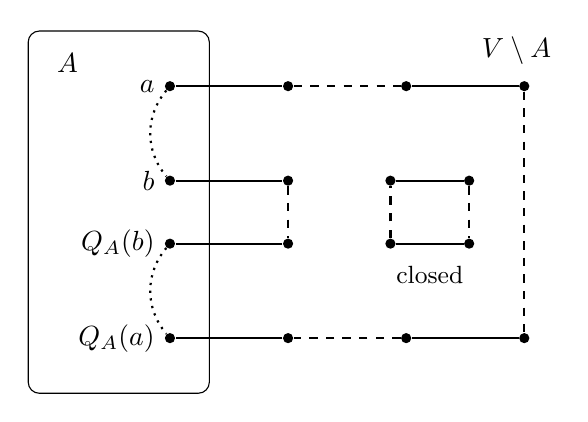
\begin{tikzpicture}[x=1cm,y=1cm,
  v/.style={circle,fill,inner sep=1.3pt},
  qe/.style={thick},
  pe/.style={thick,dashed},
  xe/.style={thick,dotted}]
\draw[rounded corners] (0,-0.3) rectangle (2.3,4.3);
\node at (0.5,3.9) {$A$};
\node at (6.2,4.05) {$V\setminus A$};
\node[v,label=left:{$a$}] (a1) at (1.8,3.6) {};
\node[v,label=left:{$b$}] (b1) at (1.8,2.4) {};
\node[v,label=left:{$Q_A(b)$}] (b2) at (1.8,1.6) {};
\node[v,label=left:{$Q_A(a)$}] (a2) at (1.8,0.4) {};
\node[v] (p1) at (3.3,3.6) {};
\node[v] (p2) at (4.8,3.6) {};
\node[v] (p3) at (6.3,3.6) {};
\node[v] (p4) at (6.3,0.4) {};
\node[v] (p5) at (4.8,0.4) {};
\node[v] (p6) at (3.3,0.4) {};
\node[v] (q1) at (3.3,2.4) {};
\node[v] (q2) at (3.3,1.6) {};
\node[v] (c1) at (4.6,2.4) {};
\node[v] (c2) at (5.6,2.4) {};
\node[v] (c3) at (5.6,1.6) {};
\node[v] (c4) at (4.6,1.6) {};
\draw[qe] (a1)--(p1);
\draw[pe] (p1)--(p2);
\draw[qe] (p2)--(p3);
\draw[pe] (p3)--(p4);
\draw[qe] (p4)--(p5);
\draw[pe] (p5)--(p6);
\draw[qe] (p6)--(a2);
\draw[qe] (b1)--(q1);
\draw[pe] (q1)--(q2);
\draw[qe] (q2)--(b2);
\draw[qe] (c1)--(c2);
\draw[pe] (c2)--(c3);
\draw[qe] (c3)--(c4);
\draw[pe] (c4)--(c1);
\node[font=\small] at (5.1,1.2) {closed};
\draw[xe] (a1) to[bend right=40] (b1);
\draw[xe] (b2) to[bend right=40] (a2);
\end{tikzpicture}
\caption{Solid edges belong to $Q$, dashed edges to $P'$ and dotted edges to a matching $X$ of $A$. The two alternating paths through $V\setminus A$ give the exit matching $Q_A=\{\{a,Q_A(a)\},\{b,Q_A(b)\}\}$, which does not depend on $X$. The $4$-cycle on the right is a closed cycle, so in this picture case (i) of Theorem~\ref{thm:contraction} applies and $H[X\cup P',Q]=0$. Without it, case (ii) gives $H[X\cup P',Q]=H_A[X,Q_A]$.}\label{fig:contraction}
\end{figure}

\begin{theorem}[Contraction]\label{thm:contraction}
Let $P,Q\in\M(V)$, let $A\subseteq V$ be nonempty and closed under $P$, and let $P'=P|_{V\setminus A}$. For every $X\in\M(A)$ the following hold.
\begin{enumerate}
\item If $Q\cup P'$ has a closed cycle, then $H[X\cup P',Q]=0$.
\item Otherwise $H[X\cup P',Q]=H_A[X,Q_A]$.
\end{enumerate}
\end{theorem}

\begin{proof}
In case (i) the vertex set of the closed cycle lies in $V\setminus A$ and is closed under $X\cup P'$ and under $Q$. It misses $A\neq\emptyset$, so $(X\cup P')\cup Q$ is disconnected. In case (ii) every vertex of $V\setminus A$ lies on one of the paths, and each path joins $a$ to $Q_A(a)$. Replacing each path by the edge $\{a,Q_A(a)\}$ turns $(X\cup P')\cup Q$ into $X\cup Q_A$ and preserves connectivity in both directions.
\end{proof}

Cygan, Kratsch and Nederlof prove their factorization of $H$~\cite[Thm.~3.4]{CKN18}, recalled in Section~\ref{subsec:complete}, with a related reduction, which removes two vertices~\cite[App.~A.1, Def.~A.1 and Lemma~A.3]{CKN18}.

% chktex-file 12
% chktex-file 36
\section{Local parity, the three-cycle relation and the Clifford action}\label{sec:threecycle}

Wales proved that, for $m\ge5$, an irreducible representation of the double cover $\St_m$ in which an element of order $3$ lying over a $3$-cycle has a quadratic minimal polynomial is a basic spin representation~\cite[Thm.~8.1]{Wales79}. This section shows that $1+\tau+\tau^2$ annihilates the row space of $H_V$ for every $3$-cycle $\tau$, and Proposition~\ref{prop:minpoly} shows that $x^2+x+1$ is then the minimal polynomial of the action of $\tau$.

Let $\F[\M(V)]$ be the $\F$-vector space with basis $e_P$, $P\in\M(V)$. For $f\in\F[\M(V)]$ write $f(Q)$ for the coefficient of $e_Q$. The \emph{fingerprint} of $P$ is the row $\varphi(P)=\sum_{Q}H[P,Q]\,e_Q$ of $H_V$, and $W(V)\subseteq\F[\M(V)]$ is the span of the fingerprints, so $W_n=W(\{0,\dots,2n-1\})$. The group $S_V$ acts on $\F[\M(V)]$ by $\rho(\sigma)e_Q=e_{\sigma Q}$. Since $H$ is invariant, $\rho(\sigma)\varphi(P)=\varphi(\sigma P)$, so $W(V)$ is a submodule, and we write $\rho_W$ for the action on it.

\subsection{Four and six points}

Lemmas~\ref{lem:four} and~\ref{lem:six} are the local parity statements of the title. They show that certain sums of three entries of $H_A$ vanish when $|A|$ is $4$ or $6$, and Theorem~\ref{thm:threecycle} reduces the general case to them.

\begin{lemma}\label{lem:four}
Let $|A|=4$. Two matchings $X,Y\in\M(A)$ satisfy $\Ham(X,Y)$ if and only if $X\ne Y$. Hence $\sum_{X\in\M(A)}H_A[X,Y]=0$ for every $Y\in\M(A)$.
\end{lemma}

\begin{proof}
Two distinct matchings of four points share no edge, and their union is a $4$-cycle. A matching shares its two edges with itself. So exactly two of the three summands are $1$.
\end{proof}

\begin{lemma}\label{lem:six}
Let $|A|=6$ and let $a,b,c,a',b',c'$ be the six points of $A$. Let $X\in\M(A)$ contain $\{a,a'\}$, $\{b,b'\}$ and $\{c,c'\}$, and let $\tau=(a\;\,b\;\,c)$. Then
\[
H_A[X,Y]+H_A[\tau X,Y]+H_A[\tau^{2}X,Y]=0\qquad\text{for every }Y\in\M(A).
\]
\end{lemma}

\begin{proof}
Put $S=\{a,b,c\}$, $T=\{a',b',c'\}$ and $X_i=\tau^{i}X$ for $i=0,1,2$. Each $X_i$ matches $S$ to $T$, and we let $x_i\colon S\to T$ be the bijection given by its edges. Since $\tau$ fixes $T$, $x_i=x_0\tau^{-i}$, so $\{x_0^{-1}x_0,x_1^{-1}x_0,x_2^{-1}x_0\}$ is the alternating group $A_3$ on $S$.

The number of edges of $Y$ between $S$ and $T$ is odd, so it is $1$ or $3$. Suppose it is $3$, so that $Y$ matches $S$ to $T$ by a bijection $y$. Following the edges of $X_i$ and $Y$ alternately shows that $X_i\cup Y$ is a $6$-cycle exactly when the permutation $x_i^{-1}y$ of $S$ is a $3$-cycle. The three permutations $x_i^{-1}y=\tau^{i}x_0^{-1}y$ form the coset of $A_3$ that contains $x_0^{-1}y$. If $x_0^{-1}y\in A_3$, they are the elements of $A_3$, and two of them are $3$-cycles. Otherwise they are the three transpositions of $S$. So the number of Hamiltonian pairs among $(X_i,Y)$ is $2$ or $0$.

Suppose instead that $Y$ has one edge $\{s,t\}$ with $s\in S$ and $t\in T$. Exactly one $i$ has $x_i(s)=t$, so exactly one $X_i$ contains $\{s,t\}$, and its union with $Y$ has a doubled edge. The other two $X_i$ share no edge with $Y$, and two edge-disjoint perfect matchings of six points form one $6$-cycle. The number of Hamiltonian pairs is $2$.
\end{proof}

\subsection{The three-cycle relation on \texorpdfstring{$W(V)$}{W(V)}}

\begin{theorem}\label{thm:threecycle}
Let $\tau\in S_V$ be a $3$-cycle and $P,Q\in\M(V)$. Then
\[
H[P,Q]+H[\tau P,Q]+H[\tau^{2}P,Q]=0.
\]
Equivalently $\varphi(P)+\varphi(\tau P)+\varphi(\tau^{2}P)=0$, and $1+\rho_W(\tau)+{\rho_W(\tau)}^2=0$ on $W(V)$.
\end{theorem}

\begin{proof}
Write $\tau=(a\;\,b\;\,c)$ and let $A$ be the union of the edges of $P$ that meet $\{a,b,c\}$. At most one edge of $P$ lies inside $\{a,b,c\}$. If one does, $|A|=4$. Otherwise the three points have distinct partners outside $\{a,b,c\}$ and $|A|=6$. The set $A$ is closed under $P$ and $\tau$ fixes $V\setminus A$ pointwise, so $\tau^{i}P=(\tau^{i}P|_A)\cup P'$ with the notation of Section~\ref{subsec:contraction}. If $Q\cup P'$ has a closed cycle, all three terms vanish by Theorem~\ref{thm:contraction}(i). Otherwise Theorem~\ref{thm:contraction}(ii) replaces each term by $H_A[\tau^{i}P|_A,Q_A]$, with the same exit matching $Q_A$ for all three. If $|A|=4$, the three matchings $\tau^{i}P|_A$ are the three matchings of $A$ and Lemma~\ref{lem:four} applies. If $|A|=6$, Lemma~\ref{lem:six} applies.
\end{proof}

\subsection{Three-cycle modules and edge relations}

The upper bound of Section~\ref{sec:basis} uses only Theorem~\ref{thm:threecycle}, so we isolate it.

\begin{definition}\label{def:tcr}
A \emph{three-cycle module} is an $\F$-vector space $M$ with a representation $\rho_M$ of $S_V$ such that $1+\rho_M(\tau)+{\rho_M(\tau)}^2=0$ for every $3$-cycle $\tau\in S_V$. For distinct $i,j\in V$ put $\Gamma_{ij}=\rho_M(\tr ij)$, and for an edge $e=\{i,j\}$ put $\Gamma_e=\Gamma_{ij}$.
\end{definition}

\begin{proposition}\label{prop:edge}
In a three-cycle module the following hold.
\begin{enumerate}
\item $\Gamma_{ij}^2=1$ for distinct $i,j$, and $\Gamma_{ij}\Gamma_{kl}=\Gamma_{kl}\Gamma_{ij}$ for distinct $i,j,k,l$.
\item $\Gamma_{ij}\Gamma_{jk}+\Gamma_{jk}\Gamma_{ij}=1$ for distinct $i,j,k$.
\item $\Gamma_{ij}+\Gamma_{jk}+\Gamma_{ik}=0$ for distinct $i,j,k$, that is, $\Gamma_{ik}=\Gamma_{ij}+\Gamma_{jk}$.
\end{enumerate}
For edges $e$ and $f$ these combine into $\Gamma_e\Gamma_f+\Gamma_f\Gamma_e=|e\cap f|\cdot 1$, with $|e\cap f|$ read modulo $2$.
\end{proposition}

\begin{proof}
Part (i) holds in every representation of $S_V$. For (ii), $\tau=\tr ij\tr jk$ is a $3$-cycle and $\tr jk\tr ij=\tau^{-1}=\tau^2$, so $\Gamma_{ij}\Gamma_{jk}+\Gamma_{jk}\Gamma_{ij}=\rho_M(\tau)+{\rho_M(\tau)}^2=1$ in characteristic $2$. For (iii), the group identity $\tr ij\tr jk\tr ij=\tr ik$ and (ii) give $\Gamma_{ik}=\Gamma_{ij}\Gamma_{jk}\Gamma_{ij}=(1+\Gamma_{jk}\Gamma_{ij})\Gamma_{ij}=\Gamma_{ij}+\Gamma_{jk}$. In the last statement $|e\cap f|=2$ gives $2\Gamma_e^2=0$, $|e\cap f|=1$ is (ii) and $|e\cap f|=0$ is (i).
\end{proof}

By Theorem~\ref{thm:threecycle}, $W(V)$ is a three-cycle module.

\subsection{The even-weight space and the Clifford homomorphism}\label{subsec:clifford}

Let $\varepsilon_v$, $v\in V$, be the standard basis of $\F^V$, let $U(V)=\{x\in\F^V:\sum_v x_v=0\}$ be the even-weight subspace, and for $i\ne j$ put $v_{ij}=\varepsilon_i+\varepsilon_j$. For an edge $e=\{i,j\}$ write $v_e=v_{ij}$. Fixing $o\in V$, every $x\in U(V)$ equals $\sum_{j\ne o}x_j v_{oj}$, so the $v_{ij}$ span $U(V)$. On $U(V)$ put
\[
\qf(x)=\tfrac12\wt(x)\bmod 2,\qquad \bq(x,y)=\sum_v x_{v}y_v=\lvert\supp x\cap\supp y\rvert\bmod2 ,
\]
where $\wt(x)=\lvert\supp x\rvert$ is the weight of $x$. Since $\wt(x+y)=\wt(x)+\wt(y)-2\lvert\supp x\cap\supp y\rvert$, we have $\qf(x+y)=\qf(x)+\qf(y)+\bq(x,y)$, so $\qf$ is a quadratic form with polar form $\bq$. The all-ones vector $\ones$ lies in $U(V)$ when $|V|$ is even, $\bq(\ones,x)=0$ for every $x\in U(V)$, and $\qf(\ones)=n\bmod 2$ when $|V|=2n$. Also $\qf(v_e)=1$ and $\bq(v_e,v_f)=|e\cap f|\bmod 2$. Let $\Cl(U(V),\qf)$ be the Clifford algebra, the quotient of the tensor algebra of $U(V)$ by the relations $x\otimes x=\qf(x)$, and $\iota\colon U(V)\to\Cl(U(V),\qf)$ the canonical map. The group $S_V$ acts on $U(V)$ by ${(\sigma x)}_k=x_{\sigma^{-1}k}$ and preserves $\qf$, so by the universal property it acts on $\Cl(U(V),\qf)$ by algebra automorphisms with $\sigma\iota(x)=\iota(\sigma x)$. For $|V|=2n$ we write $U_n=U(V)$.

\begin{theorem}\label{thm:clifford}
Let $M$ be a three-cycle module for $S_V$.
\begin{enumerate}
\item There is a unique linear map $\Gamma\colon U(V)\to\End_{\F}(M)$ with $\Gamma(v_{ij})=\Gamma_{ij}$ for all $i\ne j$.
\item $\Gamma(x)\Gamma(y)+\Gamma(y)\Gamma(x)=\bq(x,y)\cdot 1$ and ${\Gamma(x)}^2=\qf(x)\cdot 1$ for all $x,y\in U(V)$.
\item $\rho_M(\sigma)\Gamma(x){\rho_M(\sigma)}^{-1}=\Gamma(\sigma x)$ for $\sigma\in S_V$.
\item $\Gamma$ extends to an $S_V$-equivariant algebra homomorphism $\Cl(U(V),\qf)\to\End_{\F}(M)$ with $\iota(v_e)\mapsto\Gamma_e$, where $S_V$ acts on $\End_{\F}(M)$ by conjugation.
\end{enumerate}
\end{theorem}

\begin{proof}
Fix $o\in V$, put $G_j=\Gamma_{oj}$ for $j\ne o$ and $G_o=0$, and define $\Gamma(x)=\sum_j x_{j}G_j$ on $\F^V$. For $i\ne j$ both different from $o$, Proposition~\ref{prop:edge}(iii) gives $\Gamma(v_{ij})=\Gamma_{oi}+\Gamma_{oj}=\Gamma_{ij}$, and $\Gamma(v_{oj})=\Gamma_{oj}$. Uniqueness holds because the $v_{ij}$ span $U(V)$. For (ii), the anticommutator is bilinear, and on spanning vectors it equals $|e\cap f|=\bq(v_e,v_f)$ by Proposition~\ref{prop:edge}. Then ${\Gamma(x+y)}^2={\Gamma(x)}^2+{\Gamma(y)}^2+\bq(x,y)$ and $\qf(x+y)=\qf(x)+\qf(y)+\bq(x,y)$, and ${\Gamma(v_e)}^2=1=\qf(v_e)$, so induction on the number of spanning vectors in $x$ gives ${\Gamma(x)}^2=\qf(x)$. Part (iii) holds on the spanning vectors because $\sigma\tr ij\sigma^{-1}=\tr{\sigma i}{\sigma j}$ and $\sigma v_{ij}=v_{\sigma i,\sigma j}$, and both sides are linear in $x$. Part (iv) is the universal property of the Clifford algebra, and equivariance holds on the generators $\iota(x)$ by (iii).
\end{proof}

For $M=W_n$ we call the map of Theorem~\ref{thm:clifford}(iv) the \emph{Clifford action} on $W_n$.

Sections~\ref{subsec:tl} and~\ref{subsec:reduction} use the following presentation of $\Cl(U_n,\qf)$ by the elements $\iota(v_{t,t+1})$.

\begin{lemma}\label{lem:reducehom}
Let $V=\{0,\dots,2n-1\}$, let $\mathcal A$ be an $\F$-algebra and let $y_0,\dots,y_{2n-2}\in\mathcal A$ satisfy $y_t^2=1$ and $y_{s}y_t+y_{t}y_s=[|s-t|=1]$ for all $s,t$. Then there is a unique algebra homomorphism $\Cl(U_n,\qf)\to\mathcal A$ with $\iota(v_{t,t+1})\mapsto y_t$.
\end{lemma}

\begin{proof}
The $v_{t,t+1}$ form a basis of $U_n$, so there is a unique linear map $\gamma\colon U_n\to\mathcal A$ with $\gamma(v_{t,t+1})=y_t$. Its square equals $\qf$ on the basis, and its anticommutator equals $\bq$ on pairs of basis vectors, since $\bq(v_{s,s+1},v_{t,t+1})=[|s-t|=1]$ for $s\ne t$. As in the proof of Theorem~\ref{thm:clifford}(ii), ${\gamma(x)}^2=\qf(x)$ for all $x$, and the universal property applies.
\end{proof}

% chktex-file 12
% chktex-file 36
\section{The gap-swap basis, rank \texorpdfstring{$2^{n-1}$}{2\textasciicircum(n-1)} and absolute irreducibility}\label{sec:basis}

For the definitions below $V=\{0,1,\dots,2n-1\}$ with $n\ge1$. The \emph{blocks} are the pairs $\{2a,2a+1\}$ for $0\le a\le n-1$, and they form the base matching $P_0$. The \emph{gaps} are the pairs $\{2g+1,2g+2\}$ for $g\in G=\{0,\dots,n-2\}$. Put
\[
B_a=\Gamma_{2a,2a+1},\qquad \sigma_S=\prod_{g\in S}\tr{2g+1}{2g+2}\quad(S\subseteq G),\qquad X_S=\sigma_S P_0 .
\]
The gap transpositions commute, so $\sigma_S\sigma_T=\sigma_{S\triangle T}$. The matching $X_S$ is obtained from $P_0$ by exchanging the two points of each gap in $S$, and the fingerprints $\varphi(X_S)$, $S\subseteq G$, form the \emph{gap-swap basis} of $W_n$ (Theorem~\ref{thm:rank}).

\subsection{An upper bound for three-cycle modules}

\begin{proposition}\label{prop:Bw}
Let $M$ be a three-cycle module for $S_{2n}$ and let $m_0\in M$ satisfy $B_{a}m_0=m_0$ for every block $a$. Put $w_S=\rho_M(\sigma_S)m_0$. Then $\rho_M(\sigma_T)w_S=w_{T\triangle S}$ and
\[
B_{a}w_S=w_S+[a-1\in S]\,w_{S\setminus\{a-1\}}+[a\in S]\,w_{S\setminus\{a\}} .
\]
\end{proposition}

\begin{proof}
The first formula is $\sigma_T\sigma_S=\sigma_{T\triangle S}$. A block edge $\{2a,2a+1\}$ meets the gap edge of $g$ in one point exactly when $g\in\{a-1,a\}$, and is disjoint from it otherwise. By Proposition~\ref{prop:edge}, $B_a\rho_M(\sigma_{\{g\}})=\rho_M(\sigma_{\{g\}})B_a+[g\in\{a-1,a\}]$. Induction on $|S|$, starting from $B_{a}m_0=m_0$, gives the formula.
\end{proof}

\begin{theorem}\label{thm:upper}
Let $|V|=2n$ and let $M$ be a three-cycle module for $S_V$ that is spanned by the orbit of a vector $m_0$ fixed by the transpositions $\tr v{P(v)}$ of some matching $P$. Then $\dim_{\F}M\le 2^{n-1}$.
\end{theorem}

\begin{proof}
Relabel so that $V=\{0,\dots,2n-1\}$ and $P=P_0$. By Proposition~\ref{prop:Bw} the span of the $w_S$ is stable under every gap transposition and every block transposition. These are the adjacent transpositions $\tr t{t+1}$, which generate $S_{2n}$. Hence the span contains the orbit of $m_0=w_\emptyset$ and equals $M$. There are $2^{n-1}$ vectors $w_S$.
\end{proof}

\subsection{A permutation submatrix and the rank of \texorpdfstring{$H_{2n}$}{H\_2n}}

Put $w_S=\varphi(X_S)\in W_n$. This is the vector of Proposition~\ref{prop:Bw} for $M=W_n$ and $m_0=\varphi(P_0)$, since $B_a\varphi(P_0)=\varphi(\tr{2a}{2a+1}P_0)=\varphi(P_0)$. Group the points as $0\mid1,2\mid3,4\mid\dots\mid2n-3,2n-2\mid2n-1$. The matchings $X_S$ are exactly the perfect matchings that join only points of adjacent groups, which is the family of Cygan, Kratsch and Nederlof~\cite[Def.~3.1, Prop.~3.2]{CKN18}.

\begin{lemma}\label{lem:HX}
For $S,T\subseteq G$, $H[X_S,X_T]=[S\triangle T=G]$.
\end{lemma}

\begin{proof}
By invariance, $H[X_S,X_T]=H[P_0,\sigma_S\sigma_{T}P_0]=H[P_0,X_{S\triangle T}]$. Let $D\subseteq G$ with $D\ne G$ and choose a gap $g\notin D$. The set $\{0,\dots,2g+1\}$ is closed under $P_0$, and it is closed under $X_D=\sigma_{D}P_0\sigma_D$ because every gap transposition in $\sigma_D$ moves points on one side of the cut between $2g+1$ and $2g+2$. Hence $P_0\cup X_D$ is disconnected. For $D=G$ and $n\ge2$ the edges of $X_G$ are $\{0,2\}$, $\{2a-1,2a+2\}$ for $1\le a\le n-2$ and $\{2n-3,2n-1\}$, and $X_G=P_0$ when $n=1$. Contract each block to a point. The edges of $X_G$ join block $0$ to block $1$, block $a-1$ to block $a+1$, and block $n-2$ to block $n-1$, which is a connected graph on the blocks, so $P_0\cup X_G$ is connected.
\end{proof}

This is~\cite[Prop.~3.3]{CKN18} in our notation.

\begin{theorem}[Cygan, Kratsch and Nederlof]\label{thm:rank}
Let $|V|=2n\ge2$. Then $\dim_{\F}W(V)=\rank_{\F}H_V=2^{n-1}$. For $V=\{0,\dots,2n-1\}$ the vectors $w_S=\varphi(X_S)$, $S\subseteq G$, form a basis of $W_n$. The quotient $\F[\M(V)]/{\rad H_V}$ by the radical of the bilinear form with matrix $H_V$ is isomorphic to $W(V)$ as an $\F S_V$-module, through $[x]\mapsto\sum_{P}x_P\varphi(P)$.
\end{theorem}

\begin{proof}
The upper bound is Theorem~\ref{thm:upper} for $M=W(V)$, which is spanned by the orbit of one fingerprint by Proposition~\ref{prop:count}. By Lemma~\ref{lem:HX}, the submatrix of $H$ on the rows $X_S$ and the columns $X_T$ is the permutation matrix of $S\mapsto G\setminus S$, so the $\varphi(X_S)$ are linearly independent. The map $x\mapsto\sum_{P}x_P\varphi(P)$ is an equivariant surjection onto $W(V)$ whose kernel is the radical.
\end{proof}

The rank formula is~\cite[Cor.~3.5]{CKN18}. Cygan, Kratsch and Nederlof prove the upper bound by a factorization of $H$~\cite[Thm.~3.4]{CKN18}, and the proof above takes it from Theorem~\ref{thm:threecycle} alone.

\subsection{Lowering operators and the full matrix algebra}

The operator $1+B_a$ sends $w_S$ to the sum of its erasures $w_{S\setminus\{h\}}$ at the gaps $h\in S\cap\{a-1,a\}$. Summing $1+B_a$ over $a\le g$ telescopes modulo $2$ and leaves only the erasure at $g$.

\begin{proposition}\label{prop:lower}
For $g\in G$ put $\partial_g=\sum_{a\le g}(1+B_a)$ and $F_g=\Gamma_{2g+1,2g+2}$. Then
\[
\partial_{g}w_S=[g\in S]\,w_{S\setminus\{g\}},\qquad F_{g}w_S=w_{S\triangle\{g\}},\qquad \partial_g^2=0,\qquad F_g\partial_g+\partial_{g}F_g=1 .
\]
The product $\Lambda=\partial_{n-2}\cdots\partial_1\partial_0$ sends $w_G$ to $w_\emptyset$ and kills every other $w_S$.
\end{proposition}

\begin{proof}
By Proposition~\ref{prop:Bw}, $(1+B_a)w_S$ is the sum of $w_{S\setminus\{h\}}$ over $h\in S\cap\{a-1,a\}$. In $\sum_{a\le g}(1+B_a)w_S$ a term $w_{S\setminus\{h\}}$ with $h<g$ appears for $a=h$ and for $a=h+1$, and the two cancel, while the term with $h=g$ appears once. The formula for $F_g$ is Proposition~\ref{prop:Bw}, and the two relations follow on the basis. The statement on $\Lambda$ follows by applying the $\partial_g$ in increasing order of $g$.
\end{proof}

\begin{theorem}\label{thm:burnside}
Let $|V|=2n\ge2$. The algebra generated by $\rho_W(S_V)$ is $\End_{\F}W(V)$. For every field $k$ of characteristic $2$, let $\rho_k$ be the $k$-linear extension of $\rho_W$ to $k\otimes_{\F}W(V)$. Then the algebra generated by $\rho_k(S_V)$ is $\End_k(k\otimes_{\F}W(V))$, and $k\otimes_{\F}W(V)$ is irreducible.
\end{theorem}

\begin{proof}
It suffices to treat $V=\{0,\dots,2n-1\}$, since a bijection carries $W(V)$ to $W_n$ equivariantly. Let $w_S^*$ be the basis of the dual space with $w_S^*(w_T)=[S=T]$, and for $S,T\subseteq G$ let $w_S\otimes w_T^*$ be the matrix unit $u\mapsto w_T^*(u)\,w_S$. The algebra $\mathcal A$ generated by the $\partial_g$ and the $F_g$ lies in the algebra generated by $\rho_W(S_{2n})$, and it contains the rank-one map $\Lambda=w_\emptyset\otimes w_G^*$ of Proposition~\ref{prop:lower}. The elements $\rho_W(\sigma_S)\in\mathcal A$ carry $w_\emptyset$ to $w_S$, and $w_G^*\circ\rho_W(\sigma_{T\triangle G})=w_T^*$. So $\mathcal A$ contains every matrix unit $w_S\otimes w_T^*$, and $\mathcal A=\End_{\F}W_n$. The same matrix units span $\End_k(k\otimes_{\F}W_n)$ over $k$, and a subspace stable under the full matrix algebra is $0$ or everything.
\end{proof}

\subsection{Corollaries and Maas's matrices}

\begin{corollary}\label{cor:clsurj}
For $n\ge1$ the Clifford action $\Cl(U_n,\qf)\to\End_{\F}W_n$ of Theorem~\ref{thm:clifford} is surjective.
\end{corollary}

\begin{proof}
Its image contains $\Gamma_{ij}=\rho_W(\tr ij)$ for all $i\ne j$, and transpositions generate $S_{2n}$. Apply Theorem~\ref{thm:burnside}.
\end{proof}

The vector $\ones$ spans the radical of $\bq$ on $U_n$, and the next proposition says how it acts.

\begin{proposition}\label{prop:matchingsum}
Let $n\ge1$ and let $P$ be any perfect matching of $\{0,\dots,2n-1\}$. Then $\sum_{e\in P}\Gamma_e=\Gamma(\ones)=(n\bmod 2)\cdot1$ on $W_n$.
\end{proposition}

\begin{proof}
The vector $\ones$ is $\sum_{e\in P}v_e$ for every $P$. Each $\Gamma_e$ with $e\in P_0$ fixes $\varphi(P_0)$, so $\Gamma(\ones)\varphi(P_0)=n\,\varphi(P_0)$. By Theorem~\ref{thm:clifford}(iii), $\Gamma(\ones)$ commutes with every $\rho_W(\sigma)$, because $\sigma\ones=\ones$. The fingerprints $\varphi(\sigma P_0)=\rho_W(\sigma)\varphi(P_0)$ span $W_n$, so $\Gamma(\ones)=n$ on $W_n$.
\end{proof}

The next proposition shows that $W_n$ satisfies the condition on the minimal polynomial in Wales's theorem (Section~\ref{subsec:prior}).

\begin{proposition}\label{prop:minpoly}
Let $n\ge2$, let $k$ be a field of characteristic $2$ and let $\tau$ be a $3$-cycle. The minimal polynomial of $\rho_k(\tau)$ on $k\otimes_{\F}W_n$ is $x^2+x+1$.
\end{proposition}

\begin{proof}
By Theorem~\ref{thm:threecycle} the minimal polynomial divides $x^2+x+1$. Suppose $\rho_k(\tau)=c\cdot1$. Since $\tau$ is conjugate to $\tau^{-1}$, $c=c^{-1}$, so $c=1$ in characteristic $2$, and then $1+c+c^2=1\ne0$. So $\rho_k(\tau)$ is not a scalar.
\end{proof}

\begin{proposition}\label{prop:maas}
Let $n\ge1$ and index the basis $w_S$ of $W_n$ by the subsets $S\subseteq G$, read as bit vectors of length $n-1$. In this basis the gap transposition $\tr{2g+1}{2g+2}$ flips bit $g$, and the block transposition $\tr{2a}{2a+1}$ acts by $1+\partial_{a-1}+\partial_a$, where $\partial_{-1}=\partial_{n-1}=0$. These are the matrices $T_{t+1}$, $0\le t\le2n-2$, of Maas's construction over $\F$~\cite[Table~1]{Maas10}, read in characteristic $2$ and with the bits ordered so that each doubling step adds the last bit. For $2n\ge4$ Maas shows that they give a basic spin representation of $\St_{2n}$ over $\F$~\cite[Cor.~13]{Maas10}.
\end{proposition}

\begin{proof}
The action on the basis is Propositions~\ref{prop:Bw} and~\ref{prop:lower}. Over $\F$ Maas starts from the matrix $T_1=(1)$ of $\St_2$ and alternates two steps~\cite[Table~1]{Maas10}. Write $T_1,\dots,T_{m-1}$ for the matrices of $\St_m$. In characteristic $2$ the steps are as follows.
\begin{itemize}
\item From even $m$ to $m+1$, the doubling step of~\cite[Lemma~5]{Maas10} replaces $T_{m-1}$, and each $T_i$ with $i\le m-2$, by
\[
\begin{pmatrix}T_{m-1}&1\\0&T_{m-1}\end{pmatrix}\qquad\text{and}\qquad\begin{pmatrix}T_i&0\\0&T_i\end{pmatrix},
\]
and adds $T_m=\bigl(\begin{smallmatrix}0&1\\1&0\end{smallmatrix}\bigr)$.
\item From odd $m$ to $m+1$, the step of~\cite[Lemma~7]{Maas10} with $p=2$ adds $T_m=J$ when $m+1\equiv0\pmod4$ and $T_m=J+1$ when $m+1\equiv2\pmod4$, where $J=\sum_{j\le m-1}jT_j$, which modulo $2$ is the sum of the $T_j$ with $j$ odd.
\end{itemize}
We show by induction on $n$ that for $\St_{2n}$ the matrix $T_{t+1}$ is the matrix of $\tr t{t+1}$ in the statement. For $n=1$, $T_1=(1)$ is the action of $\tr01$ on the one-dimensional space $W_1$. Suppose the claim holds for $\St_{2n-2}$, on bit vectors of length $n-2$. The doubling step adds bit $n-2$, and in its block form the first block is the bit vectors with this bit clear. A block diagonal matrix with two diagonal blocks $T$ is $T$ acting on the other bits, so the flips of bits $g\le n-3$ and the matrices $1+\partial_{a-1}+\partial_a$ with $a\le n-3$ stay as in the statement. The matrix $T_{2n-3}$ of $\tr{2n-4}{2n-3}$ was $1+\partial_{n-3}$, and
\[
\begin{pmatrix}1+\partial_{n-3}&1\\0&1+\partial_{n-3}\end{pmatrix}=1+\partial_{n-3}+\partial_{n-2},
\]
because $\partial_{n-2}$ clears bit $n-2$. The new matrix $T_{2n-2}$ flips bit $n-2$, which is the action of $\tr{2n-3}{2n-2}$. The step of~\cite[Lemma~7]{Maas10} then adds $T_{2n-1}$. Here
\[
J=\sum_{a=0}^{n-2}T_{2a+1}=\sum_{a=0}^{n-2}(1+\partial_{a-1}+\partial_a)=(n-1)\cdot1+\partial_{n-2},
\]
since each $\partial_g$ with $g\le n-3$ occurs for $a=g$ and for $a=g+1$. The extra $1$ is added exactly when $2n\equiv2\pmod4$, that is, when $n$ is odd. In both cases $T_{2n-1}=1+\partial_{n-2}$, the action of $\tr{2n-2}{2n-1}$.
\end{proof}

\begin{remark}\label{rem:maas}
The coordinate map of the basis $w_S$ is therefore an explicit isomorphism from $W_n$ to Maas's model that carries $\tr t{t+1}$ to $T_{t+1}$. Maas calls his model a basic spin representation on the authority of Wales's theorem~\cite[Thm.~1]{Maas10}. Section~\ref{sec:spin} identifies $W_n$ with $D^{(n+1,n-1)}$ and with the reductions of the Clifford spin modules without that input.
\end{remark}

% chktex-file 12
% chktex-file 36
\section{Presentations by three-cycles, Brauer operations and Temperley--Lieb}\label{sec:presentations} % chktex 8

This section shows that the three-cycle relations are the only linear relations among fingerprints (Theorem~\ref{thm:presentation}). It then shows that the Brauer cup and cap maps descend to the quotients by these relations (Proposition~\ref{prop:cupcap}), and it presents $W_n$ as a quotient of a module over the Temperley--Lieb algebra at loop value $0$ (Theorem~\ref{thm:delta}). % chktex 8

We write $\Theta\colon\F[\M(V)]\to W(V)$ for the equivariant surjection $e_P\mapsto\varphi(P)$. Let $R_3\subseteq\F[\M(V)]$ be the span of the \emph{three-cycle orbit sums} $e_P+e_{\tau P}+e_{\tau^{2}P}$ over all $P$ and all $3$-cycles~$\tau$.

\subsection{Completeness of the three-cycle relations}\label{subsec:complete}

\begin{theorem}\label{thm:presentation}
Let $|V|=2n\ge2$ and $\Wt(V)=\F[\M(V)]/R_3$. Then $\Theta$ induces an isomorphism of $\F S_V$-modules $\Wt(V)\cong W(V)$, and
\[
\ker\Theta=\rad H_V=R_3 .
\]
For $V=\{0,\dots,2n-1\}$ and every $P\in\M_n$,
\[
e_P\equiv\sum_{S\subseteq G}H[P,X_{G\setminus S}]\,e_{X_S}\pmod{R_3}.
\]
\end{theorem}

\begin{proof}
By Theorem~\ref{thm:threecycle}, $R_3\subseteq\ker\Theta$, and $\ker\Theta=\rad H_V$ by Theorem~\ref{thm:rank}. By definition of $R_3$, $\Wt(V)$ is a three-cycle module, and it is spanned by the orbit of the class of $e_{P}$ for any $P$, which is fixed by the transpositions $\tr v{P(v)}$. Theorem~\ref{thm:upper} gives $\dim\Wt(V)\le2^{n-1}=\dim W(V)$, so the surjection $\Wt(V)\to W(V)$ is an isomorphism. For the normal form, write $\varphi(P)=\sum_{S}c_S\varphi(X_S)$ and compare the coefficients of $e_{X_{G\setminus T}}$. By Lemma~\ref{lem:HX} the coefficient of $e_{X_{G\setminus T}}$ in $\varphi(X_S)$ is $[S=T]$, so $c_T=H[P,X_{G\setminus T}]$. Hence $e_P-\sum_{S}c_{S}e_{X_S}$ lies in $\ker\Theta=R_3$.
\end{proof}

The normal form is the factorization $H[P,Q]=\sum_S H[P,X_{G\setminus S}]H[X_S,Q]$ of Cygan, Kratsch and Nederlof~\cite[Thm.~3.4]{CKN18}, read as a rewriting rule modulo the three-cycle relations.

\subsection{The Brauer pairing, cups and caps}\label{subsec:brauer}

The matrix $H$ is one coefficient of the following pairing, which counts the loops formed by two matchings. We call it the Brauer loop pairing, and the maps $\cupop_{ab}$ and $\capop_{ab}$ below Brauer cups and caps, after Brauer~\cite{Brauer37}. Over the polynomial ring $\F[\delta]$ put
\[
\pr{x,y}_\delta=\sum_{P,Q\in\M(V)}x_{P}y_Q\,\delta^{\kappa(P\cup Q)}\qquad(x,y\in\F[\M(V)]).
\]

\begin{proposition}\label{prop:brauer}
The coefficient of $\delta^1$ in $\pr{x,y}_\delta$ is $x^{\mathsf T}H_{V}y$.
\end{proposition}

\begin{proof}
On basis vectors this is $H[P,Q]=[\kappa(P\cup Q)=1]$.
\end{proof}

For distinct $a,b\in V$ let $\cupop_{ab}\colon\F[\M(V\setminus\{a,b\})]\to\F[\M(V)]$ send $e_Q$ to $e_{Q\cup\{ab\}}$, and let $\capop_{ab}\colon\F[\M(V)]\to\F[\M(V\setminus\{a,b\})]$ send $e_F$ to $[ab\notin F]\,e_{F/ab}$, with the matching $F/ab$ of Section~\ref{subsec:setup}. Let $R_4\subseteq\F[\M(V)]$ be the span of the \emph{four-switch sums} $e_{E\cup\{ab,cd\}}+e_{E\cup\{ac,bd\}}+e_{E\cup\{ad,bc\}}$, where $a,b,c,d$ are distinct and $E$ is a perfect matching of $V\setminus\{a,b,c,d\}$.

Part (ii) of the next proposition is the input to Lemma~\ref{lem:sym3}, which makes the action of Theorem~\ref{thm:delta} well defined.

\begin{proposition}\label{prop:cupcap}
Let $a\ne b$ and $|V|\ge4$.
\begin{enumerate}
\item $H[Q\cup\{ab\},F]=[ab\notin F]\,H[Q,F/ab]$ for $Q\in\M(V\setminus\{a,b\})$ and $F\in\M(V)$. Hence $\cupop_{ab}$ and $\capop_{ab}$ are adjoint for the forms with matrices $H$.
\item $R_4\subseteq R_3$, and $\cupop_{ab}(\capop_{ab}x)+x+\tr abx\in R_4$ for every $x\in\F[\M(V)]$.
\item $\cupop_{ab}$ maps $R_3(V\setminus\{a,b\})$ into $R_3(V)$, bijections $V\to V'$ map $R_3(V)$ into $R_3(V')$, and $\capop_{ab}$ maps $R_3(V)$ into $R_3(V\setminus\{a,b\})$. So cups, caps and bijections descend to the quotients $\Wt$, and on $\Wt(V)$ the composite $\cupop_{ab}\capop_{ab}$ acts as $1+\tr ab$.
\end{enumerate}
\end{proposition}

\begin{proof}
(i) Apply Theorem~\ref{thm:contraction} with $A=V\setminus\{a,b\}$, which is nonempty because $|V|\ge4$, and the matching $Q\cup\{ab\}$, whose part off $A$ is the edge $ab$. If $ab\in F$, then $\{a,b\}$ is closed under both matchings and $H=0$. Otherwise the exit matching of $F$ on $A$ is $F/ab$, since the alternating path through $\{a,b\}$ is $F(a),a,b,F(b)$.

(ii) A four-switch sum on $\{a,X(a),c,X(c)\}$ is the orbit sum of $X$ under the $3$-cycle $\tr a{X(a)}\tr ac$, so $R_4\subseteq R_3$. If $ab\in F$, then $\tr abF=F$ and $\capop_{ab}e_F=0$, so the element is $2e_F=0$. If $ab\notin F$, then $(F/ab)\cup\{ab\}=\tr{F(a)}bF$, and $e_F+e_{\tr{F(a)}bF}+e_{\tr abF}$ is the four-switch sum of the three matchings that agree with $F$ off $\{a,b,F(a),F(b)\}$.

(iii) A $3$-cycle of $V\setminus\{a,b\}$ is a $3$-cycle of $V$ that fixes $a$ and $b$, and bijections carry $3$-cycles to $3$-cycles. For caps, $R_3=\rad H$ on both vertex sets by Theorem~\ref{thm:presentation}, and $\capop_{ab}$ maps $\rad H_V$ into $\rad H_{V\setminus\{a,b\}}$ by the adjunction (i), which needs $|V\setminus\{a,b\}|\ge2$. The last statement is (ii).
\end{proof}

\begin{remark}\label{rem:boundary}
At $|V|=2$ part (i) fails, since $H[\{ab\},\{ab\}]=1$ while $\capop_{ab}e_{\{ab\}}=0$. This is why caps descend only for $n\ge2$.
\end{remark}

\subsection{Temperley--Lieb at \texorpdfstring{$\delta=0$}{delta=0} and the Jones--Wenzl quotient}\label{subsec:tl} % chktex 8

Over $\F$ at loop value $0$ the elements $s_i=1+e_i$ of the Temperley--Lieb algebra satisfy the Coxeter relations of the symmetric group (Lemma~\ref{lem:conj}), and the Jones--Wenzl idempotent $f_3$ on three strands is $1+\tau+\tau^2$ for the $3$-cycle $\tau=s_{0}s_1$ (Proposition~\ref{prop:jw}). So the quotient by $f_3$ imposes the relation of Theorem~\ref{thm:threecycle}, and this subsection identifies the quotient with $\Cl(U_n,\qf)$. % chktex 8

Let $\mathcal O$ be a commutative ring and $\delta\in\mathcal O$. The Temperley--Lieb algebra $\TL_N(\delta)$~\cite{Jones83,TL71} is generated by $e_0,\dots,e_{N-2}$ with $e_i^2=\delta e_i$, $e_{i}e_{j}e_i=e_i$ for $|i-j|=1$ and $e_{i}e_j=e_{j}e_i$ for $|i-j|\ge2$. We think of $e_i$ as acting on the strands $i$ and $i+1$ of $N$ strands numbered $0,\dots,N-1$. When $\delta^2-1$ is a unit, put % chktex 8
\[
f_3=1-\frac{\delta}{\delta^2-1}(e_0+e_1)+\frac{1}{\delta^2-1}(e_{0}e_1+e_{1}e_0)\in\TL_3(\delta),
\]
the Jones--Wenzl idempotent on three strands~\cite{Wenzl87}. % chktex 8

\begin{proposition}\label{prop:jw}
Let $\delta^2-1$ be a unit in $\mathcal O$.
\begin{enumerate}
\item $e_{i}f_3=f_{3}e_i=0$ for $i=0,1$, and $f_3^2=f_3$.
\item If $\delta=-2$ and $3$ is a unit, then with $s_i=1+e_i$,
\[
1+s_{0}s_1+s_{1}s_0=3f_3 .
\]
\item Over $\F$ at $\delta=0$, $f_3=1+e_{0}e_1+e_{1}e_0=1+s_{0}s_1+s_{1}s_0$.
\end{enumerate}
\end{proposition}

\begin{proof}
(i) The coefficient of $e_0$ in $e_{0}f_3$ is $1-\delta^2/(\delta^2-1)+1/(\delta^2-1)=0$ after using $e_0^2=\delta e_0$ and $e_{0}e_{1}e_0=e_0$, and the coefficient of $e_{0}e_1$ is $-\delta/(\delta^2-1)+\delta/(\delta^2-1)=0$. The other identities are symmetric, and $f_3^2=f_3$ follows because $f_3-1$ is a combination of words that end in $e_0$ or $e_1$, so $(f_3-1)f_3=0$. Parts (ii) and (iii) are direct expansions, with $\delta^2-1=3$ in (ii) and $\delta^2-1=1$ in (iii).
\end{proof}

For $N\ge3$ and $0\le k\le N-3$ let $f_3^{(k)}=1+e_{k}e_{k+1}+e_{k+1}e_k\in\TL_N(0)$ be the copy of $f_3$ over $\F$ at $\delta=0$ on the strands $k$, $k+1$, $k+2$. Let $\pr{f_3}$ be the two-sided ideal of $\TL_{2n}(0)$ generated by all $f_3^{(k)}$. It is $0$ when $n=1$.

\begin{lemma}\label{lem:conj}
In $\TL_N(0)$ over $\F$ put $s_i=1+e_i$. Then $s_i^2=1$, $s_{k}e_{i}s_k=e_i$ for $|i-k|\ge2$, and $s_{i}s_{j}e_{i}s_{j}s_i=e_j$ for $|i-j|=1$. Hence ${(s_{i}s_j)}^3=1$ for $|i-j|=1$. For $0\le k\le N-4$ and $\omega_k=s_{k}s_{k+1}s_{k+2}$,
\[
f_3^{(k+1)}=\omega_{k}f_3^{(k)}\omega_k^{-1}.
\]
In particular, for $n\ge2$ the ideal $\pr{f_3}$ of $\TL_{2n}(0)$ is generated by $f_3=f_3^{(0)}$.
\end{lemma}

\begin{proof}
In characteristic $2$, $s_i^2=1+2e_i+e_i^2=1$. If $z^2=0$ and $zx=xz$, then $(1+z)x(1+z)=x+2xz+z^{2}x=x$, which gives $s_{k}e_{i}s_k=e_i$ for $|i-k|\ge2$. Let $|i-j|=1$ and write $x=e_i$ and $y=e_j$, so $x^2=0$, $xyx=x$ and $yxy=y$. Then $(1+y)x(1+y)=x+y+xy+yx$, and multiplying on the left by $1+x$ gives $y+yx$, using $x^2=0$ and $xyx=x$. Multiplying on the right by $1+x$ gives $y+yx+yx+yx^2=y$. This proves $s_{i}s_{j}e_{i}s_{j}s_i=e_j$. Expanding $e_i=s_i+1$ in this identity gives $s_{i}s_{j}s_{i}s_{j}s_i=s_j$, hence ${(s_{i}s_j)}^3=1$. Now $\omega_k^{-1}=s_{k+2}s_{k+1}s_k$, and the two identities give $\omega_{k}e_k\omega_k^{-1}=s_{k}s_{k+1}e_{k}s_{k+1}s_k=e_{k+1}$ and $\omega_{k}e_{k+1}\omega_k^{-1}=s_k(s_{k+1}s_{k+2}e_{k+1}s_{k+2}s_{k+1})s_k=s_{k}e_{k+2}s_k=e_{k+2}$. Conjugation is an algebra automorphism, so it carries $f_3^{(k)}=1+e_{k}e_{k+1}+e_{k+1}e_k$ to $f_3^{(k+1)}$.
\end{proof}

\begin{theorem}\label{thm:tlcl}
For $n\ge1$ there is an isomorphism of $\F$-algebras
\[
\TL_{2n}(0)/\pr{f_3}\xrightarrow{\ \sim\ }\Cl(U_n,\qf),\qquad e_i\mapsto1+\iota(v_{i,i+1})\quad(0\le i\le2n-2),
\]
whose inverse sends $\iota(v_{i,i+1})$ to $1+e_i$.
\end{theorem}

\begin{proof}
Put $a_i=1+\iota(v_{i,i+1})$. Then $a_i^2=1+\qf(v_{i,i+1})=0$. For adjacent $i,j$ write $x=\iota(v_{i,i+1})$ and $y=\iota(v_{j,j+1})$, so $x^2=y^2=1$ and $xy+yx=\bq(v_{i,i+1},v_{j,j+1})=1$. Expanding with $x^2=1$ gives $(1+x)(1+y)(1+x)=y+(xy+yx)+xyx=y+1+xyx$, and $xyx=x(1+xy)=x+y$, so $a_{i}a_{j}a_i=1+x=a_i$. Far generators commute because their vectors are orthogonal. Hence $e_i\mapsto a_i$ defines an algebra map from $\TL_{2n}(0)$. It kills every $f_3^{(i)}=1+e_{i}e_{i+1}+e_{i+1}e_i$, because $1+(1+x)(1+y)+(1+y)(1+x)=1+xy+yx=0$ for $x=\iota(v_{i,i+1})$ and $y=\iota(v_{i+1,i+2})$. In the other direction, in $\TL_{2n}(0)/\pr{f_3}$ the elements $s_i=1+e_i$ satisfy $s_i^2=1$ and $s_{i}s_j=s_{j}s_i$ for $|i-j|\ge2$, and for $0\le i\le2n-3$
\[
s_{i}s_{i+1}+s_{i+1}s_i=e_{i}e_{i+1}+e_{i+1}e_i=1+f_3^{(i)}=1 .
\]
These are the Clifford relations on the basis $v_{0,1},\dots,v_{2n-2,2n-1}$ of $U_n$, on which $\qf$ is $1$ and whose Gram matrix for $\bq$ is the adjacency matrix of a path. By Lemma~\ref{lem:reducehom}, $\iota(v_{i,i+1})\mapsto s_i$ defines an algebra map from $\Cl(U_n,\qf)$. The two maps are inverse on generators.
\end{proof}

\subsection{The four-switch quotient}

Let $\Delta(V)=\F[\M(V)]/R_4$ and $\Delta_{2n}(0)=\Delta(\{0,\dots,2n-1\})$. Since $R_4$ is $S_V$-stable, $S_V$ acts on $\Delta(V)$.

\begin{lemma}\label{lem:sym3}
For distinct $a,b,c\in V$ and every $x\in\F[\M(V)]$, $\sum_{\sigma\in S_{\{a,b,c\}}}\sigma x\in R_4$.
\end{lemma}

\begin{proof}
Write $t=\tr ab$, $u=\tr bc$ and $\Pi=\cupop_{ab}\capop_{ab}$. Since $S_{\{a,b,c\}}=\{1,u,tu\}\cdot\{1,t\}$, the sum is $(1+t)x+(1+t)u(1+t)x$. By Proposition~\ref{prop:cupcap}(ii), $(1+t)x\equiv\Pi x$ modulo $R_4$, for every $x$. The cap of the swapped cup is the identity, $\capop_{ab}\circ u\circ\cupop_{ab}=1$, since $u(Q\cup\{ab\})$ contains $ac$ and $(u(Q\cup\{ab\}))/ab=Q$. With $y=u\Pi x$ we get $(1+t)y\equiv\Pi y=\cupop_{ab}(\capop_{ab}u\cupop_{ab})\capop_{ab}x=\Pi x$. Since $R_4$ is stable under $S_V$, $(1+t)u(1+t)x\equiv(1+t)u\Pi x=(1+t)y$, and the sum is congruent to $\Pi x+\Pi x=0$.
\end{proof}

\begin{theorem}\label{thm:delta}
Let $n\ge2$.
\begin{enumerate}
\item The rule $e_i\mapsto1+\tr i{i+1}$, $0\le i\le2n-2$, defines an action of $\TL_{2n}(0)$ on $\Delta_{2n}(0)$, under which $f_3$ acts as $1+\tau_0+\tau_0^2$ for the $3$-cycle $\tau_0=\tr01\tr12$.
\item $\pr{f_3}\Delta_{2n}(0)=R_3/R_4$.
\item $\Theta$ induces an $S_{2n}$-isomorphism $\Delta_{2n}(0)/\pr{f_3}\Delta_{2n}(0)\cong W_n$ with $[e_P]\mapsto\varphi(P)$, and $\pr{f_3}\Delta_{2n}(0)$ is the radical of the form induced by $H$ on $\Delta_{2n}(0)$.
\end{enumerate}
\end{theorem}

\begin{proof}
(i) Write $x=\tr i{i+1}$ and $y=\tr{i+1}{i+2}$. Then ${(1+x)}^2=0$, and $(1+x)(1+y)(1+x)=1+x$ is equivalent to $\sum_{\sigma\in S_{\{i,i+1,i+2\}}}\sigma=0$, which holds on $\Delta_{2n}(0)$ by Lemma~\ref{lem:sym3}. The expression for $f_3$ is Proposition~\ref{prop:jw}(iii). (ii) Each $f_3^{(k)}$ acts as $1+\tau_k+\tau_k^2$ for a $3$-cycle $\tau_k$, so $\pr{f_3}\Delta_{2n}(0)\subseteq R_3/R_4$. Conversely every $3$-cycle is conjugate to $\tau_0$, and $\pr{f_3}\Delta_{2n}(0)$ is stable under $S_{2n}$, since $S_{2n}$ is generated by the transpositions $\tr i{i+1}$, through which the elements $s_i=1+e_i$ act. So for $\tau=\sigma\tau_0\sigma^{-1}$ and every $P$, $(1+\tau+\tau^2)[e_P]=\sigma(1+\tau_0+\tau_0^2)\sigma^{-1}[e_P]$ lies in $\pr{f_3}\Delta_{2n}(0)$, and these elements span $R_3/R_4$. (iii) follows from (ii), $R_4\subseteq R_3$ and Theorem~\ref{thm:presentation}.
\end{proof}

Section~\ref{subsec:specht} identifies $\Delta_{2n}(0)$ with the Specht module $S^{(n,n)}$ over $\F$, and Theorem~\ref{thm:step1}(iii) shows that on its basis of noncrossing matchings $e_i$ acts by the rule that defines the standard module of $\TL_{2n}(0)$ with no through strands (see the paragraph after Theorem~\ref{thm:step1}). With Theorems~\ref{thm:tlcl} and~\ref{thm:delta}, $W_n$ is the quotient of this standard module by the Jones--Wenzl ideal, and the algebra acting on it is $\TL_{2n}(0)/\pr{f_3}\cong\Cl(U_n,\qf)$. % chktex 8

% chktex-file 12
% chktex-file 36
\section{Identification with the \texorpdfstring{$2$}{2}-modular basic spin representation}\label{sec:spin}

This section identifies $W_n$ in two ways. Section~\ref{subsec:specht} proves the identification in the title, $W_n\cong D^{(n+1,n-1)}$, from James's definitions of Specht modules, and it needs no Clifford algebra in characteristic $0$. Sections~\ref{subsec:cover} to~\ref{subsec:reduction} work with the Clifford algebra over an algebraically closed field of characteristic $0$ through which the double cover $\St_{2n}$ acts, and prove that the reduction modulo $2$ of each of its finite-dimensional simple modules is $k\otimes_{\F}W_n$, for every lattice and every reduction map.

\subsection{The double cover and the root form}\label{subsec:cover}

For $m\ge2$ let $\St_m$ be the group generated by $z,t_0,\dots,t_{m-2}$ with the relations
\[
z^2=1,\quad z\text{ central},\quad t_j^2=z,\quad {(t_{j}t_{j+1})}^3=z,\quad {(t_{i}t_j)}^2=z\ (j\ge i+2).
\]
The map $t_j\mapsto\tr j{j+1}$, $z\mapsto1$ is a surjection $\pi\colon\St_m\to S_m$. This is the presentation used by Maas~\cite{Maas10}, with his generators $t_1,\dots,t_{m-1}$ numbered from $0$. The ordinary basic spin representations were constructed by Schur~\cite{Schur11}, as Maas recalls in his introduction~\cite{Maas10}.

Let $\mathcal O$ be a commutative ring. On $\mathcal O^{m-1}$ with standard basis $b_0,\dots,b_{m-2}$ put
\[
Q_{\mathrm S}(x)=-\sum_{j=0}^{m-2}x_j^2+\sum_{j=0}^{m-3}x_{j}x_{j+1},
\]
the negative of the root form of type $A_{m-1}$. Then $Q_{\mathrm S}(b_j)=-1$, and the polar form $Q_{\mathrm S}(x+y)-Q_{\mathrm S}(x)-Q_{\mathrm S}(y)$ takes the values $-2$ on the diagonal, $1$ on adjacent basis vectors and $0$ otherwise. In the Clifford algebra $\Cl_{\mathcal O}(Q_{\mathrm S})$ the elements $T_j=\iota(b_j)$ satisfy $T_j^2=-1$, $T_{j}T_{j+1}+T_{j+1}T_j=1$ and $T_{i}T_j+T_{j}T_i=0$ for $|i-j|\ge2$.

\begin{lemma}\label{lem:schurhom}
Let $\mathcal A$ be a ring and $T_0,\dots,T_{m-2}\in\mathcal A$ with $T_j^2=-1$, adjacent anticommutators $1$ and distant anticommutators $0$. Then $t_j\mapsto T_j$, $z\mapsto-1$ defines a homomorphism $\St_m\to\mathcal A^\times$.
\end{lemma}

\begin{proof}
The element $-1$ is central with square $1$, and $T_j^2=-1$. Let $a^2=b^2=-1$ and $c=ab$. If $ab+ba=1$, then $c^2=a(ba)b=a(1-ab)b=c-a^{2}b^2=c-1$, so $c^3=c^2-c=-1$. If $ab+ba=0$, then $c^2=-a^{2}b^2=-1$. So the images satisfy the defining relations.
\end{proof}

Taking $T_j=\iota(b_j)$ in $\Cl_{\mathcal O}(Q_{\mathrm S})$ gives a homomorphism $\St_m\to{\Cl_{\mathcal O}(Q_{\mathrm S})}^\times$, which we call the \emph{Clifford homomorphism}. In characteristic $2$, for $m=2n$, Lemma~\ref{lem:schurhom} applies to the elements $\iota(v_{j,j+1})$, $0\le j\le2n-2$, of $\Cl(U_n,\qf)$, since ${\iota(v_{j,j+1})}^2=\qf(v_{j,j+1})=1=-1$ and the anticommutator of $\iota(v_{i,i+1})$ and $\iota(v_{j,j+1})$ is $\bq(v_{i,i+1},v_{j,j+1})$, which is $1$ for $|i-j|=1$ and $0$ for $|i-j|\ge2$. It gives a homomorphism $\St_{2n}\to{\Cl(U_n,\qf)}^\times$ with $t_j\mapsto\iota(v_{j,j+1})$ and $z\mapsto1$, and composed with the Clifford action on $W_n$ it equals $\rho_W\circ\pi$, because $\iota(v_{j,j+1})$ acts as $\Gamma_{j,j+1}=\rho_W(\tr j{j+1})$.

\subsection{An upper bound in characteristic \texorpdfstring{$0$}{0} and a lower bound in characteristic \texorpdfstring{$2$}{2}}\label{subsec:bounds}

Proposition~\ref{prop:jsystem} and Theorem~\ref{thm:char0} bound the dimension of a Clifford spin module from above. Theorem~\ref{thm:vacuum} shows that every nonzero $\Cl(U_n,\qf)$-module in characteristic~$2$ contains a copy of $k\otimes_{\F}W_n$.

\begin{proposition}\label{prop:jsystem}
Let $K$ be a field with $2\ne0$ that contains an element $I$ with $I^2=-1$. Let $Y\ne0$ be a finite-dimensional $K$-vector space and $J_0,\dots,J_{2p}$ pairwise anticommuting operators on $Y$ with $J_r^2=1$. If the only subspaces of $Y$ stable under every $J_r$ are $0$ and $Y$, then $\dim_{K}Y\le2^p$.
\end{proposition}

\begin{proof}
For $i<p$ put $J_i^+=J_{2i}+IJ_{2i+1}$ and $J_i^-=J_{2i}-IJ_{2i+1}$. Then
\[
{(J_i^+)}^2={(J_i^-)}^2=0,\qquad J_i^+J_i^-+J_i^-J_i^+=4,
\]
and for $i\ne j$ the operators $J_i^\pm$ anticommute with $J_j^\pm$ and with $J_{2p}$.

Each $J_i^+$ anticommutes with the others, so it preserves their joint kernel. Since ${(J_i^+)}^2=0$, it has a nonzero kernel on every nonzero subspace that it preserves. Induction on $i$ gives a nonzero joint kernel of $J_0^+,\dots,J_{p-1}^+$. The operator $J_{2p}$ preserves this joint kernel and $J_{2p}^2=1$, so the joint kernel contains a vector $y_0\ne0$ with $J_{2p}y_0=\pm y_0$.

Let $A_0=Ky_0$ and $A_{j+1}=A_j+J_j^-A_j$. Then $A_p$ is spanned by the $2^p$ vectors $J_{i_1}^-\cdots J_{i_r}^-y_0$ with $i_1<\cdots<i_r$, so $\dim A_p\le2^p$.

Moving $J_i^+$, $J_i^-$ or $J_{2p}$ to the right through such a product, using the anticommutation relations, ${(J_i^-)}^2=0$, $J_i^+J_i^-=4-J_i^-J_i^+$, $J_i^+y_0=0$ and $J_{2p}y_0=\pm y_0$, shows that $A_p$ is stable under all of them. Since $J_{2i}=(J_i^++J_i^-)/2$ and $J_{2i+1}=(J_i^+-J_i^-)/(2I)$, $A_p$ is stable under every $J_r$, so $A_p=Y$.
\end{proof}

\begin{definition}\label{def:basicspin}
Let $K$ be an algebraically closed field of characteristic $0$ and $n\ge1$. A \emph{Clifford spin module} of $\St_{2n}$ over $K$ is a finite-dimensional simple module $Y$ over $\Cl_K(Q_{\mathrm S})$, with $Q_{\mathrm S}$ on $K^{2n-1}$, regarded as a representation of $\St_{2n}$ through the Clifford homomorphism.
\end{definition}

\todo[inline]{Source needed. A read reference, with locator, stating that the Clifford spin modules of Definition~\ref{def:basicspin} are the two associate basic spin representations of $\St_{2n}$ of Schur, as used by Maas~\cite[Thm.~1]{Maas10}. Candidates are Hoffman and Humphreys (1992) and Stembridge (1989), neither verified. Until then the results below are stated for Clifford spin modules.}

\begin{theorem}\label{thm:char0}
Let $K$ be algebraically closed of characteristic $0$ and $n\ge1$. Then the polar form of $Q_{\mathrm S}$ on $K^{2n-1}$ is nondegenerate, and every Clifford spin module $Y$ of $\St_{2n}$ satisfies $\dim_{K}Y\le2^{n-1}$.
\end{theorem}

\begin{proof}
Suppose the polar form vanishes on $x$ against every $b_t$. This reads $-2x_t+x_{t-1}+x_{t+1}=0$ for all $t$, with $x_{-1}=x_{2n-1}=0$. The equations for $t=0,\dots,2n-3$ give $x_t=(t+1)x_0$ by induction, and the equation for $t=2n-2$ then reads $-2(2n-1)x_0+(2n-2)x_0=-2n\,x_0=0$. So $x=0$ in characteristic $0$. Over an algebraically closed field of characteristic $0$ a nondegenerate quadratic form has a basis $w_0,\dots,w_{2n-2}$ that is orthogonal for the polar form and has $Q_{\mathrm S}(w_r)=1$. The operators $J_r=\iota(w_r)$ on $Y$ are pairwise anticommuting involutions that generate the action of $\Cl_K(Q_{\mathrm S})$, so Proposition~\ref{prop:jsystem} with $p=n-1$ applies.
\end{proof}

\begin{theorem}\label{thm:vacuum}
Let $k$ be a field of characteristic $2$, $n\ge1$, and let $M\ne0$ be a $k$-vector space with a ring homomorphism $\alpha\colon\Cl(U_n,\qf)\to\End_k(M)$.
\begin{enumerate}
\item There is $m_0\ne0$ with $\alpha(\iota(v_{2a,2a+1})+1)m_0=0$ for every block $a$.
\item There is an injective $k$-linear map $\eta\colon k\otimes_{\F}W_n\to M$ that intertwines the Clifford action on $k\otimes_{\F}W_n$ with $\alpha$.
\item If $\dim_{k}M=2^{n-1}$, then $\eta$ is an isomorphism.
\end{enumerate}
\end{theorem}

\begin{proof}
The elements $N_a=\iota(v_{2a,2a+1})+1$ satisfy $N_a^2=\qf(v_{2a,2a+1})+1=0$, and they commute because distinct blocks give orthogonal vectors. A nonzero space on which $N_0,\dots,N_{a-1}$ vanish is stable under $N_a$ and meets $\ker N_a$, since $N_a^2=0$. This gives (i). For (ii) put $u_S=\alpha\bigl(\prod_{g\in S}\iota(v_{2g+1,2g+2})\bigr)m_0$ for $S\subseteq G$. The relations used in Proposition~\ref{prop:Bw} hold in $\Cl(U_n,\qf)$, so $\alpha(\iota(v_{2a,2a+1}))$ and $\alpha(\iota(v_{2g+1,2g+2}))$ act on the $u_S$ by the same formulas as $B_a$ and the gap transpositions act on the $w_S$. Hence the $k$-linear map $\eta$ with $\eta(w_S)=u_S$ intertwines the generators of $\Cl(U_n,\qf)$, and therefore the whole algebra. The operators $\partial_g$ of Proposition~\ref{prop:lower}, formed inside $\Cl(U_n,\qf)$, satisfy $\partial_{g}u_S=[g\in S]u_{S\setminus\{g\}}$. Suppose $\sum c_{S}u_S=0$ with some $c_S\ne0$, and choose $S_0$ maximal under inclusion with $c_{S_0}\ne0$. Applying $\prod_{g\in S_0}\partial_g$ leaves $c_{S_0}m_0=0$, a contradiction. So the $u_S$ are independent. Part (iii) follows from (ii) by dimension.
\end{proof}

\subsection{Lattices and reduction modulo \texorpdfstring{$2$}{2}}\label{subsec:reduction}

Let $K$ be algebraically closed of characteristic $0$ and $Y$ a Clifford spin module of $\St_{2n}$. Fix a basis of $Y$, indexed by a finite set $\Omega$, in which the matrix $[T_j]$ of $T_j=\iota(b_j)$ has entries in a subring $\mathcal O\subseteq K$ for $0\le j\le2n-2$. We call the $\mathcal O$-span of such a basis a \emph{lattice} in $Y$. Let $k$ be a field of characteristic $2$ and $\psi\colon\mathcal O\to k$ a ring homomorphism, and let $\overline{T}_j$ be the matrix obtained by applying $\psi$ to the entries of $[T_j]$. Since $\psi$ is a ring homomorphism, $\overline{T}_j^2=\psi(-1)=1$, $\overline{T}_j\overline{T}_{j+1}+\overline{T}_{j+1}\overline{T}_j=1$, and the distant anticommutators vanish. By Lemma~\ref{lem:reducehom}, $\iota(v_{j,j+1})\mapsto\overline{T}_j$ makes $\overline{Y}=k^\Omega$ a $\Cl(U_n,\qf)$-module, and by Lemma~\ref{lem:schurhom} it is a representation of $\St_{2n}$ in which $t_j$ acts as $\overline{T}_j$. This is the reduction of the matrices of $\St_{2n}$ on $Y$.

\begin{theorem}\label{thm:reduction}
Let $n\ge1$, and let $Y$, $\Omega$, $\mathcal O$, $\psi$ and $\overline{Y}$ be as above.
\begin{enumerate}
\item $|\Omega|=\dim_{K}Y=2^{n-1}$.
\item There is a $k$-linear isomorphism $k\otimes_{\F}W_n\to\overline{Y}$ that intertwines the two $\Cl(U_n,\qf)$-actions and the two $\St_{2n}$-actions, where $\St_{2n}$ acts on $k\otimes_{\F}W_n$ through $\pi\colon\St_{2n}\to S_{2n}$.
\item $\overline{Y}$ is irreducible under the matrices $\overline{T}_j$.
\end{enumerate}
\end{theorem}

\begin{proof}
By Theorem~\ref{thm:vacuum}(ii), $k\otimes_{\F}W_n$ embeds in $\overline{Y}$, so $2^{n-1}\le|\Omega|=\dim_{K}Y$. Theorem~\ref{thm:char0} gives $\dim_{K}Y\le2^{n-1}$. This proves (i), and Theorem~\ref{thm:vacuum}(iii) gives the $\Cl(U_n,\qf)$-isomorphism. The $\St_{2n}$-actions on both sides factor through the homomorphism $\St_{2n}\to{\Cl(U_n,\qf)}^\times$ of Section~\ref{subsec:cover}, and on $k\otimes_{\F}W_n$ that homomorphism followed by the Clifford action is $\rho_k\circ\pi$. For (iii), a subspace of $\overline{Y}$ stable under every $\overline{T}_j$ is stable under all of $\Cl(U_n,\qf)$, because the $\iota(v_{j,j+1})$ generate it. Its preimage in $k\otimes_{\F}W_n$ is then stable under every $\rho_k(\sigma)$, and Theorem~\ref{thm:burnside} applies.
\end{proof}

\begin{proposition}\label{prop:lattice}
Let $K$ be algebraically closed of characteristic $0$.
\begin{enumerate}
\item There is a valuation subring $\mathcal V\subseteq K$ with $2$ in its maximal ideal.
\item Every finite-dimensional $\Cl_K(Q_{\mathrm S})$-module has a basis in which every $T_j$ has entries in $\mathcal V$.
\item A Clifford spin module of $\St_{2n}$ over $K$ exists.
\end{enumerate}
\end{proposition}

\begin{proof}
(i) The ideal $2\Z$ of the subring $\Z\subseteq K$ is proper, and every proper ideal of a subring of $K$ lies in the nonunits of some valuation subring of $K$. (ii) Let $y_1,\dots,y_d$ be a basis of the module and let $L$ be the $\mathcal V$-span of the vectors $T_{j_1}\cdots T_{j_r}y_l$ with $j_1<\cdots<j_r$ and $1\le l\le d$. Since $T_j^2=-1$ and $T_{i}T_j+T_{j}T_i\in\Z$, left multiplication by any $T_t$ maps an ordered monomial into the $\Z$-span of ordered monomials. So $L$ is stable under every $T_t$. It is finitely generated and torsion-free over the valuation ring $\mathcal V$, hence free, and it spans the module over $K$, so a $\mathcal V$-basis of $L$ is a $K$-basis. (iii) The algebra $\Cl_K(Q_{\mathrm S})$ is spanned by ordered monomials, so it is finite-dimensional. It is nonzero, and a minimal nonzero left ideal is a finite-dimensional simple module.
\end{proof}

\todo[inline]{Sources needed in the proof of Proposition~\ref{prop:lattice}. In (i), a citation with locator for Chevalley's extension theorem, since Bourbaki, Commutative Algebra Ch.~VI, is not verified. In (ii), a citation with locator for the freeness of a finitely generated torsion-free module over a valuation ring. In (iii), a source for $\Cl_K(Q_{\mathrm S})\ne0$, such as the ordered-monomial basis of a Clifford algebra, or an explicit nonzero module.}
\medskip

By Proposition~\ref{prop:lattice}, every Clifford spin module of $\St_{2n}$ has a basis as in Theorem~\ref{thm:reduction}, with $\mathcal O=\mathcal V$ and $\psi$ the map to the residue field $k=\mathcal V/\mathfrak m_{\mathcal V}$, which has characteristic $2$. Theorem~\ref{thm:reduction} says that for every such lattice and every such $\psi$ the reduction is $k\otimes_{\F}W_n$, which is irreducible, and that every Clifford spin module $Y$ has $\dim_{K}Y=2^{n-1}$. The results of Wales and Benson recalled in Section~\ref{subsec:prior} concern Schur's basic spin representations, and their comparison with Theorem~\ref{thm:reduction} rests on the identification noted after Definition~\ref{def:basicspin}.

\subsection{Polytabloids, the first Jantzen layer of \texorpdfstring{$S^{(n,n)}$}{S\textasciicircum(n,n)} and \texorpdfstring{$D^{(n+1,n-1)}$}{D\textasciicircum(n+1,n-1)}}\label{subsec:specht}

The proofs of this subsection use the definitions of James's lecture notes~\cite{James78}, the results of James quoted in Section~\ref{subsubsec:james}, and Sections~\ref{sec:matchings} to~\ref{sec:presentations} for $W_n$. Within this subsection, the isomorphism $W_n\cong D^{(n+1,n-1)}$ of Section~\ref{subsubsec:nearmatch} (Lemma~\ref{lem:nearmatch} and Theorem~\ref{thm:step4}, apart from its last isomorphism) uses only Section~\ref{subsubsec:james}. Sections~\ref{subsubsec:fourswitch} to~\ref{subsubsec:jantzen} identify $W_n$ with the first Jantzen layer of $S^{(n,n)}$. Throughout, $V=\{0,1,\dots,2n-1\}$ with its natural order, and $\M_n=\M(V)$.

\subsubsection{James's definitions}\label{subsubsec:james}

Let $\mu$ be a partition of $m$ and let $\Bbbk$ be a field, $\Z$ or $\Z_{(2)}$. A $\mu$-tableau is a filling of the Young diagram of $\mu$ by the elements of an $m$-element set. James uses $\{1,\dots,m\}$, and we use $V$ below, which changes nothing in what follows. The tabloid $\{t\}$ of a tableau $t$ is its class under permutations of the entries within rows. The permutation module $M^\mu_\Bbbk$ is the free $\Bbbk$-module on the $\mu$-tabloids~\cite[4.1]{James78}. James writes permutations on the right. We write them on the left, so that $\sigma\in S_V$ sends $t$ to the tableau $\sigma t$ obtained by applying $\sigma$ to every entry, and $\sigma\{t\}=\{\sigma t\}$. Let $C_t$ be the column stabilizer of $t$. In this notation the polytabloid of $t$ is
\[
e_t=\sum_{\gamma\in C_t}\mathrm{sgn}(\gamma)\,\gamma\{t\},
\]
and the Specht module $S^\mu_\Bbbk$ is the $\Bbbk$-span of the polytabloids in $M^\mu_\Bbbk$~\cite[4.3]{James78}. Since $C_{\sigma t}=\sigma C_t\sigma^{-1}$, writing each element of $C_{\sigma t}$ as $\sigma\gamma\sigma^{-1}$ with $\gamma\in C_t$ gives $\sigma e_t=e_{\sigma t}$. The module $M^\mu_\Bbbk$ carries the symmetric $S_V$-invariant bilinear form $\pr{\,,}$ for which the tabloids are orthonormal~\cite[\S4]{James78}, and $X^\perp$ denotes the orthogonal of a subspace $X$ of $M^\mu_\Bbbk$. When $\mu$ has two rows, a tabloid is determined by the set $R$ of entries in its first row, and we write $\{R\}$.

We use the following results of James. For every field $\Bbbk$, $S^\mu_\Bbbk/(S^\mu_\Bbbk\cap S^{\mu\perp}_\Bbbk)$ is zero or absolutely irreducible, and if it is nonzero then $S^\mu_\Bbbk\cap S^{\mu\perp}_\Bbbk$ is the unique maximal submodule of $S^\mu_\Bbbk$~\cite[Thm.~4.9]{James78}. If $\Bbbk$ has characteristic $p$ and $\mu$ is $p$-regular, that is, no part of $\mu$ occurs $p$ or more times, then $D^\mu=S^\mu_\Bbbk/(S^\mu_\Bbbk\cap S^{\mu\perp}_\Bbbk)$~\cite[Def.~11.2]{James78}. Let $g_\mu$ be the greatest common divisor of the values $\pr{e_t,e_{t'}}$ over $\Z$. Then $p$ divides $g_\mu$ if and only if $\mu$ is $p$-singular~\cite[10.3--10.5]{James78}.

\subsubsection{The four-switch quotient is \texorpdfstring{$S^{(n,n)}$}{S\textasciicircum(n,n)}}\label{subsubsec:fourswitch}

For $P\in\M_n$ call $R\subseteq V$ a \emph{transversal} of $P$ if $R$ contains exactly one endpoint of each edge of $P$. Put
\[
v_P=\sum_{R\text{ transversal of }P}{(-1)}^{\beta_P(R)}\{R\}\in M^{(n,n)}_\Z,
\]
where $\beta_P(R)$ is the number of edges $\{a<b\}$ of $P$ with $b\in R$.

\begin{lemma}\label{lem:vP}
Let $t_P$ be an $(n,n)$-tableau whose columns are the edges of $P$, each with its smaller entry in the first row. Then $e_{t_P}=v_P$, and every polytabloid of shape $(n,n)$ equals $\pm v_P$ for the matching $P$ formed by its columns. In particular $S^{(n,n)}_\Bbbk$ is the $\Bbbk$-span of the $v_P$, and $\sigma v_P=\pm v_{\sigma P}$ for $\sigma\in S_{2n}$.
\end{lemma}

\begin{proof}
The column stabilizer of $t_P$ is the product of the groups $\{1,\tr ab\}$ over the edges $\{a<b\}$. The first row of $\{t_P\}$ is the set of smaller endpoints. Applying the transpositions of a subset $D$ of edges gives the tabloid whose first row contains the larger endpoints of the edges in $D$ and the smaller endpoints of the others, with sign ${(-1)}^{|D|}$. This is $v_P$. Reordering the columns of a tableau changes neither $\{t\}$ nor $C_t$. Exchanging the two entries of a column of $t$ replaces $t$ by $ct$ for a transposition $c\in C_t$. Then $C_{ct}=C_t$ and $\{ct\}=c\{t\}$, so $e_{ct}=\sum_{\gamma\in C_t}\mathrm{sgn}(\gamma)\,\gamma c\{t\}$. Substituting $\gamma'=\gamma c$ turns this into $\sum_{\gamma'\in C_t}\mathrm{sgn}(\gamma'c)\,\gamma'\{t\}=\mathrm{sgn}(c)\,e_t=-e_t$. The last statement follows from $\sigma e_t=e_{\sigma t}$.
\end{proof}

Identify $\{R\}$ with the monomial $\prod_{r\in R}x_r\prod_{s\notin R}y_s$ in $\Z[x_0,\dots,x_{2n-1},y_0,\dots,y_{2n-1}]$. Distinct tabloids give distinct monomials, so this is an injective linear map, and expanding the product shows that $v_P$ maps to the product of the Pl\"ucker coordinates $p_{ab}=x_{a}y_b-x_{b}y_a$ over the edges $\{a<b\}$ of $P$. A permutation $\sigma$ acts on monomials by $x_r\mapsto x_{\sigma r}$ and $y_s\mapsto y_{\sigma s}$. For $a<b<c<d$ the three-term Pl\"ucker identity $p_{ac}p_{bd}=p_{ab}p_{cd}+p_{ad}p_{bc}$ holds in this ring. Multiplying it by the product of $p_{uw}$ over the edges $\{u<w\}$ of a perfect matching $E$ of $V\setminus\{a,b,c,d\}$ gives a relation among the images of three vectors $v_P$, and injectivity gives
\begin{equation}\label{eq:plucker}
v_{E\cup\{ac,bd\}}=v_{E\cup\{ab,cd\}}+v_{E\cup\{ad,bc\}}\qquad(a<b<c<d).
\end{equation}

Two edges $\{u<w\}$ and $\{u'<w'\}$ with distinct endpoints \emph{cross} if exactly one of $u',w'$ lies strictly between $u$ and $w$. A matching is \emph{noncrossing} if no two of its edges cross, and its crossing number $\mathrm{cr}(P)$ is the number of crossing pairs of edges.

\begin{lemma}\label{lem:crossing}
Let $a<b<c<d$ and let $\{u,w\}$ be an edge disjoint from $\{a,b,c,d\}$. The number of edges of $\{ab,cd\}$ crossed by $\{u,w\}$, and the number of edges of $\{ad,bc\}$ crossed by it, are each at most the number of edges of $\{ac,bd\}$ crossed by it. Hence both matchings on the right of~\eqref{eq:plucker} have smaller crossing number than the one on the left.
\end{lemma}

\begin{proof}
Let $r_1,r_2,r_3$ be the numbers of endpoints of $\{u,w\}$ in the open intervals $(a,b)$, $(b,c)$, $(c,d)$. The edge $\{u,w\}$ crosses an edge $\{u'<w'\}$ when exactly one of $u,w$ lies in $(u',w')$. So it crosses $ac$ exactly when $r_1+r_2=1$, $bd$ when $r_2+r_3=1$, $ab$ when $r_1=1$, $cd$ when $r_3=1$, $ad$ when $r_1+r_2+r_3=1$, and $bc$ when $r_2=1$. The possible triples with $r_1+r_2+r_3\le2$ give the counts in Table~\ref{tab:crossing}, and in every row the last two entries are at most the first. For a pairing $X$ of $\{a,b,c,d\}$, the crossing number of $E\cup X$ is $\mathrm{cr}(E)$, plus the number of crossings between edges of $E$ and edges of $X$, plus the number of crossings inside $X$. The middle term does not increase when $\{ac,bd\}$ is replaced by either other pairing, and the last term is $1$ for $\{ac,bd\}$ and $0$ for $\{ab,cd\}$ and $\{ad,bc\}$.
\end{proof}

\begin{table}[ht]
\centering
\begin{tabular}{cccc}
\toprule
$(r_1,r_2,r_3)$ & crossings with $\{ac,bd\}$ & with $\{ab,cd\}$ & with $\{ad,bc\}$\\
\midrule
$(0,0,0)$, $(2,0,0)$, $(0,2,0)$, $(0,0,2)$ & $0$ & $0$ & $0$\\
$(1,0,0)$ & $1$ & $1$ & $1$\\
$(0,0,1)$ & $1$ & $1$ & $1$\\
$(0,1,0)$ & $2$ & $0$ & $2$\\
$(1,1,0)$ & $1$ & $1$ & $1$\\
$(0,1,1)$ & $1$ & $1$ & $1$\\
$(1,0,1)$ & $2$ & $2$ & $0$\\
\bottomrule
\end{tabular}
\caption{Crossings of an outside edge with the three pairings of $a<b<c<d$.}\label{tab:crossing}
\end{table}

For a noncrossing matching $A$ let $O(A)$ be the set of smaller endpoints of its edges. In a noncrossing matching the points strictly between the two ends of an edge are matched among themselves. So each larger endpoint $j$ is matched to the largest point of $O(A)$ below $j$ that is not matched to a larger endpoint below $j$, and $A$ is determined by $O(A)$.

\begin{theorem}\label{thm:step1}
Let $n\ge1$.
\begin{enumerate}
\item The vectors $v_A$, $A$ noncrossing, form a $\Z$-basis of $S^{(n,n)}_\Z$, and their reductions modulo $2$ form an $\F$-basis of $S^{(n,n)}_{\F}$.
\item The map $\nu\colon\F[\M_n]\to M^{(n,n)}_{\F}$, $e_P\mapsto v_P\bmod2$, is $S_{2n}$-equivariant, has image $S^{(n,n)}_{\F}$ and kernel $R_4$. Hence $\Delta_{2n}(0)\cong S^{(n,n)}_{\F}$ as $\F S_{2n}$-modules.
\item Let $A$ be noncrossing and $0\le i\le2n-2$. If $\{i,i+1\}\in A$, then $\tr i{i+1}v_A=-v_A$. Otherwise let $a$ and $b$ be the partners of $i$ and $i+1$ in $A$, and let $A'$ be obtained from $A$ by replacing the edges $\{i,a\}$ and $\{i+1,b\}$ with $\{i,i+1\}$ and $\{a,b\}$. Then $A'$ is noncrossing and $\tr i{i+1}v_A=v_A+v_{A'}$. Consequently, through $\nu$, the operator $e_i=1+\tr i{i+1}$ of Theorem~\ref{thm:delta} acts on the classes of the noncrossing matchings by $e_{i}A=0$ if $\{i,i+1\}\in A$ and $e_{i}A=A'$ otherwise.
\end{enumerate}
\end{theorem}

\begin{proof}
(i) Spanning. By Lemma~\ref{lem:vP}, $S^{(n,n)}_\Z$ is the $\Z$-span of the $v_P$. If $P$ has a crossing pair, it has one of the form $\{ac,bd\}$ with $a<b<c<d$, and~\eqref{eq:plucker} writes $v_P$ as a sum of two terms of smaller crossing number by Lemma~\ref{lem:crossing}. Induction on $\mathrm{cr}(P)$ writes every $v_P$ as an integer combination of noncrossing $v_A$.

Independence over every commutative ring. The set $O(A)$ is a transversal of $A$ containing no larger endpoint, so $\{O(A)\}$ has coefficient $1$ in $v_A$. Suppose $O(A)$ is a transversal of another noncrossing $B$. Each element of $O(A)$ is at least the smaller endpoint of its edge of $B$, which gives a bijection $O(A)\to O(B)$ that does not increase any element. So the sorted sequence of $O(B)$ is componentwise at most that of $O(A)$, with equality only if $O(A)=O(B)$, that is, $A=B$. Order the noncrossing matchings by a linear extension of this componentwise order. In a relation $\sum_{B}c_{B}v_B=0$, let $A$ be the first matching with $c_A\ne0$. The coefficient of $\{O(A)\}$ is $c_A$ plus terms $c_B$ with $B$ strictly earlier, so it equals $c_A\ne0$, a contradiction.

The reductions of the $v_P$ span $S^{(n,n)}_{\F}$ by Lemma~\ref{lem:vP}, each is an integer combination of noncrossing $v_A$ reduced modulo $2$, and the reductions of the noncrossing $v_A$ are independent over $\F$.

(ii) Modulo $2$, $\sigma v_P=v_{\sigma P}$, so $\nu$ is equivariant, and its image is the span of the $v_P\bmod2$, which is $S^{(n,n)}_{\F}$. Let $a,b,c,d$ be distinct and $E$ a matching of the other points. A transversal $R$ of $E\cup X$, for $X$ a pairing of $\{a,b,c,d\}$, meets $\{a,b,c,d\}$ in a $2$-set that is not an edge of $X$. Each $2$-subset of $\{a,b,c,d\}$ is an edge of exactly one of the three pairings, so it is a transversal of exactly two of them. Hence $\nu$ kills every four-switch sum and $R_4\subseteq\ker\nu$. Modulo $R_4$ the relation $e_{E\cup\{ac,bd\}}\equiv e_{E\cup\{ab,cd\}}+e_{E\cup\{ad,bc\}}$ and Lemma~\ref{lem:crossing} show that the classes of the noncrossing $e_A$ span $\F[\M_n]/R_4$. Its dimension is at most the number of noncrossing matchings, which is $\dim S^{(n,n)}_{\F}$ by (i). So the induced surjection $\F[\M_n]/R_4\to S^{(n,n)}_{\F}$ is an isomorphism.

(iii) Let $s=\tr i{i+1}$. On monomials it exchanges $x_i$ with $x_{i+1}$ and $y_i$ with $y_{i+1}$, so it fixes the Pl\"ucker coordinate of every edge of $A$ that avoids $i$ and $i+1$. If $\{i,i+1\}\in A$, then $s$ sends $p_{i,i+1}$ to $p_{i+1,i}=-p_{i,i+1}$, so $sv_A=-v_A$. Otherwise, since $A$ is noncrossing, the four points are in one of the orders $a<i<i+1<b$, $b<a<i<i+1$ or $i<i+1<b<a$. The permutation $s$ replaces the Pl\"ucker coordinates of $\{i,a\}$ and $\{i+1,b\}$ by those of $\{i+1,a\}$ and $\{i,b\}$, which cross. In each order the Pl\"ucker identity for the four sorted points writes the product of these two coordinates as the product for $\{i,a\},\{i+1,b\}$ plus the product for $\{a,b\},\{i,i+1\}$, each coordinate $p_{uw}$ taken with $u<w$. Multiplying by the coordinates of the other edges and using injectivity gives $sv_A=v_A+v_{A'}$. An edge of $A$ that crossed $\{a,b\}$ would cross $\{i,a\}$ or $\{i+1,b\}$, and no edge crosses $\{i,i+1\}$, so $A'$ is noncrossing. Reducing modulo $2$ gives the last statement.
\end{proof}

By (ii) and (iii), the classes of the noncrossing perfect matchings form a basis of $\Delta_{2n}(0)$, on which $e_i$ acts by $e_{i}A=0$ if $\{i,i+1\}\in A$ and $e_{i}A=A'$ otherwise. For $n\ge2$, since $e_i\mapsto1+\tr i{i+1}$ is an action of $\TL_{2n}(0)$ on $\Delta_{2n}(0)$ (Theorem~\ref{thm:delta}), this rule defines an action of $\TL_{2n}(0)$ on the $\F$-vector space with basis the noncrossing perfect matchings of $V$. In this paper that module is the \emph{standard module of $\TL_{2n}(0)$ with no through strands}, and $\Delta_{2n}(0)$ is this module. Drawn as diagrams with no through strands, the rule is the action of the Temperley--Lieb generators in which a closed loop gives the loop value $0$. % chktex 8

Over $\Z$ the same computation shows that $\tr i{i+1}$ acts on $S^{(n,n)}_\Z$ as $1+e_i$, where $e_{i}v_A=-2v_A$ if $\{i,i+1\}\in A$ and $e_{i}v_A=v_{A'}$ otherwise. This is the same rule at loop value $-2$, the value of Proposition~\ref{prop:jw}(ii).

\subsubsection{The Gram matrix on matchings}

\begin{lemma}\label{lem:gram}
For all $P,Q\in\M_n$, $\pr{v_P,v_Q}=\pm2^{\kappa(P\cup Q)}$.
\end{lemma}

\begin{proof}
A tabloid $\{R\}$ occurs in both $v_P$ and $v_Q$ exactly when $R$ is a transversal of both. Each component $C$ of $P\cup Q$ is an alternating cycle, a doubled edge included. A common transversal meets each edge of $C$ once, so it contains every second vertex of $C$, and there are two choices on each cycle. So there are $2^{\kappa(P\cup Q)}$ common transversals. On a cycle with $\ell$ edges of $P$ and $\ell$ edges of $Q$, the two choices differ at the chosen endpoint of each of these $2\ell$ edges. Switching the choice therefore changes $\beta_P(R)$ by $\ell$ and $\beta_Q(R)$ by $\ell$ modulo $2$, so the sign ${(-1)}^{\beta_P(R)+\beta_Q(R)}$ of the contribution of $\{R\}$ is the same for every common transversal. Hence all $2^{\kappa}$ contributions have the same sign.
\end{proof}

Every entry of the Gram matrix of $S^{(n,n)}_\Z$ is therefore even, and entries equal to $\pm2$ occur whenever $\kappa=1$. So $g_{(n,n)}=2$, consistent with James's criterion~\cite[10.3--10.5]{James78}, since $(n,n)$ is $2$-singular. In particular $S^{(n,n)}_{\F}\subseteq S^{(n,n)\perp}_{\F}$, James's quotient of $S^{(n,n)}_{\F}$ is zero, and $D^{(n,n)}$ is not defined. The module $W_n$ appears one step down the Jantzen filtration (Theorem~\ref{thm:step3}(iv)).

\subsubsection{The first Jantzen layer of \texorpdfstring{$S^{(n,n)}_{\F}$}{S\textasciicircum(n,n)}}\label{subsubsec:jantzen}

Let $\mathcal L=S^{(n,n)}_\Z\otimes\Z_{(2)}$, the $\Z_{(2)}$-span of the $v_P$ in $M^{(n,n)}_{\Z_{(2)}}$, with the restriction of $\pr{\,,}$. By Theorem~\ref{thm:step1}(i) it is free on the noncrossing $v_A$, and reduction modulo $2$ maps it onto $S^{(n,n)}_{\F}$ with kernel $2\mathcal L$. We identify $\mathcal L/2\mathcal L=S^{(n,n)}_{\F}$. The form is positive definite on $M^{(n,n)}_\Q$, so it is nondegenerate on $\mathcal L\otimes\Q$. Put
\[
\mathcal L^i=\{x\in\mathcal L:\pr{x,\mathcal L}\subseteq2^i\Z_{(2)}\},\qquad \overline{\mathcal L}^i=(\mathcal L^i+2\mathcal L)/2\mathcal L\subseteq S^{(n,n)}_{\F}.
\]
Let $\mathcal L^\#=\{y\in\mathcal L\otimes\Q:\pr{y,\mathcal L}\subseteq\Z_{(2)}\}$, which contains $\mathcal L$. Since $\mathcal L^i=\mathcal L\cap2^i\mathcal L^\#$, the $\overline{\mathcal L}^i$ form the filtration of Künzer and Nebe~\cite[Def.~1.3]{KN03} in the case $X=\mathcal L$, $Y=\mathcal L^\#$ and $\pi=2$, with the inclusion $\mathcal L\to\mathcal L^\#$ as the map. These are the terms of the Jantzen filtration of $S^{(n,n)}_{\F}$ at the prime $2$, over $\Z_{(2)}$.

\begin{theorem}\label{thm:step3}
Let $n\ge1$.
\begin{enumerate}
\item $\overline{\mathcal L}^0=\overline{\mathcal L}^1=S^{(n,n)}_{\F}$.
\item The rule $h(\bar x,\bar y)=\tfrac12\pr{x,y}\bmod2$ defines a symmetric $S_{2n}$-invariant bilinear form on $S^{(n,n)}_{\F}$, and $\overline{\mathcal L}^2=\rad h$.
\item $H_{2n}(x,y)=h(\nu x,\nu y)$ for all $x,y\in\F[\M_n]$, where $H_{2n}(x,y)=x^{\mathsf T}H_{2n}y$.
\item $\overline{\mathcal L}^1/\overline{\mathcal L}^2\cong\F[\M_n]/{\rad H_{2n}}\cong W_n$ as $\F S_{2n}$-modules, of dimension $2^{n-1}$.
\end{enumerate}
\end{theorem}

\begin{proof}
(i) By Lemma~\ref{lem:gram} every $\pr{v_P,v_Q}$ is even, so $\mathcal L^1=\mathcal L$. (ii) For $x,y\in\mathcal L$, $\pr{x,y}\in2\Z_{(2)}$ by (i). Replacing $x$ by $x+2x'$ changes $\tfrac12\pr{x,y}$ by $\pr{x',y}\in2\Z_{(2)}$, so $h$ is well defined, and it inherits symmetry and invariance. Since $2\mathcal L\subseteq\mathcal L^2$, $\bar x\in\rad h$ if and only if $\pr{x,\mathcal L}\subseteq4\Z_{(2)}$, that is, $x\in\mathcal L^2$. (iii) By Lemma~\ref{lem:gram}, $h(\nu e_P,\nu e_Q)=2^{\kappa(P\cup Q)-1}\bmod2=[\kappa(P\cup Q)=1]=H_{2n}[P,Q]$, and both sides are bilinear. (iv) Since $\nu$ is onto $S^{(n,n)}_{\F}$, (iii) gives $\rad H_{2n}=\nu^{-1}(\rad h)$, so $\nu$ induces $\F[\M_n]/{\rad H_{2n}}\cong S^{(n,n)}_{\F}/{\rad h}=\overline{\mathcal L}^1/\overline{\mathcal L}^2$, equivariantly. Theorem~\ref{thm:rank} identifies the left side with $W_n$ and gives its dimension.
\end{proof}

For $n\ge2$, Theorem~\ref{thm:presentation} gives $\rad H_{2n}=R_3$, so $\overline{\mathcal L}^2=\nu(R_3)=R_3/R_4$, which is $\pr{f_3}\Delta_{2n}(0)$ by Theorem~\ref{thm:delta}.

\subsubsection{Near-matchings and \texorpdfstring{$D^{(n+1,n-1)}$}{D\textasciicircum(n+1,n-1)}}\label{subsubsec:nearmatch}

Let $n\ge1$ and $\mu=(n+1,n-1)$, a $2$-regular partition of $2n$. A $\mu$-tableau $t$ has $n-1$ columns of length two, with entries $a_i$ above $b_i$, and two columns of length one, with entries $d_1,d_2$. Its column stabilizer is the product of the groups $\{1,\tr{a_i}{b_i}\}$, so
\[
e_t\equiv\sum_{R\in\mathcal T(t)}\{R\}\pmod2,
\]
where $\mathcal T(t)$ is the set of $(n+1)$-subsets $R$ that contain $d_1$ and $d_2$ and exactly one of $a_i,b_i$ for each $i$. Put
\[
\theta(t)=\{\{a_i,b_i\}:1\le i\le n-1\}\cup\{\{d_1,d_2\}\}\in\M_n.
\]
The $n-1$ columns of length two of $t$ form a matching of $V\setminus\{d_1,d_2\}$, which we call the \emph{near-matching} of $t$, and $\theta(t)$ completes it by the edge $\{d_1,d_2\}$. Then $\theta(\sigma t)=\sigma\theta(t)$, and $\theta$ is onto, since any edge of a matching can be placed in the two columns of length one.

\begin{lemma}\label{lem:nearmatch}
For $\mu$-tableaux $t,t'$, $\pr{e_t,e_{t'}}\equiv H_{2n}[\theta(t),\theta(t')]\pmod2$.
\end{lemma}

\begin{proof}
Modulo $2$, $\pr{e_t,e_{t'}}$ is the number of sets in $\mathcal T(t)\cap\mathcal T(t')$, since every coefficient is $\pm1$. Let $d_1',d_2'$ be the entries of the two columns of length one of $t'$. We call $d_1,d_2$ the singletons of $t$ and $d_1',d_2'$ the singletons of $t'$. Let $\mathcal G$ be the multigraph on $V$ whose edges are the $n-1$ pairs $\{a_i,b_i\}$ of $t$ and the $n-1$ pairs of $t'$. A vertex lies on at most one pair of each tableau, so its degree is at most $2$, and every component of $\mathcal G$ is a cycle that alternates between pairs of $t$ and of $t'$, or a path. A vertex has degree less than $2$ exactly when it is a singleton of $t$ or of $t'$. A vertex that is a singleton of both tableaux is a path of length $0$. Each path has two ends, counted twice for a path of length $0$, and the ends are exactly the four singleton positions $d_1,d_2,d_1',d_2'$. So $\mathcal G$ has exactly two path components.

Let $R\in\mathcal T(t)\cap\mathcal T(t')$. Then $R$ contains all four singletons and exactly one end of every edge of $\mathcal G$, so along each component the vertices alternate in and out of $R$. On a path both ends are singletons and lie in $R$, so the path has even length. Call a path \emph{through} if it joins a singleton of $t$ to a singleton of $t'$. A path of length $0$ is a common singleton and is through. A path of positive length alternates between pairs of $t$ and of $t'$, and it leaves an end that is a singleton of $t$ along a pair of $t'$, and an end that is a singleton of $t'$ along a pair of $t$. So a path of positive length is through exactly when its length is even. Therefore $\mathcal T(t)\cap\mathcal T(t')$ is empty unless both paths are through, and then $R$ is determined on the paths and has two choices on each cycle. This gives
\[
\pr{e_t,e_{t'}}\equiv\begin{cases}2^{c(\mathcal G)}&\text{if both paths are through},\\0&\text{otherwise},\end{cases}
\]
where $c(\mathcal G)$ is the number of cycles of $\mathcal G$.

On the other side, $\theta(t)\cup\theta(t')$ is $\mathcal G$ with the edges $\{d_1,d_2\}$ and $\{d_1',d_2'\}$ added. If both paths are through, these two edges close the two paths into one cycle. Otherwise one path joins $d_1$ to $d_2$ and the other joins $d_1'$ to $d_2'$, and each closes into its own cycle. So $\kappa(\theta(t)\cup\theta(t'))$ is $c(\mathcal G)+1$ in the first case and $c(\mathcal G)+2$ in the second. It equals $1$ exactly when $\mathcal G$ has no cycle and both paths are through, which is exactly when the right side of the display is odd.
\end{proof}

\begin{theorem}\label{thm:step4}
Let $n\ge1$ and $\mu=(n+1,n-1)$. The rule $e_t\mapsto\varphi(\theta(t))$ extends to a surjective $\F S_{2n}$-homomorphism $\theta_*\colon S^\mu_{\F}\to W_n$ with kernel $S^\mu_{\F}\cap S^{\mu\perp}_{\F}$. Hence
\[
W_n\cong S^\mu_{\F}/(S^\mu_{\F}\cap S^{\mu\perp}_{\F})=D^{(n+1,n-1)},
\]
and $W_n\cong\overline{\mathcal L}^1/\overline{\mathcal L}^2$ is absolutely irreducible.
\end{theorem}

\begin{proof}
Let $x\in S^\mu_{\F}$ and write $x=\sum_{t}c_{t}e_t$ in any way. For $Q\in\M_n$ choose $t'$ with $\theta(t')=Q$. By Lemma~\ref{lem:nearmatch}, the coordinate at $Q$ of $\sum_{t}c_t\varphi(\theta(t))$ is
\[
\sum_{t}c_{t}H_{2n}[\theta(t),Q]=\sum_{t}c_t\pr{e_t,e_{t'}}=\pr{x,e_{t'}} .
\]
The right side depends only on $x$, so $\theta_*(x)=\sum_{t}c_t\varphi(\theta(t))$ is well defined, and it is linear. The same computation with an arbitrary $t''$ in place of $t'$ shows that $\pr{x,e_{t''}}$ is the coordinate of $\theta_*(x)$ at $\theta(t'')$. So $\theta_*(x)=0$ if and only if $\pr{x,e_{t''}}=0$ for every $\mu$-tableau $t''$, that is, $x\in S^{\mu\perp}_{\F}$. Equivariance follows from $\sigma e_t=e_{\sigma t}$, $\theta(\sigma t)=\sigma\theta(t)$ and $\rho_W(\sigma)\varphi(P)=\varphi(\sigma P)$. The image contains every fingerprint because $\theta$ is onto, so $\theta_*$ is onto $W_n$. Since $\mu$ is $2$-regular, the quotient is $D^\mu$ by~\cite[Def.~11.2]{James78}. Absolute irreducibility is Theorem~\ref{thm:burnside}, and also follows from~\cite[Thm.~4.9]{James78}. The last isomorphism is Theorem~\ref{thm:step3}(iv).
\end{proof}

Within this subsection, the rank theorem is used only for the identification with $\overline{\mathcal L}^1/\overline{\mathcal L}^2$ and for dimensions.

\needspace{6\baselineskip}
\begin{corollary}\label{cor:benson}
Let $n\ge1$.
\begin{enumerate}
\item $S^{(n,n)}_{\F}$ has a unique maximal submodule, and its quotient is $D^{(n+1,n-1)}$.
\item $\dim_{\F}D^{(n+1,n-1)}=2^{n-1}$.
\end{enumerate}
\end{corollary}

\begin{proof}
(i) Let $\Psi\colon M^\mu_{\F}\to M^{(n,n)}_{\F}$ send $\{R\}$ to $\sum_{r\in R}\{R\setminus\{r\}\}$. It is $S_{2n}$-equivariant. Apply it to $e_t\equiv\sum_{R\in\mathcal T(t)}\{R\}$. A set $R\setminus\{r\}$ with $r\in\{d_1,d_2\}$ contains exactly one of $d_1,d_2$ and one point of each pair, so it is a transversal of $\theta(t)$, and each such transversal arises from exactly one pair $(R,r)$. A set $R\setminus\{r\}$ with $r$ in a pair $\{a_i,b_i\}$ contains both $d_1,d_2$ and misses both $a_i,b_i$, and it arises from exactly two pairs $(R,r)$. So $\Psi(e_t)\equiv v_{\theta(t)}\pmod2$. Since $\theta$ is onto, $\Psi$ maps $S^\mu_{\F}$ onto $S^{(n,n)}_{\F}$ by Lemma~\ref{lem:vP}. By Theorem~\ref{thm:step4} the quotient $S^\mu_{\F}/(S^\mu_{\F}\cap S^{\mu\perp}_{\F})$ is $W_n\ne0$, so $S^\mu_{\F}\cap S^{\mu\perp}_{\F}$ is the unique maximal submodule of $S^\mu_{\F}$ by~\cite[Thm.~4.9]{James78}. The kernel of $\Psi$ is a proper submodule, so it lies in $S^\mu_{\F}\cap S^{\mu\perp}_{\F}$. Hence $S^{(n,n)}_{\F}\cong S^\mu_{\F}/\ker\Psi$ has the unique maximal submodule $(S^\mu_{\F}\cap S^{\mu\perp}_{\F})/\ker\Psi$, with quotient $D^\mu$. (ii) is Theorem~\ref{thm:step4} with Theorem~\ref{thm:rank}.
\end{proof}

In degree $2n$, part (i) is~\cite[Lemma~5.2]{Benson88} and part (ii) is~\cite[Lemma~5.3]{Benson88}, which Benson derives from James's work on two-part partitions in characteristic $2$. Read in the other direction, the rank theorem $\rank_{\F}H_{2n}=2^{n-1}$ of Cygan, Kratsch and Nederlof is equivalent to $\dim D^{(n+1,n-1)}=2^{n-1}$.

\begin{remark}\label{rem:specht}
For $n=2$, $S^{(2,2)}_{\F}=D^{(3,1)}=W_2$ has dimension $2$ and $\overline{\mathcal L}^2=0$. For $n=1$, $\mu=(2)$ and $W_1=D^{(2)}$ is the trivial module.
\end{remark}

% chktex-file 12
% chktex-file 36
\section{Polar geometry, the quadratic form \texorpdfstring{$\QF$}{Q} and perfect \texorpdfstring{$1$}{1}-factorizations}\label{sec:polar}

This section uses the form $\pr{\,,}$ on $W(V)$ to study families of perfect matchings. Section~\ref{subsec:fixed} sets up a dictionary between matchings and subspaces of $W(V)$. The fingerprint of a matching that contains given edges lies in a fixed space of the corresponding transpositions, and the fingerprints of the zero states of a family are the fingerprints orthogonal to its span. Section~\ref{subsec:quad} builds a quadratic form $\QF$ with polar form $\pr{\,,}$ from two transpositions with a common point. Section~\ref{subsec:parity} uses $\QF$ to give rank statements for pairwise Hamiltonian families, defined there, in particular for perfect $1$-factorizations.

\subsection{The fingerprint pairing, polar sections and fixed spaces}\label{subsec:fixed}

Write $\Phi=\varphi(\M(V))$ for the set of fingerprints. The form on $\F[\M(V)]$ with matrix $H$ descends to the quotient by its radical, and Theorem~\ref{thm:rank} carries it to $W(V)$. We write it $\pr{\,,}$.

\begin{proposition}\label{prop:fpform}
The form $\pr{\,,}$ on $W(V)$ is symmetric, nondegenerate and $S_V$-invariant, and $\pr{\varphi(P),\varphi(Q)}=H[P,Q]$. For $f\in W(V)$, $\pr{f,\varphi(Q)}=f(Q)$, the coefficient of $e_Q$ in $f$.
\end{proposition}

\begin{proof}
If $f=\sum_{P}x_P\varphi(P)$ then $\pr{f,\varphi(Q)}=\sum_{P}x_{P}H[P,Q]=f(Q)$. The other properties come from those of $H$ and from the fact that the form on the quotient by the radical is nondegenerate.
\end{proof}

For $|V|\ge4$ the diagonal of $H$ vanishes, so $\pr{\varphi(P),\varphi(P)}=0$ and, since the fingerprints span, the form is alternating.

Let $\Fam={(F_i)}_{i\in I}$ be a finite family of perfect matchings and put $R(\Fam)=\Span\{\varphi(F_i)\}$. For $P\in\M(V)$ let $\deg_\Fam(P)$ be the number of $i$ with $\Ham(P,F_i)$. A matching $P$ is a \emph{zero state} of $\Fam$ if $\deg_\Fam(P)=0$, and $Z(\Fam)$ is the set of zero states. The zero states of the round-robin factorization $\GK_{2n}$ are the subject of the separate paper mentioned at the end of Section~\ref{sec:roundrobin}, and here we describe them by linear algebra. The next theorem turns this combinatorial condition into a linear one, and we call $\Phi\cap{R(\Fam)}^\perp$ the \emph{polar section} of $\Fam$. Let $\mathrm{Stab}(\Fam)\le S_V$ be the subgroup of permutations $\sigma$ with $\rho_W(\sigma)R(\Fam)=R(\Fam)$.

\begin{theorem}\label{thm:polarsection}
Let $|V|=2n\ge2$ and let $\Fam$ be a finite family.
\begin{enumerate}
\item $\dim R(\Fam)+\dim {R(\Fam)}^\perp=2^{n-1}$.
\item $P\in Z(\Fam)$ if and only if $\varphi(P)\in {R(\Fam)}^\perp$. So $\varphi(Z(\Fam))=\Phi\cap {R(\Fam)}^\perp$.
\item If $\sigma$ permutes the members of $\Fam$, then $\sigma\in\mathrm{Stab}(\Fam)$. Every $\sigma\in\mathrm{Stab}(\Fam)$ preserves ${R(\Fam)}^\perp$ and $Z(\Fam)$, and $Z(\Fam)$ is a union of orbits of every subgroup of $\mathrm{Stab}(\Fam)$.
\end{enumerate}
\end{theorem}

\begin{proof}
(i) is nondegeneracy and Theorem~\ref{thm:rank}. (ii) $\pr{\varphi(P),\varphi(F_i)}=H[P,F_i]$, and $P$ is a zero state exactly when all of these vanish. (iii) $\rho_W(\sigma)\varphi(F_i)=\varphi(\sigma F_i)$, and invariance of the form carries ${R(\Fam)}^\perp$ to ${(\rho_W(\sigma)R(\Fam))}^\perp$. Then (ii) applies.
\end{proof}

For an edge $e$ put $L_e=\ker(1+\Gamma_e)\subseteq W(V)$, the fixed space of the transposition of $e$. For a set $E$ of edges put $L_E=\bigcap_{e\in E}L_e$. The next lemma describes how $1+\Gamma_e$ acts on fingerprints.

\begin{lemma}\label{lem:surgery}
Let $e=\{c,d\}$ be an edge and $P\in\M(V)$. If $e\in P$, then $(1+\Gamma_e)\varphi(P)=0$. Otherwise let $P^e$ be the matching obtained from $P$ by replacing the edges $\{c,P(c)\}$ and $\{d,P(d)\}$ with $\{c,d\}$ and $\{P(c),P(d)\}$. Then $(1+\Gamma_e)\varphi(P)=\varphi(P^e)$.
\end{lemma}

\begin{proof}
If $e\in P$, then $\tr cdP=P$. Otherwise $P$, $\tr cdP$ and $P^e$ are the three matchings that agree with $P$ outside $\{c,P(c),d,P(d)\}$. The $3$-cycle $\tau=\tr c{P(c)}\tr cd$ sends $c$ to $d$, $d$ to $P(c)$ and $P(c)$ to $c$, so $\tau P=P^e$ and $\tau^2P=\tr cdP$. By Theorem~\ref{thm:threecycle}, $\varphi(P)+\varphi(\tr cdP)+\varphi(P^e)=0$. Since $\Gamma_e\varphi(P)=\varphi(\tr cdP)$, the claim follows.
\end{proof}

\begin{theorem}\label{thm:stars}
Let $|V|=2n\ge2$.
\begin{enumerate}
\item $\varphi(P)\ne0$ for every $P$.
\item For an edge $e=\{u,v\}$, $\varphi(P)\in L_e$ if and only if $e\in P$. For a set $E$ of edges, $\varphi(P)\in L_E$ if and only if $E\subseteq P$.
\item $\varphi$ is injective.
\item Let $V=\{0,\dots,2n-1\}$ and let $E_j$ be the set of the first $j$ blocks $\{2a,2a+1\}$, $a<j$, for $0\le j\le n-1$. Then $L_{E_j}$ is spanned by the $w_S$ with $S\cap\{0,\dots,j-1\}=\emptyset$, and $\dim L_{E_j}=2^{n-1-j}$.
\end{enumerate}
\end{theorem}

\begin{proof}
(i) The orbit of $\varphi(P)$ spans $W(V)$, which is nonzero by Theorem~\ref{thm:rank}. (ii) If $e\in P$ then $\tr uvP=P$, so $\Gamma_{uv}\varphi(P)=\varphi(P)$. Suppose $P(u)=w\ne v$ and $\Gamma_{uv}\varphi(P)=\varphi(P)$. Also $\Gamma_{uw}\varphi(P)=\varphi(P)$, and by Proposition~\ref{prop:edge}(ii), $\Gamma_{uv}\Gamma_{uw}+\Gamma_{uw}\Gamma_{uv}=1$. Applying this identity to $\varphi(P)$ gives $2\varphi(P)=\varphi(P)$, so $\varphi(P)=0$, which contradicts (i). The second statement follows. (iii) If $P\ne Q$, choose $u$ with $P(u)=v\ne Q(u)$. By (ii), $\varphi(P)\in L_{uv}$ and $\varphi(Q)\notin L_{uv}$. (iv) By definition $\partial_g=\sum_{a\le g}(1+B_a)$, and conversely $1+B_g=\partial_g+\partial_{g-1}$, with $\partial_{-1}=0$. So $L_{E_j}=\bigcap_{a<j}\ker(1+B_a)$ is the common kernel of $\partial_0,\dots,\partial_{j-1}$. Since $\partial_{g}w_S=[g\in S]w_{S\setminus\{g\}}$ by Proposition~\ref{prop:lower}, a vector $\sum c_{S}w_S$ lies in this kernel exactly when $c_S=0$ whenever $S$ meets $\{0,\dots,j-1\}$.
\end{proof}

\begin{corollary}\label{cor:LE}
Let $|V|=2n\ge2$ and let $E$ be a set of disjoint edges.
\begin{enumerate}
\item If $|E|\le n-1$, then $\dim L_E=2^{n-1-|E|}$, and $L_E$ is spanned by the fingerprints of the matchings that contain $E$. In particular, for $n\ge2$ each $L_e$ has dimension $2^{n-2}$ and is spanned by the fingerprints of the matchings that contain $e$.
\item If $|E|=n$, so that $E$ is a perfect matching, then $L_E=\F\varphi(E)$.
\end{enumerate}
\end{corollary}

\begin{proof}
(i) Take $V=\{0,\dots,2n-1\}$ and $E=E_j$. Each $X_S$ with $S\cap\{0,\dots,j-1\}=\emptyset$ contains $E_j$, so by Theorem~\ref{thm:stars}(iv) $L_{E_j}$ is spanned by fingerprints of matchings that contain $E_j$, and by Theorem~\ref{thm:stars}(ii) these fingerprints lie in $L_{E_j}$. Since $\rho_W(\sigma)\Gamma_e{\rho_W(\sigma)}^{-1}=\Gamma_{\sigma e}$, $\rho_W(\sigma)L_E=L_{\sigma E}$, and $S_V$ acts transitively on sets of $j$ disjoint edges, so the statement holds for every $E$. (ii) Choose $e\in E$. Then $L_E\subseteq L_{E\setminus\{e\}}$, which has dimension $1$ by (i), and $\varphi(E)\in L_E$ is nonzero by Theorem~\ref{thm:stars}.
\end{proof}

\subsection{The quadratic form \texorpdfstring{$\QF(u)=\pr{ABu,BAu}$}{Q(u)=<ABu,BAu>}}\label{subsec:quad}

Two transpositions with a common point split $W(V)$. Fix distinct $v,x,y\in V$ with $|V|\ge4$, and put $A=1+\Gamma_{vx}$ and $B=1+\Gamma_{vy}$ on $W(V)$. We show below that $AB$ and $BA$ are complementary idempotents with images in $L_{vx}$ and $L_{vy}$, so that $W(V)=L_{vx}\oplus L_{vy}$, and that both summands are totally isotropic. A splitting of a space with a nondegenerate symmetric form into two totally isotropic halves gives the quadratic form $l+l'\mapsto\pr{l,l'}$ with polar form $\pr{\,,}$, and for this splitting it is $u\mapsto\pr{ABu,BAu}$.

Each $\Gamma_e$ is an isometric involution, so it is self-adjoint, and $A$, $B$ are self-adjoint with $A^2=B^2=0$.

\begin{lemma}\label{lem:TS}
The operators $AB$ and $BA$ are adjoint to each other, $(AB)(BA)=(BA)(AB)=0$, and $AB+BA=\Gamma_{vx}\Gamma_{vy}+\Gamma_{vy}\Gamma_{vx}=1$. So $AB=AB(AB+BA)={(AB)}^2$ and likewise $BA={(BA)}^2$, and $AB$ and $BA$ are complementary idempotents.
\end{lemma}

\begin{proof}
Adjointness follows from self-adjointness of $A$ and $B$. Then $AB^{2}A=0$ and $BA^{2}B=0$. Expanding, $AB+BA=\Gamma_{vx}\Gamma_{vy}+\Gamma_{vy}\Gamma_{vx}$ because the linear terms cancel in characteristic $2$, and this is $1$ by Proposition~\ref{prop:edge}(ii).
\end{proof}

\begin{definition}\label{def:Q}
$\QF_{v,x,y}(u)=\pr{ABu,BAu}$ for $u\in W(V)$.
\end{definition}

\begin{proposition}\label{prop:Qpolar}
$\QF_{v,x,y}$ is a quadratic form on $W(V)$ whose polar form is $\pr{\,,}$. Every $u$ decomposes as $u=ABu+BAu$ with $ABu\in L_{vx}$ and $BAu\in L_{vy}$, and $\QF_{v,x,y}$ vanishes on $L_{vx}$ and on $L_{vy}$.
\end{proposition}

\begin{proof}
Using adjointness, $\QF_{v,x,y}(u+w)-\QF_{v,x,y}(u)-\QF_{v,x,y}(w)=\pr{ABu,BAw}+\pr{ABw,BAu}=\pr{u,({(BA)}^2+{(AB)}^2)w}$. Squaring $AB+BA=1$ and using $(AB)(BA)=(BA)(AB)=0$ gives ${(AB)}^2+{(BA)}^2=1$. The decomposition is $AB+BA=1$, and $ABu\in\operatorname{im}A\subseteq\ker A=L_{vx}$ because $A^2=0$, and similarly $BAu\in L_{vy}$. If $u\in L_{vx}=\ker A$, then $BAu=0$ and $\QF_{v,x,y}(u)=0$. If $u\in L_{vy}$, then $ABu=0$.
\end{proof}

\begin{theorem}\label{thm:plustype}
Let $|V|=2n\ge4$ and let $v,x,y$ be distinct. Then $W(V)=L_{vx}\oplus L_{vy}$ with both summands totally singular for $\QF_{v,x,y}$ and of dimension $2^{n-2}$. So $(W(V),\QF_{v,x,y})$ is a nondegenerate quadratic space of Witt index $2^{n-2}$, that is, of plus type.
\end{theorem}

\begin{proof}
By Proposition~\ref{prop:Qpolar}, $W(V)=L_{vx}+L_{vy}$ and both are totally singular. Each has dimension $2^{n-2}$ by Corollary~\ref{cor:LE}, half of $\dim W(V)=2^{n-1}$, so the sum is direct. The polar form is nondegenerate by Proposition~\ref{prop:fpform}, and a totally singular subspace of half the dimension means Witt index $2^{n-2}$.
\end{proof}

\begin{theorem}\label{thm:Qunique}
Let $|V|=2n$ with $n\ge4$.
\begin{enumerate}
\item $\QF_{v,x,y}(\varphi(P))=0$ for every $P\in\M(V)$ and all distinct $v,x,y$.
\item There is exactly one quadratic form $\QF$ on $W(V)$ with polar form $\pr{\,,}$ that vanishes on every fingerprint. It equals $\QF_{v,x,y}$ for every choice of distinct $v,x,y$, so it is $S_V$-invariant and of plus type.
\end{enumerate}
\end{theorem}

\begin{proof}
(i) The three points $v,x,y$ meet at most three of the $n\ge4$ edges of $P$, so some edge $\{a,b\}$ of $P$ avoids $v,x,y$. By Corollary~\ref{cor:LE}, $L_{ab}$ is spanned by the fingerprints of the matchings that contain $\{a,b\}$. Two such matchings share an edge and are not a Hamiltonian pair, so $L_{ab}$ is totally isotropic. The operators $\Gamma_{vx}$ and $\Gamma_{vy}$ commute with $\Gamma_{ab}$ by Proposition~\ref{prop:edge}(i), so $A$ and $B$ preserve $L_{ab}$. Since $\varphi(P)\in L_{ab}$, both $AB\varphi(P)$ and $BA\varphi(P)$ lie in $L_{ab}$, and $\QF_{v,x,y}(\varphi(P))=0$. (ii) Existence is (i) with Proposition~\ref{prop:Qpolar}. Two quadratic forms with the same polar form differ by an additive map $W(V)\to\F$, which is linear. If both vanish on the spanning set $\Phi$, the difference is $0$. Since $\rho_W(\sigma)$ preserves $\pr{\,,}$ and $\Phi$, the form $\QF\circ\rho_W(\sigma)$ has the same two properties, so it equals $\QF$. Plus type is Theorem~\ref{thm:plustype}.
\end{proof}

With Theorem~\ref{thm:step4}, Theorems~\ref{thm:plustype} and~\ref{thm:Qunique} give a proof inside the matching model that, for $2n\ge8$, $D^{(n+1,n-1)}$ carries a nondegenerate $S_{2n}$-invariant quadratic form and that this form has plus type. Both facts are known. Quadratic type is~\cite[Lemma~2]{Gow16}, which Gow deduces from the criterion of Gow and Quill~\cite[Thm.~1]{GQ04}, and plus type follows from~\cite[Lemma~3]{Gow16} as explained in Section~\ref{subsec:prior}. Theorem~\ref{thm:plustype} holds for every $2n\ge4$ for the forms $\QF_{v,x,y}$, and at $2n=6$ none of them is $S_6$-invariant (Remark~\ref{rem:n3}).

\begin{remark}\label{rem:n3}
For $n\le3$ no quadratic form with polar form $\pr{\,,}$ vanishes on every fingerprint. At $n=1$ the form $\pr{\,,}=(1)$ is not alternating, so it is not the polar form of any quadratic form. At $n=2$ and $n=3$ there are three matchings that form Hamiltonian pairs with each other and whose fingerprints sum to $0$. At $n=2$ these are the three matchings of $K_4$, by Lemma~\ref{lem:four}. At $n=3$ take $\tau=(a\;\,b\;\,c)$ and $P$ matching $a,b,c$ to three points outside $\{a,b,c\}$. In the notation of the proof of Lemma~\ref{lem:six}, any two of $P,\tau P,\tau^{2}P$ differ by a $3$-cycle of $S$, so the three matchings form Hamiltonian pairs with each other, and their fingerprints sum to $0$ by Theorem~\ref{thm:threecycle}. A quadratic form with polar form $\pr{\,,}$ that vanishes on the three fingerprints would take the value $0+0+0+1+1+1\equiv1$ at their sum $0$, which is impossible.

At $n=3$ the form $\QF_{v,x,y}$ still has polar form $\pr{\,,}$. Let $P$ contain the edge $\{v,p\}$. If $p=x$ then $A\varphi(P)=0$, and if $p=y$ then $B\varphi(P)=0$, so $\QF_{v,x,y}(\varphi(P))=0$. Otherwise Lemma~\ref{lem:surgery} gives $AB\varphi(P)=\varphi(Y_1)$ and $BA\varphi(P)=\varphi(Y_2)$ with $Y_1={(P^{vy})}^{vx}$ and $Y_2={(P^{vx})}^{vy}$, so $\QF_{v,x,y}(\varphi(P))=H[Y_1,Y_2]$. If $xy\in P$, then $Y_1$ and $Y_2$ share the remaining edge of $P$ and $H[Y_1,Y_2]=0$. If $P$ matches $v,x,y$ to the three other points, then $Y_1\cup Y_2$ is a $6$-cycle and $\QF_{v,x,y}(\varphi(P))=1$. So $\QF_{v,x,y}(\varphi(P))=1$ exactly when $P$ pairs $\{v,x,y\}$ with its complement, which happens for six of the fifteen matchings. Since $S_6$ acts transitively on $\M_3$ (Proposition~\ref{prop:count}), an $S_6$-invariant form takes one value on all fifteen fingerprints. Hence no $\QF_{v,x,y}$ is $S_6$-invariant. This agrees with~\cite[Lemma~2]{Gow16}, by which the spin module of $S_6$ over $\F$, here $D^{(4,2)}\cong W_3$, is not of quadratic type.
\end{remark}

\subsection{The parity theorem and perfect \texorpdfstring{$1$}{1}-factorizations}\label{subsec:parity}

For a family $\Fam={(F_i)}_{i\in I}$ of perfect matchings indexed by a finite linearly ordered set $I$, let $\hp(\Fam)$ be the number of pairs $i<j$ with $\Ham(F_i,F_j)$.

\begin{theorem}\label{thm:parity}
Let $|V|=2n$ with $n\ge4$, let $\QF$ be the form of Theorem~\ref{thm:Qunique}, and let $\Fam$ be such a family.
\begin{enumerate}
\item $\QF\bigl(\sum_{i\in I}\varphi(F_i)\bigr)\equiv\hp(\Fam)\pmod2$.
\item If $\hp(\Fam)$ is odd, then $\sum_i\varphi(F_i)\ne0$, and some $P\in\M(V)$ has $\deg_\Fam(P)$ odd. Equivalently, if $\sum_{i\in I}\varphi(F_i)=0$, then $\hp(\Fam)$ is even.
\end{enumerate}
\end{theorem}

\begin{proof}
(i) $\QF(\sum_{i}f_i)=\sum_i\QF(f_i)+\sum_{i<j}\pr{f_i,f_j}$, with $\QF(\varphi(F_i))=0$ and $\pr{\varphi(F_i),\varphi(F_j)}=H[F_i,F_j]$. (ii) The sum is nonzero because $\QF(0)=0$. By nondegeneracy some fingerprint $\varphi(P)$ pairs to $1$ with it, and $\pr{\sum_i\varphi(F_i),\varphi(P)}\equiv\deg_\Fam(P)$.
\end{proof}

For a graph $\mathcal G$ on $V$ let $\M(\mathcal G)$ be its set of perfect matchings and $f_{\mathcal G}=\sum_{P\in\M(\mathcal G)}\varphi(P)$.

\begin{corollary}\label{cor:hc}
Let $\mathcal G$ be a graph on $V$ with $|V|=2n\ge8$. The number of Hamiltonian cycles of $\mathcal G$ is congruent to $\QF(f_{\mathcal G})$ modulo $2$. If it is odd, some $P\in\M(V)$ forms a Hamiltonian pair with an odd number of perfect matchings of $\mathcal G$.
\end{corollary}

\begin{proof}
A Hamiltonian cycle of $\mathcal G$ has even length $2n$ and splits in exactly one way into an unordered pair of perfect matchings of $\mathcal G$, and every Hamiltonian pair of perfect matchings of $\mathcal G$ arises this way. Apply Theorem~\ref{thm:parity}.
\end{proof}

Fix an anchor vertex $v$ and a linear order on the edges at $v$. Every perfect matching of $\mathcal G$ contains exactly one edge at $v$, so $f_{\mathcal G}=\sum_{e\ni v}f_{\mathcal G,e}$, where $f_{\mathcal G,e}\in L_e$ is the sum over the perfect matchings of $\mathcal G$ through $e$. By Theorem~\ref{thm:parity}(i), $\QF(f_{\mathcal G,e})=0$, because no two matchings through $e$ are a Hamiltonian pair. So $\QF(f_{\mathcal G})=\sum_{e<e'}\pr{f_{\mathcal G,e},f_{\mathcal G,e'}}$, which is the sum over pairs of edges at the anchor that Cygan, Kratsch and Nederlof evaluate in the proof of~\cite[Lemma~3.6]{CKN18}. Since $\QF$ does not depend on $v$, this sum is the same for every anchor.

A family $(F_1,\dots,F_m)$ is \emph{pairwise Hamiltonian} if $\Ham(F_s,F_t)$ holds exactly for $s\ne t$. Its Gram matrix ${(H[F_s,F_t])}_{s,t}$ then has zero diagonal and all other entries $1$. For $n\ge2$, by the definition in Section~\ref{subsec:main}, a perfect $1$-factorization~\cite{Kotzig64} of the complete graph on $V$ is a pairwise Hamiltonian family of $2n-1$ perfect matchings that partitions its edges.

\begin{theorem}\label{thm:kotzig}
Let $|V|=2n$ with $n\ge4$ and let $\Fam=(F_1,\dots,F_m)$ be pairwise Hamiltonian.
\begin{enumerate}
\item Every linear relation $\sum_{t}c_t\varphi(F_t)=0$ has constant coefficients.
\item If $m\equiv2,3\pmod4$, then the $\varphi(F_t)$ are linearly independent and $\dim R(\Fam)=m$.
\item If $n$ is even and $\Fam$ is a perfect $1$-factorization of the complete graph on $V$, then $\dim R(\Fam)=2n-1$.
\end{enumerate}
\end{theorem}

\begin{proof}
(i) Pair a relation with $\varphi(F_s)$. Since $H[F_s,F_t]=[s\ne t]$, this gives $\sum_{t\ne s}c_t=0$, so $c_s=\sum_{t}c_t$ for every $s$. (ii) By (i) the only possible relation is $\sum_t\varphi(F_t)=0$. Here $\hp(\Fam)=\binom m2$, which is odd exactly when $m\equiv2,3\pmod4$, and Theorem~\ref{thm:parity}(ii) excludes the relation. (iii) A perfect $1$-factorization has $m=2n-1$ pairwise Hamiltonian factors, and $\binom{2n-1}2=(2n-1)(n-1)$ is odd when $n$ is even.
\end{proof}

\begin{remark}\label{rem:K10}
The hypothesis that $n$ is even cannot be dropped. Up to isomorphism $K_{10}$ has exactly one perfect $1$-factorization~\cite[Introduction]{DG96}. One labelled copy has the nine factors
\begin{gather*}
\{01,23,45,67,89\},\ \{02,14,36,58,79\},\ \{03,15,27,49,68\},\\
\{04,13,28,57,69\},\ \{05,12,39,46,78\},\ \{06,18,24,37,59\},\\
\{07,19,26,35,48\},\ \{08,17,29,34,56\},\ \{09,16,25,38,47\},
\end{gather*}
where $ij$ denotes the edge $\{i,j\}$. A computer calculation of the $9\times945$ matrix ${(H[F_t,P])}_{t,P}$ over $\F$, with $P$ running over all perfect matchings of $K_{10}$, gives rank $8=2n-2$, with rows summing to $0$. So every perfect matching of $K_{10}$ forms a Hamiltonian pair with an even number of these factors. Here $\hp(\Fam)=\binom92=36$ is even, and Theorem~\ref{thm:parity} gives no information.
\end{remark}

% chktex-file 12
% chktex-file 36
\section{The round-robin \texorpdfstring{$1$}{1}-factorization}\label{sec:roundrobin}

Theorem~\ref{thm:kotzig} needs a perfect $1$-factorization and $n$ even, and Remark~\ref{rem:K10} shows that its parity argument gives nothing at odd $n$. The round-robin $1$-factorization $\GK_{2n}$ exists for every $n$, and it is perfect exactly when $2n-1$ is prime~\cite[Thm.~2.1]{Cameron75}. We show that its factor fingerprints are independent for every $n\ge4$ by another argument. By Lemma~\ref{lem:pairing} it suffices to find test matchings whose Hamiltonicity pattern against the factors has rank $2n-1$. The translates of the matching $P^*$ of Proposition~\ref{prop:pstar} each form a Hamiltonian pair with exactly two consecutive factors, which gives rank $2n-2$ for $n\ge2$. The translates of the matching $Q^*$ of Proposition~\ref{prop:oneQ} each form a Hamiltonian pair with exactly one factor, which gives rank $2n-1$ for $n\ge5$. The case $n=4$ comes from Theorem~\ref{thm:kotzig}(iii), since $2n-1=7$ is prime and $n$ is even. Section~\ref{subsec:aut} first determines the automorphism group, which acts on the polar section of Section~\ref{subsec:slice}.

Throughout this section $q=2n-1$ with $n\ge2$, so $q$ is odd and $2$ is a unit in $\Z/q$. The vertex set is $V_n=\Z/q\cup\{\infty\}$, with $|V_n|=2n$.

\subsection{Definition, affine symmetries and the automorphism group}\label{subsec:aut}

For $c\in\Z/q$ let $F_c$ be the perfect matching that pairs $\infty$ with $c$ and pairs each $x\ne c$ with $2c-x$. It has no fixed point because $x=2c-x$ forces $x=c$. Distinct factors share no edge, since $\{\infty,x\}$ lies only in $F_x$ and $\{x,y\}$ only in $F_{(x+y)/2}$. So $\GK_{2n}={(F_c)}_{c\in\Z/q}$ is a $1$-factorization of $K_{2n}$, the \emph{round-robin} $1$-factorization. It is the colouring of $K_{2n}$ derived from the abelian group $\Z/q$ in the sense of Cameron~\cite[\S2]{Cameron75}, also called the patterned $1$-factorization over $\Z/q$~\cite{Traetta13}.

For $a\in{(\Z/q)}^\times$ and $b\in\Z/q$ let $x\mapsto ax+b$ act on $V_n$ fixing $\infty$. It sends $F_c$ to $F_{ac+b}$. An \emph{automorphism} of $\GK_{2n}$ is a permutation of $V_n$ that maps every factor to a factor. For a vertex $v$ and labels $c,d\in\Z/q$ put $c\circ_{v}d=c$ if $c=d$, and for $c\ne d$ let $c\circ_{v}d$ be the label of the factor that contains the edge $\{F_c(v),F_d(v)\}$. A binary operation $\circ$ is \emph{medial} if $(a\circ b)\circ(c\circ d)=(a\circ c)\circ(b\circ d)$ for all $a,b,c,d$. The operation $\circ_v$ is defined from the factorization alone, so an automorphism $\sigma$ carries $\circ_v$ to $\circ_{\sigma v}$ (Lemma~\ref{lem:localsq}(i)), and it cannot move a vertex whose operation is medial to a vertex whose operation is not.

\begin{lemma}\label{lem:localsq}
Let $n\ge2$.
\begin{enumerate}
\item If $\sigma$ is an automorphism with $\sigma F_t=F_{\bar\sigma(t)}$ for all $t$, then $\bar\sigma(c)\circ_{\sigma v}\bar\sigma(d)=\bar\sigma(c\circ_{v}d)$.
\item $c\circ_\infty d=(c+d)/2$, so $\circ_\infty$ is medial.
\item For distinct nonzero $c,d$, $c\circ_{0}d=c+d$. If $q\ge7$, then $(1\circ_{0}1)\circ_0(2\circ_{0}3)=6$ and $(1\circ_{0}2)\circ_0(1\circ_{0}3)=7$, so $\circ_0$ is not medial.
\end{enumerate}
\end{lemma}

\begin{proof}
(i) $\sigma$ sends the edge $\{v,F_c(v)\}$ of $F_c$ into $F_{\bar\sigma(c)}$, so $\sigma(F_c(v))=F_{\bar\sigma(c)}(\sigma v)$, and the edge $\{F_c(v),F_d(v)\}$ of $F_{c\circ_{v}d}$ goes to $\{F_{\bar\sigma(c)}(\sigma v),F_{\bar\sigma(d)}(\sigma v)\}$ in $F_{\bar\sigma(c\circ_{v}d)}$. (ii) $F_c(\infty)=c$ and $\{c,d\}\in F_{(c+d)/2}$. (iii) For $c\ne0$, $F_c(0)=2c$, and $\{2c,2d\}\in F_{c+d}$. With $q\ge7$ the residues $1,\dots,5$ are distinct and nonzero, and $1\circ_{0}1=1$, $2\circ_{0}3=5$, $1\circ_{0}5=6$, $1\circ_{0}2=3$, $1\circ_{0}3=4$, $3\circ_{0}4=7$. Finally $6\ne7$ in $\Z/q$.
\end{proof}

\begin{theorem}[Cameron]\label{thm:aut}
Let $n\ge2$.
\begin{enumerate}
\item For $n\ge4$, so that $q\ge7$, the automorphisms of $\GK_{2n}$ are exactly the maps $x\mapsto ax+b$ with $a\in{(\Z/q)}^\times$ and $b\in\Z/q$, fixing $\infty$. So $\Aut(\GK_{2n})\cong\AGL(1,\Z/q)$, of order $q\,|{(\Z/q)}^\times|$.
\item Every permutation of $V_2$ is an automorphism of $\GK_4$, so $\Aut(\GK_4)=S_4$.
\item $|\Aut(\GK_6)|=120$, and the automorphism $(\infty\;\,0)(1\;\,4)$ of $\GK_6$ moves $\infty$.
\end{enumerate}
\end{theorem}

\begin{proof}
(i) We give a proof that differs from Cameron's. Translations are automorphisms, so by Lemma~\ref{lem:localsq}(i) every $\circ_v$ with $v\in\Z/q$ is isomorphic to $\circ_0$, which is not medial. Mediality is preserved by isomorphism and $\circ_\infty$ is medial, so every automorphism $\sigma$ fixes $\infty$. Then $\sigma$ sends the edge $\{\infty,t\}$ of $F_t$ to $\{\infty,\sigma t\}$, so $\sigma F_t=F_{\sigma t}$. The edge $\{u,w\}$ of $F_{(u+w)/2}$ goes to $\{\sigma u,\sigma w\}\in F_{\sigma((u+w)/2)}$, so $\sigma((u+w)/2)=(\sigma u+\sigma w)/2$. Put $\alpha=\sigma-\sigma(0)$. Taking $w=0$ gives $\alpha(u/2)=\alpha(u)/2$, and then $\alpha(u+w)=2\alpha((u+w)/2)=\alpha(u)+\alpha(w)$. Hence $\alpha$ is additive on $\Z/q$, $\alpha(x)=ax$ with $a=\alpha(1)$, and $a$ is a unit because $\alpha$ is a bijection. (ii) and (iii) are the cases of the groups $\Z/3$ and $\Z/5$ in~\cite[Thm.~2.2]{Cameron75}, where the group is $\PGL(2,3)\cong S_4$ and $\PGL(2,5)$, of order $120$. That $(\infty\;\,0)(1\;\,4)$ maps $F_0,F_1,F_2,F_3,F_4$ to $F_0,F_2,F_1,F_4,F_3$ is checked directly.
\end{proof}

Theorem~\ref{thm:aut} is the case $A=\Z/q$ of Cameron's theorem~\cite[Thm.~2.2]{Cameron75}, which gives $\Aut=\mathrm{Hol}(A)$, fixing $\infty$, for every abelian group $A$ of odd order greater than $5$, and $\PGL(2,|A|)$ when $|A|=3$ or $5$. For $A=\Z/q$ the holomorph is $\AGL(1,\Z/q)$. Traetta restates the description of the automorphisms that fix $\infty$~\cite[Prop.~4]{Traetta13}.

\subsection{Test matchings and the rank of \texorpdfstring{$R(\GK_{2n})$}{R(GK\_2n)}}

Write $R_\rr=R(\GK_{2n})=\Span\{\varphi(F_c)\}\subseteq W(V_n)$ and, for a matching $P$, $\deg_\rr(P)=\lvert\{c:\Ham(P,F_c)\}\rvert$.

\begin{lemma}\label{lem:pairing}
For every finite family ${(Q_s)}_s$ of matchings, $\rank_{\F}{\bigl(H[Q_s,F_t]\bigr)}_{s,t}\le\dim R_\rr$.
\end{lemma}

\begin{proof}
The matrix has $q$ columns. A relation $\sum_t\lambda_t\varphi(F_t)=0$ paired with $\varphi(Q_s)$ gives $\sum_t\lambda_{t}H[Q_s,F_t]=0$ for every $s$. So the kernel of $\lambda\mapsto\sum_t\lambda_t\varphi(F_t)$, of dimension $q-\dim R_\rr$, lies in the kernel of the matrix, and the rank is at most $\dim R_\rr$.
\end{proof}

For $0\le k\le n-2$ put $\ell_k=\{2k+1,2k+2\}$, with labels read in $\Z/q$. The labels $1,\dots,2n-2$ are the nonzero residues.

\begin{proposition}\label{prop:pstar}
Let $n\ge2$ and $P^*=\{\{\infty,0\}\}\cup\{\ell_k:0\le k\le n-2\}$. Then $\Ham(P^*,F_t)$ holds if and only if $t\in\{n-1,n\}$.
\end{proposition}

\begin{proof}
For $n=2$, $P^*=F_0$, and $F_0\cup F_t$ is a Hamiltonian $4$-cycle for $t\ne0$. Let $n\ge3$ and $N=n-2$. Let $x\in\{0,\dots,q-1\}$ represent $t+n-2$. The values $t=n-1$ and $t=n$ correspond to $x=2N+1$ and $x=2N+2$. For any other $t$, $0\le x\le2N$, so $x=k+k'$ with $0\le k,k'\le N$, and $(2k+1)+(2k'+2)=2x+3\equiv2t$. If $k=k'$ then $\ell_k\in F_t$, a doubled edge. Otherwise $2k+1,2k+2,2k'+1,2k'+2$ are distinct and form the alternating $4$-cycle $\ell_k$, $\{2k+2,2k'+1\}$, $\ell_{k'}$, $\{2k'+2,2k+1\}$. In both cases $P^*\cup F_t$ has a component with at most $4<2n$ vertices.

For $t=n-1$, $2t\equiv-1$, so $F_{n-1}$ pairs $x$ with $q-1-x$ on the integers $0,\dots,q-1$ and pairs $\infty$ with $n-1$. The walk from $\infty$ that alternates $P^*$ and $F_{n-1}$ runs through $\infty,0,q-1,q-2,1,2,q-3,q-4,3,4,\dots$ in this order. After the $P^*$-step from $2j+1$ to $2j+2$ it takes the $F$-step to $q-3-2j$, the $P^*$-step to $q-4-2j$ and the $F$-step to $2j+3$. So it lists the low labels upwards and the high labels downwards, two at a time, until it reaches the fixed point $n-1$ of the reflection, and then it returns to $\infty$. Every vertex is visited once, so the union is one cycle. For $t=n$, the map $x\mapsto-x$ fixes $\infty$, fixes $P^*$ because it sends $\ell_k$ to $\ell_{N-k}$ and $\{\infty,0\}$ to itself, and sends $F_{n-1}$ to $F_{-(n-1)}=F_n$.
\end{proof}

\begin{theorem}\label{thm:ladder}
For every $n\ge2$, every relation among the $\varphi(F_t)$ has constant coefficients, so $2n-2\le\dim R_\rr\le2n-1$. Moreover $\dim R_\rr=2n-1$ if and only if some matching $P$ has $\deg_\rr(P)$ odd. For $n=2,3$, $\dim R_\rr=2n-2$.
\end{theorem}

\begin{proof}
The translate $P^*+b$ forms a Hamiltonian pair with $F_t$ exactly for $t\in\{n-1+b,n+b\}$, since $x\mapsto x+b$ sends $F_t$ to $F_{t+b}$. Pairing a relation $\sum_t\lambda_t\varphi(F_t)=0$ with $\varphi(P^*+b)$ gives $\lambda_{n-1+b}+\lambda_{n+b}=0$ for all $b$, so $\lambda$ is constant. In the language of Lemma~\ref{lem:pairing}, the matrix ${(H[P^*+s,F_t])}_{s,t}$ is the circulant of $1+x$ in $\F[x]/(x^q-1)$, of rank $q-1$. So the only possible relation is $\sum_t\varphi(F_t)=0$, and $\pr{\sum_t\varphi(F_t),\varphi(P)}\equiv\deg_\rr(P)$ together with nondegeneracy gives the equivalence. For $n=2,3$, $\dim W_n=2^{n-1}=2n-2$.
\end{proof}

\begin{proposition}\label{prop:oneQ}
Let $n\ge5$ and $N=n-2$, and let $Q^*$ be obtained from $P^*$ by replacing $\{\infty,0\}$ and $\ell_1=\{3,4\}$ with $\{0,3\}$ and $\{\infty,4\}$,
\[
Q^*=\{\{0,3\},\{\infty,4\},\ell_0\}\cup\{\ell_k:2\le k\le N\}.
\]
Then $\Ham(Q^*,F_t)$ holds if and only if $t=n+2$. In particular $\deg_\rr(Q^*)=1$.
\end{proposition}

\begin{proof}
Every edge of $F_t$ used below has the form $\{x,2t-x\}$ with $x\ne2t-x$.

Let $t\notin\{n-1,n,n+2\}$ and let $x\in\{0,\dots,q-1\}$ represent $t+n-2$. The excluded $t$ are exactly $x\in\{2N+1,2N+2,1\}$, because $2n\equiv1$. Put $D=\{0\}\cup\{2,\dots,N\}$, the indices of the $\ell_k$ in $Q^*$. Since $N\ge3$, the sumset $D+D$ contains $0$ and every integer from $2$ to $2N$. Indeed $x=0+x$ for $2\le x\le N$, $N+1=(N-1)+2$ with $N-1\ge2$, and $x=N+(x-N)$ for $N+2\le x\le2N$. So $x=k+k'$ with $k,k'\in D$, and the argument of Proposition~\ref{prop:pstar} gives a component of $Q^*\cup F_t$ with at most $4$ vertices.

For $t=n-1$, $2t\equiv q-1$, and the eight vertices $0$, $q-1$, $q-2$, $1$, $2$, $q-3$, $q-4$, $3$ form a cycle of $Q^*\cup F_{n-1}$ in this order. Its edges alternate between $F_{n-1}$ and $Q^*$, starting with $\{0,q-1\}\in F_{n-1}$. The edges from $Q^*$ are $\ell_N$, $\ell_0$, $\ell_{N-1}$ and $\{0,3\}$, with $N-1\ge2$, and each edge from $F_{n-1}$ joins two labels with sum $q-1$. The eight vertices are distinct because $q\ge9$. So $Q^*\cup F_{n-1}$ has an $8$-cycle, and $8<2n$. For $t=n$, $2t\equiv1$, and the six vertices $0$, $1$, $2$, $q-1$, $q-2$, $3$ form a cycle in this order, with edges alternating between $F_n$ and $Q^*$, and $6<2n$.

For $t=n+2$, $2t\equiv5$. In $F_{n+2}$ every $x\in\Z/q$ is joined to $5-x$, or equals it when $x=n+2$, so $x$ and $5-x$ always lie in one component of $Q^*\cup F_{n+2}$. Let $C$ be the component of $0$. The edges $\{0,3\}\in Q^*$, $\{3,2\}\in F_{n+2}$, $\ell_0=\{2,1\}$, $\{1,4\}\in F_{n+2}$ and $\{4,\infty\}\in Q^*$ put $\infty,0,1,2,3,4$ in $C$, and $\{0,5\}\in F_{n+2}$ puts $5$ in $C$. For $2\le j\le N$, if $2j+1\in C$ then its partner $2j+2$ in $\ell_j$ is in $C$. For $2\le j\le N-1$ the label $5-(2j+2)\equiv2(N+2-j)+2$ is the larger endpoint of $\ell_{N+2-j}$, with $3\le N+2-j\le N$, so the smaller endpoint $2(N+2-j)+1$ is in $C$, and so is $5-(2(N+2-j)+1)\equiv2(j+1)+1$. Starting from $5=2\cdot2+1$, induction on $j$ shows that $C$ contains $2j+1$ and $2j+2$ for $2\le j\le N$, the last step giving $2N+2=q-1$ through $\ell_N$. These are the labels $5,\dots,q-1$, so $Q^*\cup F_{n+2}$ is connected and is one $2n$-cycle.
\end{proof}

\begin{theorem}\label{thm:rr}
For every $n\ge4$, $\dim_{\F}R_\rr=2n-1$, so the fingerprints of the $2n-1$ round-robin factors are linearly independent, whether $q$ is prime or composite.
\end{theorem}

\begin{proof}
For $n\ge5$ the translate $Q^*+b$ forms a Hamiltonian pair with $F_t$ exactly for $t=n+2+b$, so the matrix ${(H[Q^*+s,F_t])}_{s,t}$ is a permutation matrix of rank $q$, and Lemma~\ref{lem:pairing} gives $\dim R_\rr=q$. For $n=4$, $q=7$ is prime. By~\cite[Thm.~2.1]{Cameron75}, for $s\ne t$ the union $F_s\cup F_t$ consists of an $(m+1)$-cycle through $\infty$ and cycles of length $2m$, where $m$ is the order of $s-t$ in $\Z/q$. For prime $q$, $m=q$ and $F_s\cup F_t$ is a Hamiltonian cycle. So $\GK_8$ is a perfect $1$-factorization with $n$ even, and Theorem~\ref{thm:kotzig}(iii) applies.
\end{proof}

At $n=5$ this gives $\dim R(\GK_{10})=9$, while the perfect $1$-factorization of $K_{10}$ has $\dim R=8$ (Remark~\ref{rem:K10}). Theorem~\ref{thm:kotzig} gives neither number. At odd $n$ the count $\binom{2n-1}{2}$ is even, and for composite $q$, such as $q=9$, the factorization $\GK_{2n}$ is not perfect, since an element of $\Z/q$ of order $m<q$ gives two factors whose union contains an $(m+1)$-cycle~\cite[Thm.~2.1]{Cameron75}.

\subsection{The polar section}\label{subsec:slice}

\begin{theorem}\label{thm:slice}
Let $n\ge4$ and $R_\rr^\perp={R(\GK_{2n})}^\perp\subseteq W(V_n)$.
\begin{enumerate}
\item $\dim R_\rr^\perp=2^{n-1}-(2n-1)$.
\item $\varphi(Z(\GK_{2n}))=\Phi\cap R_\rr^\perp$.
\item Every element of $\Aut(\GK_{2n})\cong\AGL(1,\Z/q)$ preserves $R_\rr$ and $R_\rr^\perp$, and $Z(\GK_{2n})$ is a union of $\AGL(1,\Z/q)$-orbits.
\item If $q$ is prime, then $\sum_t\varphi(F_t)\in R_\rr\cap R_\rr^\perp$.
\end{enumerate}
\end{theorem}

\begin{proof}
(i) is Theorem~\ref{thm:polarsection}(i) with Theorem~\ref{thm:rr}. (ii) is Theorem~\ref{thm:polarsection}(ii). (iii) An automorphism permutes the factors, and Theorem~\ref{thm:polarsection}(iii) applies. (iv) For prime $q$ each $F_s$ forms a Hamiltonian pair with each of the other $q-1$ factors (proof of Theorem~\ref{thm:rr}), an even number, so $\pr{\sum_t\varphi(F_t),\varphi(F_s)}=0$.
\end{proof}

By Theorem~\ref{thm:rr} the vector $\sum_t\varphi(F_t)$ is nonzero, so part (iv) shows that for prime $q$ the restriction of $\pr{\,,}$ to $R_\rr$ is degenerate.

\subsection{Further directions}\label{subsec:further}

By Theorem~\ref{thm:slice} the fingerprints of the zero states of $\GK_{2n}$ are cut out of $\Phi$ by an $\AGL(1,\Z/q)$-invariant subspace of codimension $2n-1$. A separate paper, in preparation, will study these zero states further, building on formal proofs in the repository \texttt{valarauca/ham\_pairings} at commit \texttt{949038a}. Those proofs show that $\GK_{2n}$ has a zero state for every $n\ge6$.

The separate paper also treats a repair problem. For $n\ge6$ fix the six vertices $G_0=\{1,\dots,6\}$ of $V_n$, and call a perfect matching of $V_n\setminus G_0$ a tail. Let $N_n$ be the maximum over tails $T$ of the minimum of $|T\setminus P|$ over the zero states $P$ of $\GK_{2n}$. The formal proofs give $1\le N_n\le\min\{n-3,8\lceil\sqrt{2n-1}\rceil\}$ for every $n\ge6$, and the order of growth of $N_n$ is the main question that the separate paper takes up.


\appendix
\raggedbottom{}
\section{Index of formalized statements}\label{app:lean}

\newcommand{\us}{\_\allowbreak}
\newcommand{\ld}[1]{\texttt{#1}}
\newcommand{\Lrho}{\ensuremath{\uprho}}
\newcommand{\Liota}{\ensuremath{\upiota}}
\newcommand{\Ldelta}{\ensuremath{\updelta}}
\newcommand{\LGamma}{\ensuremath{\Gamma}}
\newcommand{\LTheta}{\ensuremath{\Theta}}
\newcommand{\HS}{\textsf{HS}}
\newcommand{\HP}{\textsf{HP}}

The table lists, for each numbered statement of Sections~\ref{sec:matchings} to~\ref{sec:roundrobin}, the Lean~4 declarations that formalize it. The repository \HS{} is \texttt{valarauca/ham-spin} at commit \texttt{87df892}, and \HP{} is \texttt{valarauca/ham\_pairings} at commit \texttt{949038a}, which pins \HS{} at the same commit. Both require Mathlib \texttt{v4.35.0}. Names are given without the namespace prefixes \texttt{Pairing}, \texttt{Pairing.PerfectMatching} and \texttt{Pairing.RoundRobin.Canonical}. Greek letters in names are printed as upright Greek letters, and the subscript in \ld{f3\us{}F}\textsubscript{\texttt{2}} is the character for subscript two in the Lean source. An entry ``paper only'' means that the statement, or the part named, has no formal counterpart.

The Lean files \texttt{QuadraticForm.lean}, \texttt{RoundRobin.lean}, \texttt{Automorphism.lean} and the files of \HP{} write $m$ for the number written $n$ in this paper, so that the vertex set has $2m$ elements, and the generic round-robin construction writes $n$ for the odd modulus written $q=2n-1$ here.

\begingroup
\small
\renewcommand{\arraystretch}{1.15}
\begin{longtable}{@{}>{\raggedright\arraybackslash}p{0.14\textwidth}>{\raggedright\arraybackslash}p{0.6\textwidth}>{\raggedright\arraybackslash}p{0.17\textwidth}@{}}
\toprule
Statement & Lean declarations & Repository, SHA\\
\midrule
\endhead % chktex 1
\bottomrule
\endfoot % chktex 1
Prop.~\ref{prop:count} & \ld{card\us{}eq\us{}doubleFactorial}, \ld{exists\us{}smul\us{}eq} & \HS{} \texttt{87df892}\\
Def.~\ref{def:H} & \ld{Ham}, \ld{H}, \ld{ham\us{}iff\us{}cycleCount\us{}eq\us{}one}, \ld{not\us{}ham\us{}of\us{}mate\us{}eq\us{}of\us{}two\us{}lt} & \HS{} \texttt{87df892}\\
Prop.~\ref{prop:moment} & \ld{sum\us{}pow\us{}cycleCount\us{}le}, \ld{cycleCount\us{}le\us{}contractAt}, \ld{cycleCount\us{}le\us{}contractAt\us{}add\us{}one}, \ld{contractAt\us{}injOn\us{}eq}, \ld{contractAt\us{}injOn\us{}ne} & \HS{} \texttt{87df892}\\
Prop.~\ref{prop:invprod} & \ld{not\us{}sameCycle\us{}mate\us{}left}, \ld{not\us{}sameCycle\us{}mate\us{}right}, \ld{card\us{}reachable\us{}eq\us{}two\us{}mul}, \ld{two\us{}mul\us{}cycleCount}, \ld{ham\us{}iff\us{}partition}, \ld{ham\us{}iff\us{}cycleType} & \HS{} \texttt{87df892}\\
Thm.~\ref{thm:contraction} & \ld{contractFun}, \ld{contractFun\us{}ne}, \ld{contract}, \ld{HasClosedCycle}, \ld{H\us{}glue\us{}of\us{}hasClosedCycle}, \ld{H\us{}glue}, \ld{ham\us{}glue\us{}iff} & \HS{} \texttt{87df892}\\
Lem.~\ref{lem:four} & \ld{ham\us{}iff\us{}ne\us{}of\us{}card\us{}eq\us{}four}, \ld{sum\us{}H\us{}of\us{}card\us{}eq\us{}four} & \HS{} \texttt{87df892}\\
Lem.~\ref{lem:six} & \ld{sum\us{}H\us{}orbit\us{}six}, proved by a finite check. The counting proof in the text is paper only & \HS{} \texttt{87df892}\\
Thm.~\ref{thm:threecycle} & \ld{sum\us{}H\us{}isThreeCycle}, \ld{row\us{}sum\us{}isThreeCycle}, \ld{one\us{}add\us{}\Lrho{}W\us{}add\us{}sq} & \HS{} \texttt{87df892}\\
Def.~\ref{def:tcr} & \ld{IsThreeCycleRep}, \ld{isThreeCycleRep\us{}\Lrho{}W} & \HS{} \texttt{87df892}\\
Prop.~\ref{prop:edge} & \ld{ThreeCycleRep.\LGamma{}\us{}mul\us{}self}, \ld{ThreeCycleRep.\LGamma{}\us{}mul\us{}comm\us{}of\us{}disjoint}, \ld{ThreeCycleRep.\LGamma{}\us{}anticomm\us{}of\us{}adj}, \ld{ThreeCycleRep.\LGamma{}\us{}add\us{}\LGamma{}\us{}add\us{}\LGamma}, \ld{ThreeCycleRep.\LGamma{}\us{}eq\us{}add}, \ld{\LGamma{}\us{}anticomm} & \HS{} \texttt{87df892}\\
Thm.~\ref{thm:clifford} & \ld{U}, \ld{qForm}, \ld{polar\us{}qForm}, \ld{\LGamma{}U}, \ld{\LGamma{}U\us{}unique}, \ld{gammaL\us{}anticomm}, \ld{\LGamma{}U\us{}sq}, \ld{\Lrho{}W\us{}conj\us{}gammaL}, \ld{cliffordRep}, \ld{cliffordRep\us{}\Liota{}\us{}v}, for $M=W(V)$. The case of a general $M$ is paper only & \HS{} \texttt{87df892}\\
Lem.~\ref{lem:reducehom} & \ld{reduceHom}, \ld{reduceHom\us{}\Liota{}\us{}adjU} & \HS{} \texttt{87df892}\\
Prop.~\ref{prop:Bw} & \ld{ThreeCycleRep.B\us{}mul\us{}sigma}, \ld{ThreeCycleRep.B\us{}wv}, \ld{ThreeCycleRep.\Lrho{}\us{}sigma\us{}wv}, \ld{B\us{}w} & \HS{} \texttt{87df892}\\
Thm.~\ref{thm:upper} & \ld{ThreeCycleRep.span\us{}wv\us{}eq\us{}top}, \ld{ThreeCycleRep.finrank\us{}le}, \ld{finrank\us{}le\us{}of\us{}isThreeCycleRep} & \HS{} \texttt{87df892}\\
Lem.~\ref{lem:HX} & \ld{H\us{}X\us{}eq}, \ld{not\us{}ham\us{}P0\us{}X}, \ld{ham\us{}P0\us{}X\us{}univ}, \ld{H\us{}X} & \HS{} \texttt{87df892}\\
Thm.~\ref{thm:rank} & \ld{linearIndependent\us{}w}, \ld{wBasis}, \ld{finrank\us{}W\us{}eq\us{}of\us{}card}, \ld{rank\us{}H\us{}eq\us{}of\us{}card}, \ld{quotRadEquiv}, \ld{exists\us{}equivariant\us{}quotRad} & \HS{} \texttt{87df892}\\
Prop.~\ref{prop:lower} & \ld{lower}, \ld{lower\us{}w}, \ld{frameF}, \ld{frameF\us{}w}, \ld{lower\us{}sq}, \ld{lower\us{}anticomm\us{}frameF}, \ld{bigLower\us{}w}, \ld{bigLower\us{}eq} & \HS{} \texttt{87df892}\\
Thm.~\ref{thm:burnside} & \ld{adjoin\us{}frame\us{}eq\us{}top}, \ld{adjoin\us{}\Lrho{}W\us{}eq\us{}top\us{}of\us{}card}, \ld{invariant\us{}eq\us{}bot\us{}or\us{}top\us{}of\us{}card}, \ld{adjoin\us{}\Lrho{}K\us{}eq\us{}top}, \ld{\Lrho{}K\us{}invariant\us{}eq\us{}bot\us{}or\us{}top} & \HS{} \texttt{87df892}\\
Cor.~\ref{cor:clsurj} & \ld{cliffordRep\us{}surjective} & \HS{} \texttt{87df892}\\
Prop.~\ref{prop:matchingsum} & \ld{sum\us{}\LGamma{}\us{}matching}, \ld{cliffordRep\us{}\Liota{}\us{}ones} & \HS{} \texttt{87df892}\\
Prop.~\ref{prop:minpoly} & \ld{minpoly\us{}\Lrho{}K\us{}threeCycle}, \ld{\Lrho{}K\us{}threeCycle\us{}ne\us{}smul\us{}one} & \HS{} \texttt{87df892}\\
Prop.~\ref{prop:maas} & \ld{maasS}, \ld{maasSI}, \ld{maasGen}, \ld{sum\us{}blockMat}, \ld{maasGen\us{}closed}, \ld{toMatrix\us{}\Lrho{}W\us{}gap}, \ld{toMatrix\us{}B}, \ld{toMatrix\us{}\Lrho{}W\us{}adj} & \HS{} \texttt{87df892}\\
Rem.~\ref{rem:maas} & \ld{wBasis\us{}equivFun\us{}\Lrho{}W} & \HS{} \texttt{87df892}\\
Thm.~\ref{thm:presentation} & \ld{R3}, \ld{Q}, \ld{finrank\us{}Q\us{}le}, \ld{\LTheta{}QEquiv}, \ld{ker\us{}\LTheta{}\us{}eq\us{}R3}, \ld{mk\us{}\Ldelta{}\us{}eq\us{}sum} & \HS{} \texttt{87df892}\\
Prop.~\ref{prop:brauer} & \ld{brauerPairing}, \ld{coeff\us{}one\us{}brauerPairing} & \HS{} \texttt{87df892}\\
Prop.~\ref{prop:cupcap} & \ld{H\us{}cup}, \ld{hamForm\us{}cupLin}, \ld{R4}, \ld{R4\us{}le\us{}R3}, \ld{cupLin\us{}capLin\us{}add\us{}mem\us{}R4}, \ld{cupLin\us{}R3\us{}le}, \ld{capLin\us{}R3\us{}le}, \ld{congrLin\us{}R3\us{}le}, \ld{cupQ\us{}capQ} & \HS{} \texttt{87df892}\\
Rem.~\ref{rem:boundary} & paper only & \\
Prop.~\ref{prop:jw} & \ld{TL.e\us{}mul\us{}f3\us{}and}, \ld{TL.f3\us{}mul\us{}self}, \ld{TL.one\us{}add\us{}s\us{}mul\us{}s\us{}add\us{}s\us{}mul\us{}s}, \ld{TL.f3\us{}F}\textsubscript{\texttt{2}} & \HS{} \texttt{87df892}\\
Lem.~\ref{lem:conj} & \ld{TL.s\us{}mul\us{}self}, \ld{TL.s\us{}mul\us{}e\us{}mul\us{}s}, \ld{TL.s\us{}mul\us{}s\us{}mul\us{}e\us{}mul\us{}s\us{}mul\us{}s}, \ld{TL.jw\us{}succ\us{}eq}. The relation ${(s_{i}s_j)}^3=1$ is paper only & \HS{} \texttt{87df892}\\
Thm.~\ref{thm:tlcl} & \ld{TLJW.liftOfF3}, \ld{TLJW.jwQuotEquivCl}, \ld{TLJW.jwQuotEquivCl\us{}ebar}, \ld{TLJW.jwQuotEquivCl\us{}symm\us{}\Liota} & \HS{} \texttt{87df892}\\
Lem.~\ref{lem:sym3} & \ld{capLin\us{}\Lrho{}\us{}swap\us{}cupLin}, \ld{sym3\us{}mem\us{}R4} & \HS{} \texttt{87df892}\\
Thm.~\ref{thm:delta} & \ld{tlAct}, \ld{tlAct\us{}f3}, \ld{f3Delta\us{}eq}, \ld{deltaQuotEquivW}, \ld{deltaQuotEquivW\us{}\Lrho}, \ld{mk\us{}mem\us{}f3Delta\us{}iff} & \HS{} \texttt{87df892}\\
Lem.~\ref{lem:schurhom} & \ld{Stilde}, \ld{Stilde.isData\us{}clifford}, \ld{schurQ}, \ld{schurG}, \ld{schurHom}, \ld{schurHom\us{}t}, \ld{stildeCl}, \ld{cliffordRep\us{}stildeCl} & \HS{} \texttt{87df892}\\
Prop.~\ref{prop:jsystem} & \ld{finrank\us{}le\us{}of\us{}jSystem} & \HS{} \texttt{87df892}\\
Def.~\ref{def:basicspin} & paper only & \\
Thm.~\ref{thm:char0} & \ld{schurQ\us{}nondegenerate}, \ld{finrank\us{}le\us{}of\us{}simple} & \HS{} \texttt{87df892}\\
Thm.~\ref{thm:vacuum} & \ld{exists\us{}vacuum}, \ld{exists\us{}injective\us{}intertwiner}, \ld{exists\us{}intertwining\us{}equiv} & \HS{} \texttt{87df892}\\
Thm.~\ref{thm:reduction} & \ld{card\us{}eq\us{}of\us{}lattice}, \ld{finrank\us{}eq\us{}of\us{}lattice}, \ld{reduction\us{}basicSpin}, \ld{reduction\us{}irreducible} & \HS{} \texttt{87df892}\\
Prop.~\ref{prop:lattice} & \ld{exists\us{}valuationSubring\us{}two}, \ld{T\us{}mul\us{}mem\us{}monoSpan}, \ld{exists\us{}lattice}, \ld{exists\us{}simple\us{}submodule}, \ld{cod105} & \HS{} \texttt{87df892}\\
Lem.~\ref{lem:vP} to Rem.~\ref{rem:specht} & paper only & \\
Prop.~\ref{prop:fpform} & \ld{fpForm}, \ld{fpForm\us{}rowW}, \ld{fpForm\us{}rowW\us{}right}, \ld{fpForm\us{}comm}, \ld{fpForm\us{}nondegenerate}, \ld{fpForm\us{}\Lrho{}W} & \HS{} \texttt{87df892}\\
Thm.~\ref{thm:polarsection} & \ld{finrank\us{}fpSpan\us{}add\us{}finrank\us{}orthogonal}, \ld{isZeroState\us{}iff\us{}rowW\us{}mem\us{}orthogonal}, \ld{image\us{}rowW\us{}zeroStates}, \ld{mem\us{}fpSpanStab\us{}of\us{}perm}, \ld{map\us{}orthogonal\us{}of\us{}mem\us{}fpSpanStab}, \ld{isZeroState\us{}smul\us{}iff\us{}of\us{}mem\us{}fpSpanStab}, \ld{zeroStates\us{}eq\us{}iUnion\us{}orbit} & \HS{} \texttt{87df892}\\
Lem.~\ref{lem:surgery} & paper only & \\
Thm.~\ref{thm:stars} & \ld{rowW\us{}ne\us{}zero}, \ld{rowW\us{}mem\us{}edgeStar\us{}iff}, \ld{rowW\us{}mem\us{}matchingStar\us{}iff}, \ld{rowW\us{}injective}, \ld{matchingStar\us{}firstBlocks\us{}eq\us{}span}, \ld{finrank\us{}matchingStar\us{}firstBlocks} & \HS{} \texttt{87df892}\\
Cor.~\ref{cor:LE} & paper only & \\
Lem.~\ref{lem:TS} & \ld{fpForm\us{}\LGamma{}\us{}left}, \ld{one\us{}add\us{}\LGamma{}\us{}mul\us{}self}, \ld{fpForm\us{}quadT\us{}left}, \ld{quadT\us{}mul\us{}quadS}, \ld{quadS\us{}mul\us{}quadT}, \ld{quadT\us{}add\us{}quadS} & \HS{} \texttt{87df892}\\
Def.~\ref{def:Q} & \ld{hamQuad}, \ld{hamQuad\us{}apply} & \HS{} \texttt{87df892}\\
Prop.~\ref{prop:Qpolar} & \ld{polar\us{}hamQuad}, \ld{polarBilin\us{}hamQuad}, \ld{hamQuad\us{}add}. The decomposition and the vanishing on $L_{vx}$ and $L_{vy}$ are paper only & \HS{} \texttt{87df892}\\
Thm.~\ref{thm:plustype} & paper only & \\
Thm.~\ref{thm:Qunique} & \ld{hamQuad\us{}rowW}, \ld{quadraticForm\us{}eq\us{}of\us{}polarBilin}, \ld{existsUnique\us{}quadraticForm}, \ld{hamQuad\us{}eq}. Invariance and plus type are paper only & \HS{} \texttt{87df892}\\
Rem.~\ref{rem:n3} & paper only & \\
Thm.~\ref{thm:parity} & \ld{quadraticForm\us{}sum\us{}rowW}, \ld{hamQuad\us{}sum\us{}rowW}, \ld{sum\us{}rowW\us{}ne\us{}zero\us{}of\us{}odd}, \ld{exists\us{}odd\us{}ham\us{}of\us{}odd}, \ld{even\us{}hamPairs\us{}of\us{}sum\us{}rowW\us{}eq\us{}zero} & \HS{} \texttt{87df892}\\
Cor.~\ref{cor:hc} & paper only & \\
Thm.~\ref{thm:kotzig} & \ld{ker\us{}fpCoeff\us{}le}, \ld{finrank\us{}fpSpan\us{}of\us{}clique}, \ld{finrank\us{}fpSpan\us{}of\us{}p1f} & \HP{} \texttt{949038a}\\
Rem.~\ref{rem:K10} & paper only, a computer calculation & \\
Lem.~\ref{lem:localsq} & \ld{localSq}, \ld{localSq\us{}smul}, \ld{localSq\us{}none}, \ld{isMedial\us{}localSq\us{}none}, \ld{localSq\us{}zero}, \ld{not\us{}isMedial\us{}localSq\us{}zero} & \HS{} \texttt{87df892}\\
Thm.~\ref{thm:aut} & \ld{IsAut}, \ld{isAut\us{}affine}, \ld{affine\us{}smul\us{}factor}, \ld{IsAut.apply\us{}none}, \ld{IsAut.exists\us{}affine}, \ld{isAut\us{}iff}, \ld{card\us{}autGroup}, \ld{autGroupMulEquiv}, \ld{autGroup\us{}two}, \ld{card\us{}autGroup\us{}three}, \ld{isAut\us{}three\us{}moebius} & \HS{} \texttt{87df892}\\
Lem.~\ref{lem:pairing} & \ld{pairingMatrix}, \ld{rank\us{}pairingMatrix\us{}le} & \HP{} \texttt{949038a}\\
Prop.~\ref{prop:pstar} & \ld{pStar}, \ld{ham\us{}pStar\us{}iff}, \ld{ham\us{}shift\us{}pStar\us{}iff} & \HP{} \texttt{949038a}\\
Thm.~\ref{thm:ladder} & \ld{ham\us{}shift\us{}pStar\us{}ladder}, \ld{ker\us{}fpCoeff\us{}factor\us{}le}, \ld{finrank\us{}rrSpan\us{}of\us{}two\us{}le}, \ld{finrank\us{}rrSpan\us{}eq\us{}iff\us{}exists\us{}odd\us{}hamCount\us{}of\us{}two\us{}le}, \ld{finrank\us{}rrSpan\us{}two}, \ld{finrank\us{}rrSpan\us{}three} & \HP{} \texttt{949038a}\\
Prop.~\ref{prop:oneQ} & \ld{oneQ}, \ld{ham\us{}oneQ\us{}iff}, \ld{hamCount\us{}oneQ}, \ld{ham\us{}shift\us{}oneQ\us{}iff} & \HP{} \texttt{949038a}\\
Thm.~\ref{thm:rr} & \ld{ham\us{}shift\us{}oneQ\us{}biorthogonal}, \ld{finrank\us{}rrSpan\us{}of\us{}five\us{}le}, \ld{ham\us{}factor\us{}iff\us{}ne}, \ld{finrank\us{}rrSpan\us{}of\us{}prime\us{}of\us{}even}, \ld{finrank\us{}rrSpan\us{}four}, \ld{finrank\us{}rrSpan\us{}of\us{}four\us{}le} & \HP{} \texttt{949038a}\\
Thm.~\ref{thm:slice} & \ld{finrank\us{}rrSpan}, \ld{isZeroState\us{}iff\us{}mem\us{}orthogonal\us{}rrSpan}, \ld{autGroup\us{}le\us{}fpSpanStab}, \ld{rrSpan\us{}map\us{}and\us{}isZeroState\us{}autGroupMulEquiv} & \HS{} \texttt{87df892}\\
 & \ld{fpSum\us{}factor\us{}mem\us{}inf\us{}orthogonal} & \HP{} \texttt{949038a}\\
\end{longtable}
\endgroup


\bibliographystyle{amsplain}
\bibliography{refs}

\end{document}
